\chapter{Theory}
\label{ch:theory}

% trash?
% \brynjar{ISO 22309: "The area of a peak, in counts divided by the preset live time,
%     gives the intensity of X-rays striking the active area of the detector. On the assumption that the same incident electron
%     beam current and same recording live time are used, the peak area in counts is an appropriate measure to compare X-ray
%     intensities for quantitative analysis, and therefore the terms “peak intensity” and “peak area” are used in this International
%     Standard."}


% % on the specimen surface:
% \brynjar{ASTM E1508: The surface must be flat and polished to get good results. "Note that these
%     requirements for surface preparation preclude the quantitative
%     analysis of casual samples, such as unpolished surfaces like
%     fracture surfaces and particles. Although data can be generated
%     on these casual surfaces, the results would be of significantly
%     lower precision with unpredictable variations."}



% intro to the section
% partly from project
Energy dispersive X-ray spectroscopy (EDS) is a technique for analyzing the elemental composition of a sample with a spatial resolution, widely used in scanning electron microscopy (SEM) and transmission electron microscopy (TEM) \cite{goldstein_scanning_2018,williams_carter_tem_2009}.
The technique is based on excitation of core shell electrons, which are bound to the atom with different strengths in different elements, and an electron relaxation which results in an emitted photon with very specific energy.
EDS can be used to determine both the qualitative and quantitative composition of a sample.
This theory chapter will cover the generation of X-rays, the SEM system, the EDS detector, data processing of spectra, and performance metrics for EDS.
\brynjar{Sentence about quantification, ZAF and PhiRhoZ will be added.}
It should be noted that a similar chapter was included in the author's previous TFY4520 project report \cite{project_report}, but the chapter has been updated and expanded in this master's thesis.



\section{Generation of X-rays}
\label{theory:xray_formation}

% intro
% The first step towards improving the performance of EDS is to understand how the characteristic X-rays are generated, as this is the basis for the EDS detector and the data processing of the spectra.
To improve the performance of EDS, it is crucial to have a solid understanding of the generation of characteristic X-rays, which forms the basis for the EDS detector and data processing of spectra.
The quantum mechanical process of X-ray formation is well understood, and the details can be found in Goldstein \cite[Ch. 4.2]{goldstein_scanning_2018}, Jenkins \cite{jenkins_xrayspectroscopy}, and Hollas \cite[Ch. 8.2]{hollas_modern_2004}.
This section will provide an overview of the fundamental elements in the process, drawing from these sources unless otherwise noted.
This section covers the formation of characteristic X-rays, their naming convention, energy and intensity, and background X-rays.
The central elements of the section is summarized in \cref{tab:xray_generation}.




\subsection{Characteristic X-rays}
\label{theory:xray_formation:characteristic}

The formation of characteristic X-rays from an incident electron beam, or a high (>0.5 kV) energy photon, is an inelastic quantum mechanical scattering process.
The formation can be viewed as a two-step process, where the first step is the ionization of an inner shell in the atom, and the second step is the relaxation of an electron from a higher orbital to the hole left by the ejected electron.
The energy difference in the relaxation is the energy of the characteristic X-ray.
\cref{fig:characteristic_xray_formation} shows in a schematic way the formation of characteristic X-rays with the atom as in the Bohr model, where ionization and relaxation is divided into two steps.
The figure shows three possible radiative relaxations, which produce three characteristic X-rays with different energies.


%figures/characteristic_xray_formation.png
\begin{figure}[ht]
    \centering
    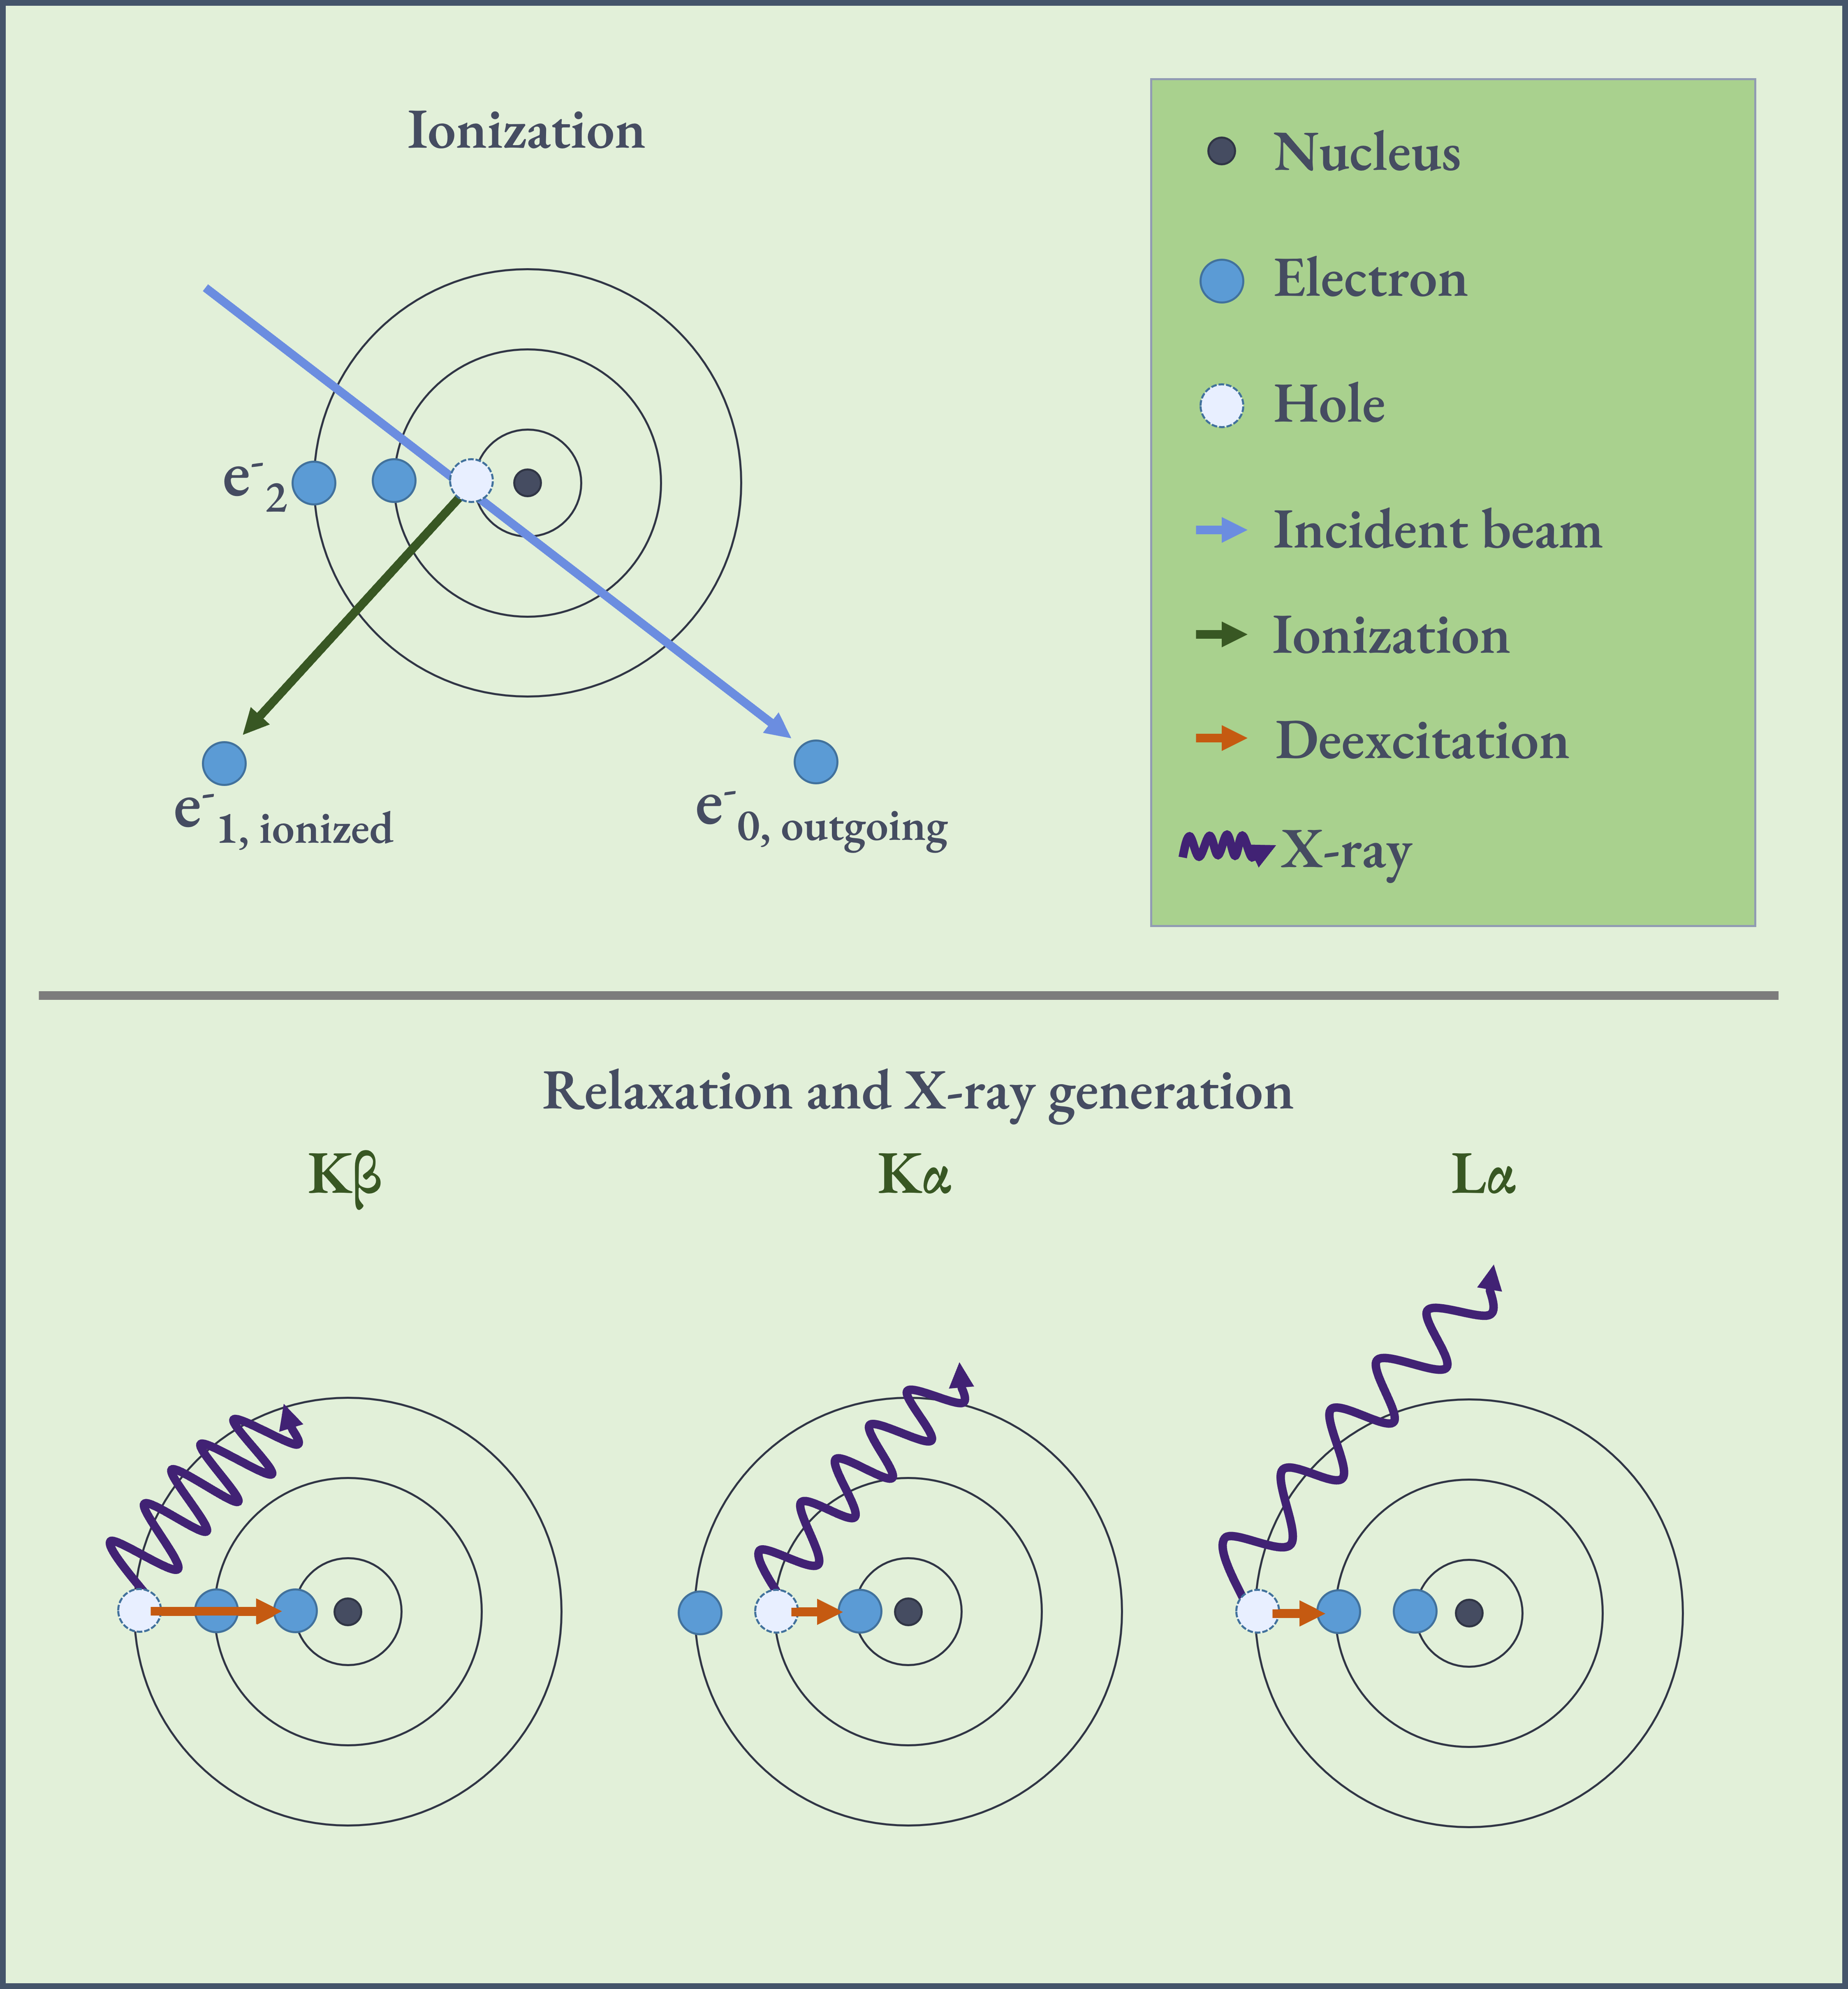
\includegraphics[width=0.7\linewidth]{figures/characteristic_xray_formation.png}
    \caption{
        The formation of characteristic X-rays with the atom as in the Bohr model, where ionization and relaxation is divided into two steps.
        The three relaxations shown produce three characteristic X-rays with different energies.
        Increased energy is illustrated as X-rays with shorter wavelengths.
        % TODO: kommentar fra Ton: Maybe have rings not evenly spaced and use (a) and (b) for panels.
        % jeg tenker nej til kommentaren.
    }
    \label{fig:characteristic_xray_formation}
\end{figure}


The incident electron, marked with the blue arrow and annotated as $\textnormal{e}^-_{0}$, interacts with the atom A and ionizes an inner shell electron, marked with the green arrow and annotated as $\textnormal{e}^-_{1}$.
The ionization leaves a hole in the core orbital.
The electron from the beam have a kinetic energy of E$_{0}$, and loose energy to both breaking the binding energy of the core orbital and to the kinetic energy of the ionized electron.
The binding energy of the core orbital is $E_C$, \textbf{the critical ionization energy}.
$E_C$ is dependent on the atomic number of the atom, as higher Z binds the core electron tighter to the nucleus.
For an ionization to happen, $E_0$ must be higher than $E_C$.
The ionization is given in \cref{eq:theory:xray_formation:characteristic:step1}, and the energy balance is given in \cref{eq:theory:xray_formation:characteristic:step1:energy_balance}.
An X-ray photon with energy higher than the binding energy of the core orbital can also do the ionization.
If a characteristic X-ray photon is doing the ionization, the process is named the fluorescence effect and the resulting photon is called a secondary X-ray.
% The fluorescence effect is covered in \brynjar{cref to section}.

% step 1, ionize the atom
\begin{equation}
    \label{eq:theory:xray_formation:characteristic:step1}
    \textnormal{e}^-_{0 \textnormal{, incident}} + A \rightarrow \textnormal{e}^-_{0 \textnormal{, outgoing}} + A^+ + \textnormal{e}^-_{1 \textnormal{, ionized}}
\end{equation}

% step 1, energy balance
\begin{equation}
    \label{eq:theory:xray_formation:characteristic:step1:energy_balance}
    E_{0 {\textnormal{, incident}}} = E_{0 {\textnormal{, outgoing}}} + E_{C} + E_{1 {\textnormal{, kinetic}}}
\end{equation}




% relax the electron
The second step is the relaxation, illustrated in the bottom part of \cref{fig:characteristic_xray_formation} and expressed in \cref{eq:theory:xray_formation:characteristic:step2}.
An outer shell electron, annotated as $\textnormal{e}^-_{2}$, relaxes to the hole in the inner shell, and the difference in energy between the orbital is emitted as a photon.
This photon is the characteristic X-ray, and the energy of the photon can be expressed as $h\nu$ \cite[Eq. (8.12)]{hollas_modern_2004}.
The energy of the characteristic X-ray is the difference in energy between the ionized orbital and the orbital filling the hole, shown in \cref{eq:theory:xray_formation:characteristic:step2:energy}.
The energy of the characteristic X-ray is usually measured directly in keV \cite[Eq. (4.2b)]{goldstein_scanning_2018}.


% outer orbital relaxation
\begin{equation}
    \label{eq:theory:xray_formation:characteristic:step2}
    \textnormal{e}^-_{2 {\textnormal{, outer shell}}} + \textnormal{"inner shell hole"} \rightarrow \textnormal{e}^-_{2 {\textnormal{, inner shell}}} + h\nu_{\textnormal{X-ray}}
\end{equation}


% the energy of the relaxation
\begin{equation}
    \label{eq:theory:xray_formation:characteristic:step2:energy}
    h\nu_{\textnormal{X-ray}} = E_C - E_{2 {\textnormal{, binding of outer shell}}}
\end{equation}


% comment on the E_C, which is slightly higher than the energy of the photon
% and mass absorption coefficients
As seen in \cref{eq:theory:xray_formation:characteristic:step2:energy}, the critical ionization energy $E_C$ is slightly higher than the energy of the characteristic X-ray ($h\nu_{\textnormal{X-ray}}$).
%energy of the characteristic X-ray is somewhat lower than the critical ionization energy, $E_C$.
If the incident energy on an atom is excatly the critical ionization energy, the atom might be able to absorb this energy and emit a characteristic X-ray, but the probability of this happening is very low \cite{hollas_modern_2004,goldstein_scanning_2018}.
When the incident energy is slightly higher than the energy of the X-ray line, the probability of absorption increase abruptly.
The abrupt increase of the absorption slightly above an characteristic X-ray line is called an \textbf{absorption edge} \cite{goldstein_scanning_2018}.
The probability of absorption is given by the \textbf{mass absorption coefficient}, noted as $\mu_\rho$ in this work, which is dependent on the energy of the X-ray.
$\mu_\rho$ for a material can be plotted as a function of the energy of the X-ray, and the absorption edges are clearly visible as nearly vertical lines in the plot.
\cref{fig:mass_absorption_coefficients} shows $\mu_\rho$ for GaAs in panel (a) and GaSb in panel (b), with characteristic X-ray energies marked with vertical lines.
The mass absorption coefficient, or mass attenuation coefficient, is defined as the materials attenuation coefficient normalized by the density of the material \cite{goldstein_scanning_2018}.
The normalization by the density makes the mass absorption coefficient a material property which tells how likely a mass of the material is to absorb X-rays.
It is common to write the mass absorption coefficient as $\mu/\rho$, but it is written $\mu_\rho$ in this work to clearly show that it is referring to one specific value for the material, which have the unit cm$^2$/g.
% The energy required to ionize an electron, $E_C$, can be referred to as the \textbf{absorption edge}, because the absorption an atom does increase abruptly at the energy of the absorption edge.
The mass absorption coefficient of a mixture of elements, e.g. GaAs, is a combination of the mass absorption coefficients of the elements in the mixture, and can be calculated with HyperSpy\footnote{\url{http://hyperspy.org/hyperspy-doc/current/api/hyperspy.misc.material.html}}.
HyperSpy contains the mass absorption coefficients of the elements as a function of energy, with data from a NIST database \cite{nist_xraydatabase_hyperspy}.
\cref{fig:background_absorptionEdgeSi} combines an EDS spectrum with the mass absorption coefficient of Si, and shows how the absorption increases at the absorption edge.
As $\mu_\rho$ is relatively low at the energy of the characteristic X-ray, the probability of absorption is low.
For example, a Fe K$\alpha$ X-ray in Fe has a low probability of ionizing the same transition in another Fe atom.
This makes an element more transparent to its own characteristic X-rays \cite[Ch. 4.4]{goldstein_scanning_2018}.
% In other words, because of the absorption edges an element is more transparent to its own characteristic X-rays \cite[Ch. 4.4]{goldstein_scanning_2018}.
After the sharp increase at the absorption edge, the probability of absorption decreases.
This makes the probability of ionization greatest when the energy is just above the critical ionization energy.
If the energy is significantly higher than the critical ionization energy, the probability of ionization is lowered \cite[p. 78]{curry_radiology_k_absorption}, because $\mu_\rho$ continues to decrease.
This implies that using a higher energy for ionization is not necessarily better, which is discussed more in \cref{theory:eds:user_controlled_parameters}.


When the outer shell electron is relaxed, a new hole is generated in the outer shell.
This leads to a cascade of relaxation events, but the energies of these transitions are too low to emit characteristic X-rays.
These and other non-radiative relaxations will not be discussed further.


% figures/mass_absorption_coefficients.pdf
\begin{figure}[phtb]
    \centering
    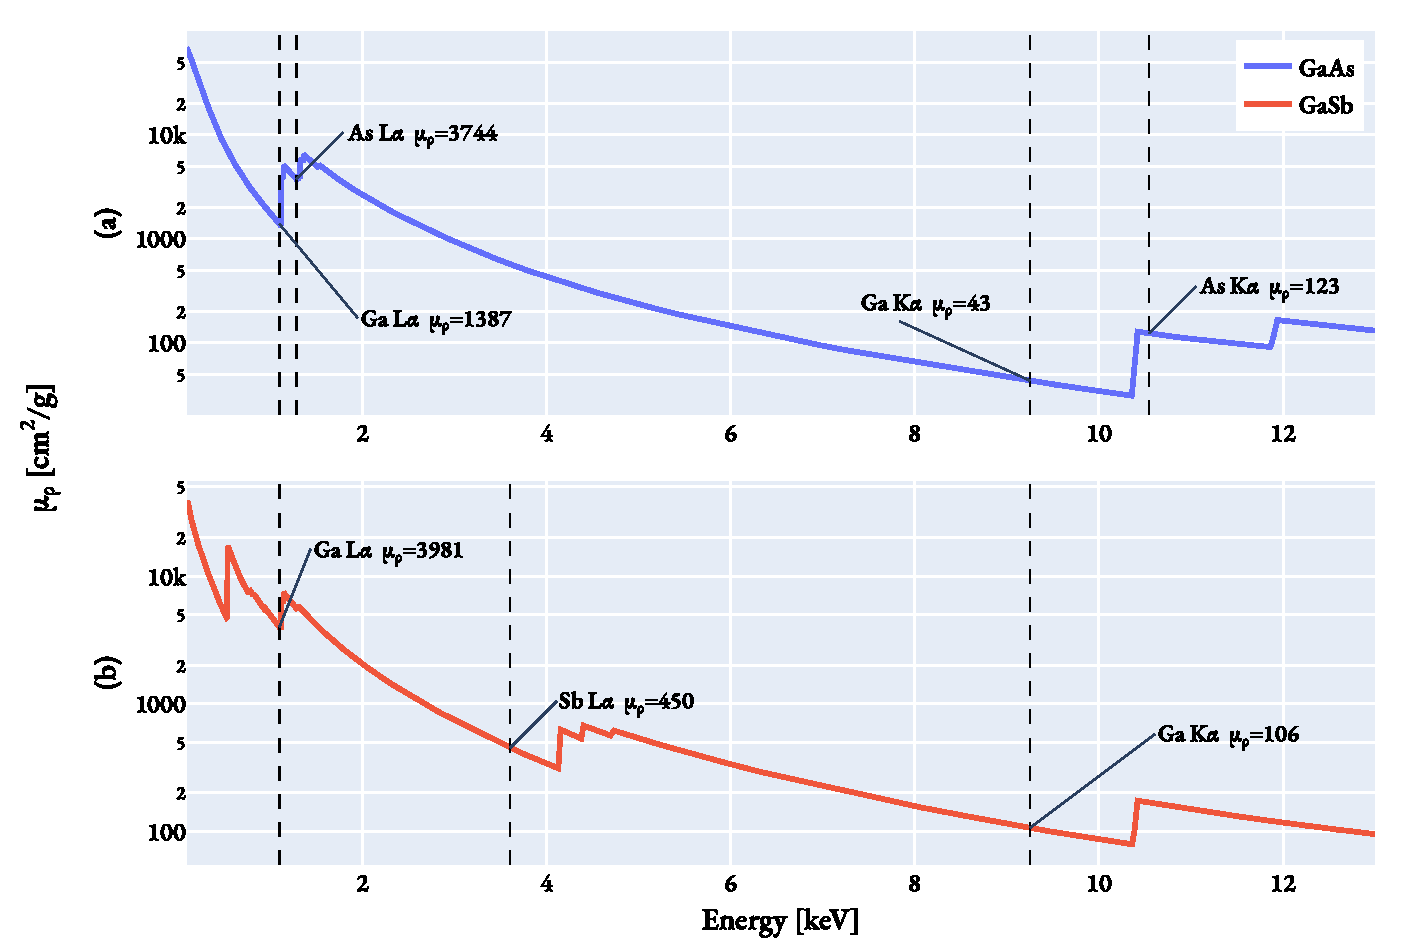
\includegraphics[width=0.95\textwidth]{figures/mass_absorption_coefficients.pdf}
    \caption{
        The mass absorption coefficients ($\mu_\rho$) of (a) GaAs and (b) GaSb, with characteristic X-ray energies marked with vertical lines.
        Note how much $\mu_\rho$ increases at the absorption edge, which is slightly higher than the energy of the characteristic X-ray.
        The absorption edge in GaSb around 0.5 keV is the M-lines of Sb, and the additional steps after Sb L$\alpha$ is the L$\beta$ lines.
        Annotated numbers are for $\mu_\rho$ in units of cm$^2$/g.
    }
    \label{fig:mass_absorption_coefficients}
\end{figure}


% mention Auger electrons, because of the fluorescence (quantum) yield
% the kinetic energy is essential for Auger electrons, i.e. E_{2_{\textnormal{kinetic}}}
In the second step of the X-ray formation process described in \cref{eq:theory:xray_formation:characteristic:step2}, there is also a probability that the energy from the relaxation is not used to emit a photon, but used to eject another electron from a higher energy orbital, giving it kinetic energy.
This results in the ejection of two electrons, one from the core orbital and another from the higher energy orbital, known as an Auger electron.
Auger electrons are useful for surface studies since they can penetrate approximately 2 nm of solid material, thereby not escaping from inside the sample.
The emitted X-rays, on the other hand, are isotropically emitted from a large volume and can penetrate up to 4000 nm, as the absorption of X-ray photon is far less likely than that of a charged electron. %, making them the signal in EDS. 
The ratio of characteristic X-ray photons to Auger electrons is known as the \textbf{fluorescence (quantum) yield}, $\omega$.

% fluorescence yield, definition
\begin{equation}
    \label{eq:theory:theoreticalxray:yield}
    \omega = \frac{\textnormal{X-ray photons}}{\textnormal{Auger electrons}}
\end{equation}

The fluorescence yield is heavily dependent on the ionized atom, with in general higher fluorescence yields for heavier atoms.
$\omega$ is also dependent on the shell that is ionized, with the typical trend being $\omega_K$ > $\omega_L$ > > $\omega_M$ \cite[p. 267]{goldstein_scanning_2018}.
The dependence on Z and the shell is shown in \cref{fig:theory:fluorescence_yield}, a figure adapted from Goldstein \cite[Fig. 4.3 (d)]{goldstein_scanning_2018}.

% figure/fluorescence_yield_Goldstein_Fig4.3.d.png
\begin{figure}[ht]
    \centering
    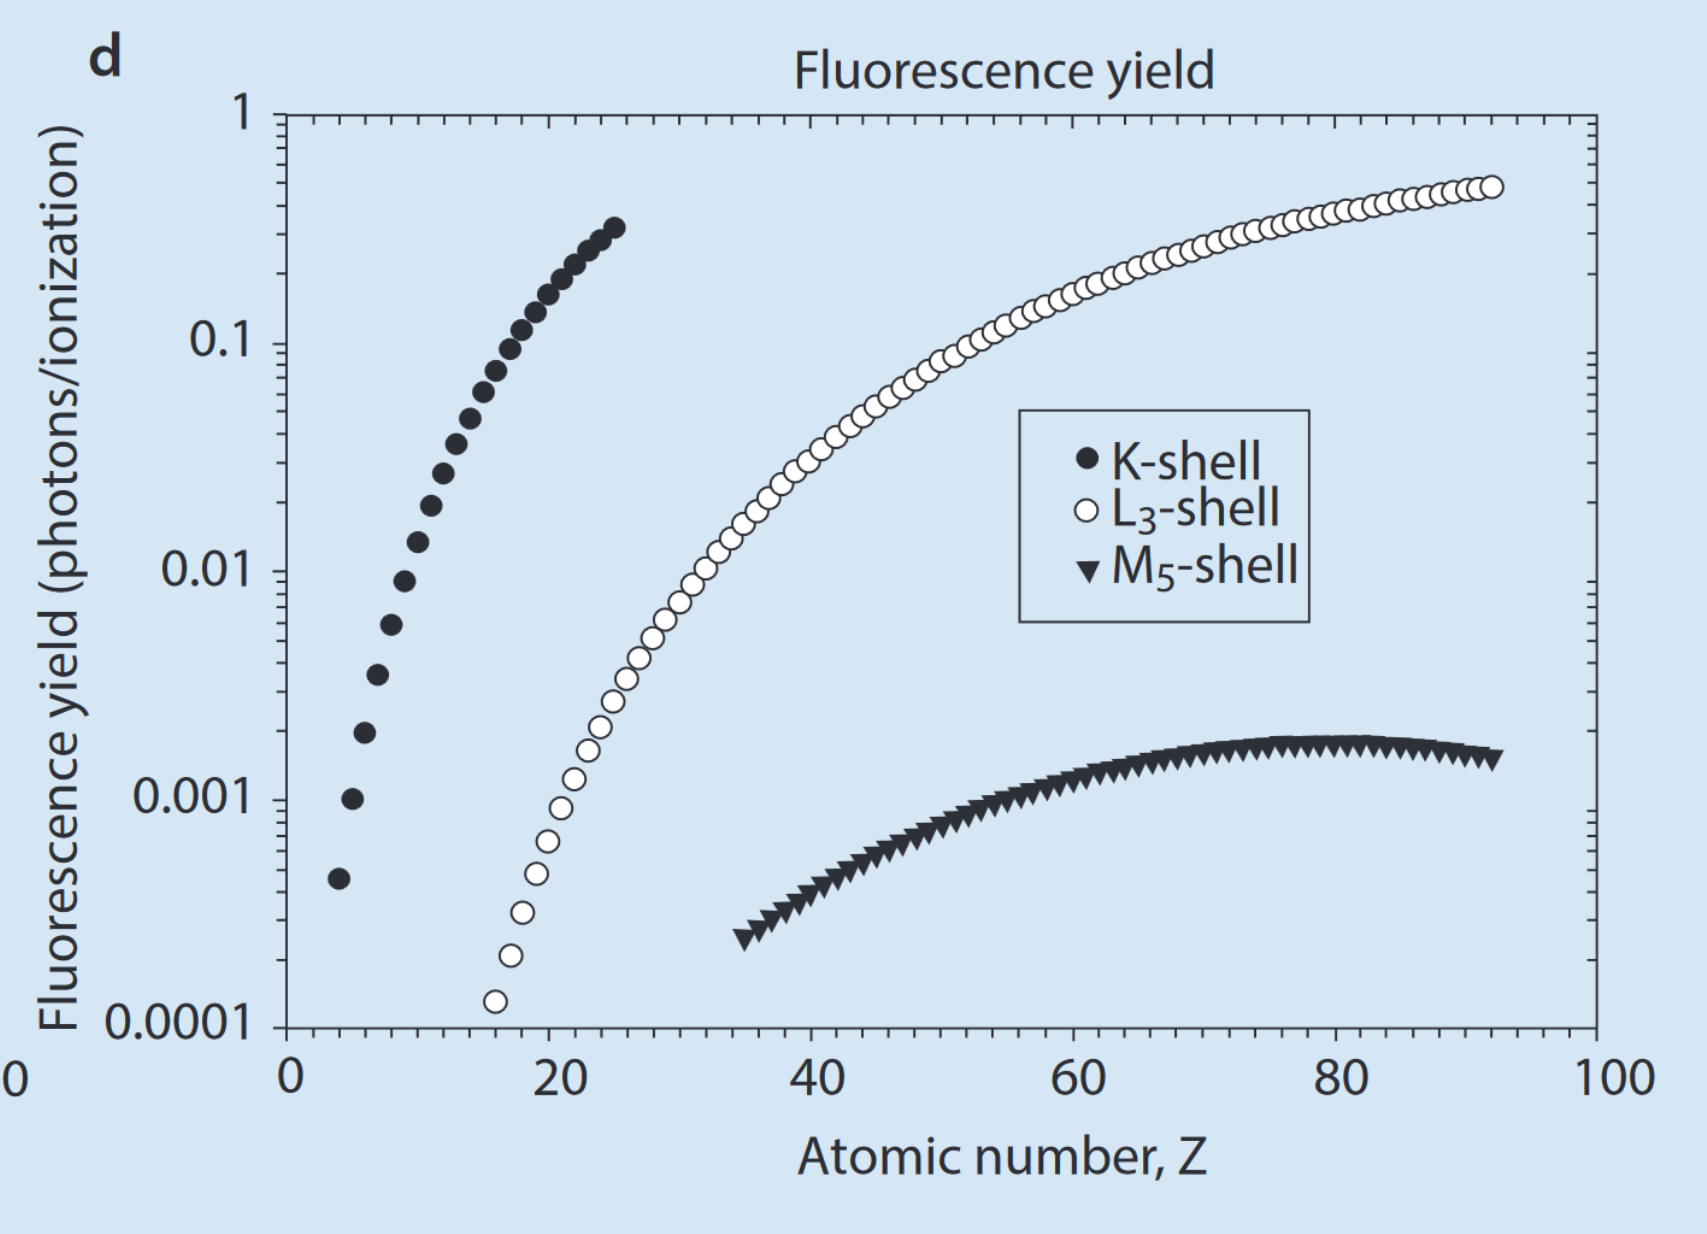
\includegraphics[width=0.7\textwidth]{figures/fluorescence_yield_Goldstein_Fig4-3-d.png}
    \caption{
        $\omega$ for K-, L- and M-shell, as a function of atomic number Z.
        Adapted from \cite[Fig. 4.3 (d)]{goldstein_scanning_2018}.
    }
    \label{fig:theory:fluorescence_yield}
\end{figure}








\subsection{The naming convention of characteristic X-rays}
\label{theory:xray_formation:naming}

% add motivation for why this is included.

% The next two paragraphs explaining the naming convention is not essential for the understanding of the thesis, but is included for completeness and was made out of curiosity.
% % The reader can skip this section knowing that it is the Siegbahn notation which is used in this thesis.
% The author was curious about the origin of the naming convention, as it is a system that follows some logical rules, while also being somewhat cryptic.
% Looking at possible orbital transitions in a schematic figure like \cref{fig:theory:xray_formation:lines}, the first letter makes sense, but the Greek letter and the number seems to be less systematic.

This subsection explains the Siegbahn naming convention for characteristic X-rays, which is used in this thesis.
The Siegbahn notation is based on the Bohr model of the atom and intensities of the X-ray lines in a spectrum.
As the Bohr model is a simplification of the actual atom, the Siegbahn notation is somewhat confusing when looking at the actual orbital transitions, as they are illustrated in \cref{fig:theory:xray_formation:lines}.
It should be noted that The International Union of Pure and Applied Chemistry (IUPAC) made a new and systematic naming convention for X-ray lines \cite{IUPAC_nomenclature1991}.
However, the Siegbahn notation is still the most used convention \cite[Ch. 4.2.4]{goldstein_scanning_2018}, for example used in HyperSpy, and is therefore used in this thesis.
Additionally, the IUPAC notation is not connected to the intensity of the X-ray lines, which is a useful property when discussing the X-ray lines in a spectrum.
A table showing the correspondence between the two naming conventions is shown in \cref{tab:theory:naming_convention}.
The IUPAC naming convention notes both the orbital in the inner and outer shell, thus \cref{tab:theory:naming_convention} shows what the possible observable transitions in EDS between 0.1 and 25 keV are.
\cref{fig:theory:xray_formation:Sb_L-peaks} shows the actual L-lines from Sb in an EDS spectrum.



% figure with the naming convention
\begin{figure}[p]
    \centering
    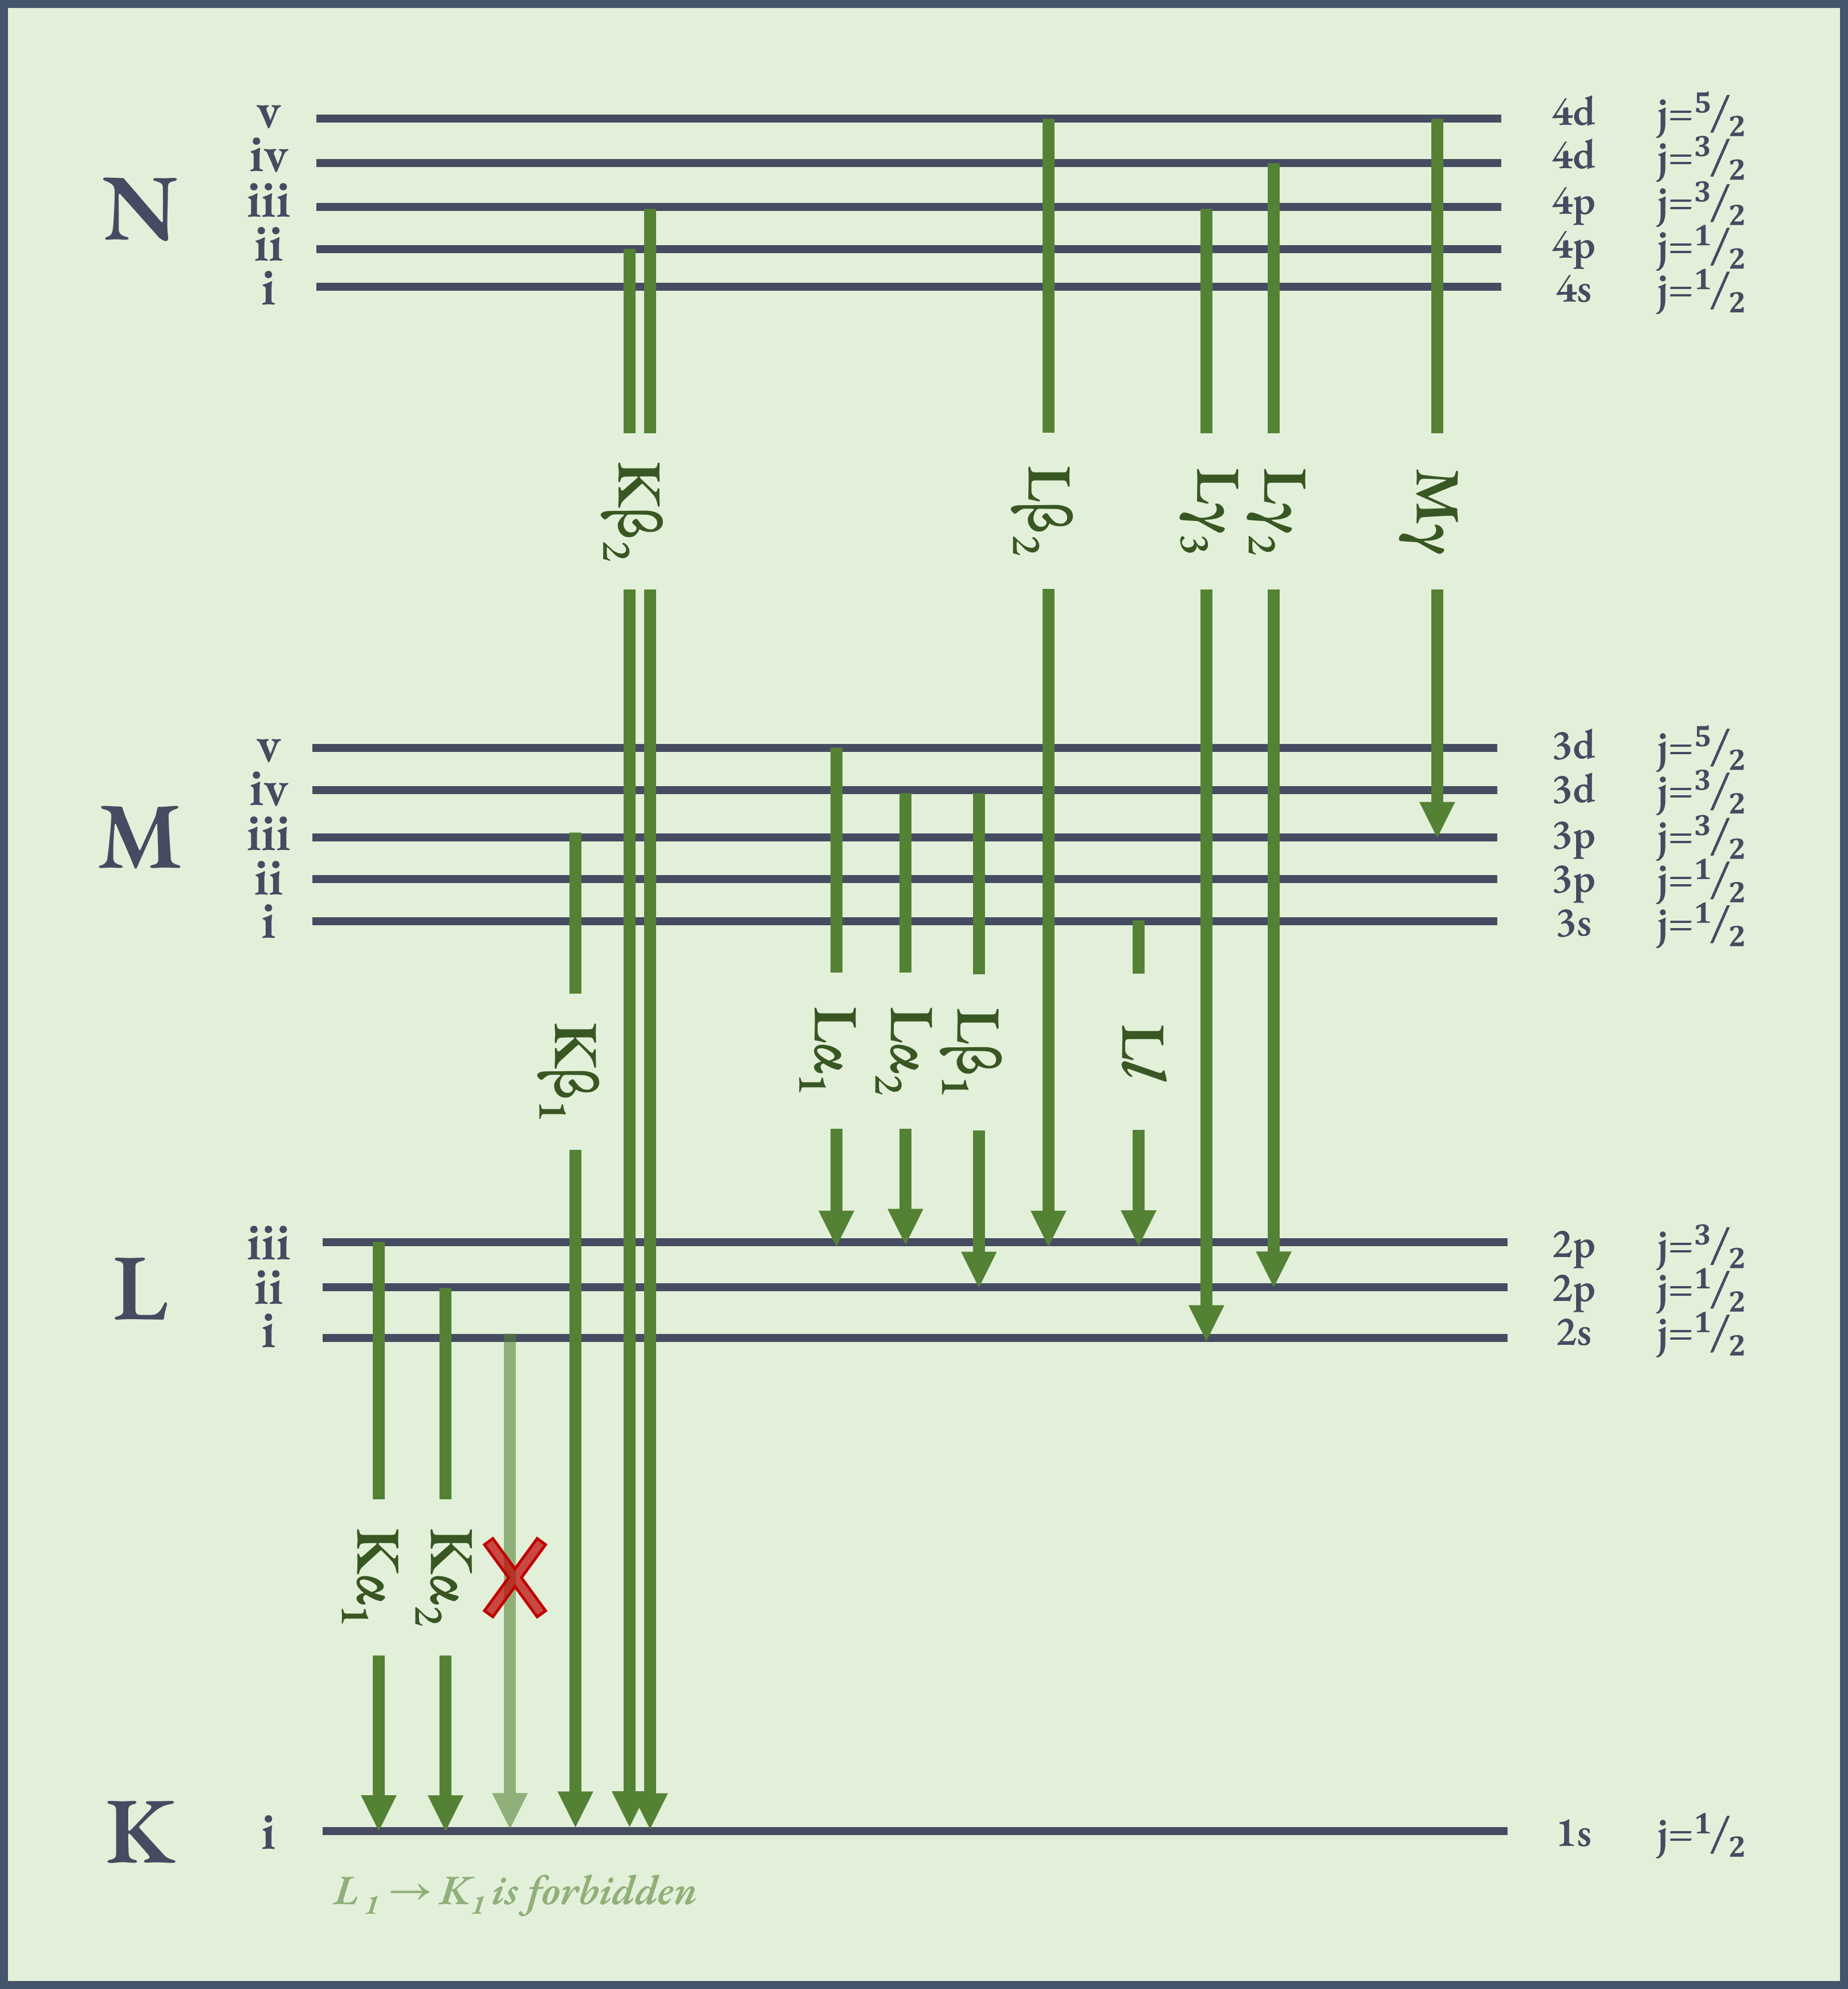
\includegraphics[width=0.95\linewidth]{figures/transition_lines.png}
    \caption{
        Schematic of the electron relaxations with their naming convention.
        The horizontal lines are the orbitals in the different shells, and the arrows are the relaxations.
        Higher orbitals have higher energy, but the distance between the orbitals is not to scale.
        The shell name and orbital number are shown on the left, and quantum number $n$, $l$, and $j$ are shown on the right.
        The azimuthal quantum number $l$ is included as the orbital names, i.e. $s$, $p$, and $d$.
        The figure also show one forbidden line, where neither $l$ nor $j$ change.
        \cref{tab:theory:naming_convention} include more transitions.
        \cref{fig:theory:xray_formation:Sb_L-peaks} shows the Sb L-lines in a spectrum.
    }
    \label{fig:theory:xray_formation:lines}
\end{figure}


% table with naming convention
\begin{table}[p]
    \centering
    \caption{
        The naming of characteristic X-ray lines.
        The table includes lines observed in EDS from $0.1$ to $25$ keV.
        The IUPAC notation is first the inner orbital, then the outer orbital.
        The Siegbahn notation is the inner shell and the lines relative intensity.
        \cref{fig:theory:xray_formation:lines} visualize some lines in the table.
        As seen for the M transitions, the Siegbahn notation does not cover all possibilities.
        Remake of Table 4.1 in Goldstein \cite{goldstein_scanning_2018}.
    }
    \label{tab:theory:naming_convention}
    \begin{tabular}{cl|cl|cl}
        \hline
        \textbf{Siegbahn} & \textbf{IUPAC} & \textbf{Siegbahn} & \textbf{IUPAC} & \textbf{Siegbahn} & \textbf{IUPAC}      \\
        \hline
        K$\alpha$$_1$     & K-L$_3$        & L$\alpha$$_1$     & L$_3$-M$_5$    & M$\alpha$$_1$     & M$_5$-N$_7$         \\
        K$\alpha$$_2$     & K-L$_2$        & L$\alpha$$_2$     & L$_3$-M$_4$    & M$\alpha$$_2$     & M$_5$-N$_6$         \\
        K$\beta$$_1$      & K-M$_3$        & L$\beta$$_1$      & L$_2$-M$_4$    & M$\beta$          & M$_4$-N$_6$         \\
        K$\beta$$_2$      & K-N$_{2,3}$    & L$\beta$$_2$      & L$_3$-N$_5$    & M$\gamma$         & M$_3$-N$_5$         \\
                          &                & L$\beta$$_3$      & L$_1$-M$_3$    & M$\zeta$          & M$_{4,5}$-N$_{2,3}$ \\
                          &                & L$\beta$$_4$      & L$_1$-M$_2$    &                   & M$_3$-N$_1$         \\
                          &                & L$\gamma$$_1$     & L$_2$-N$_4$    &                   & M$_2$-N$_1$         \\
                          &                & L$\gamma$$_2$     & L$_1$-N$_2$    &                   & M$_3$-N$_{4,5}$     \\
                          &                & L$\gamma$$_3$     & L$_1$-N$_3$    &                   & M$_3$-O$_1$         \\
                          &                & L$\gamma$$_4$     & L$_1$-O$_4$    &                   & M$_3$-O$_{4,5}$     \\
                          &                & L$\eta$           & L$_2$-M$_1$    &                   & M$_2$-N$_4$         \\
                          &                & L$l$              & L$_3$-M$_1$    &                   &                     \\
        \hline
    \end{tabular}
\end{table}

% figure with actual L-peaks in Sb
\begin{figure}[p]
    \centering
    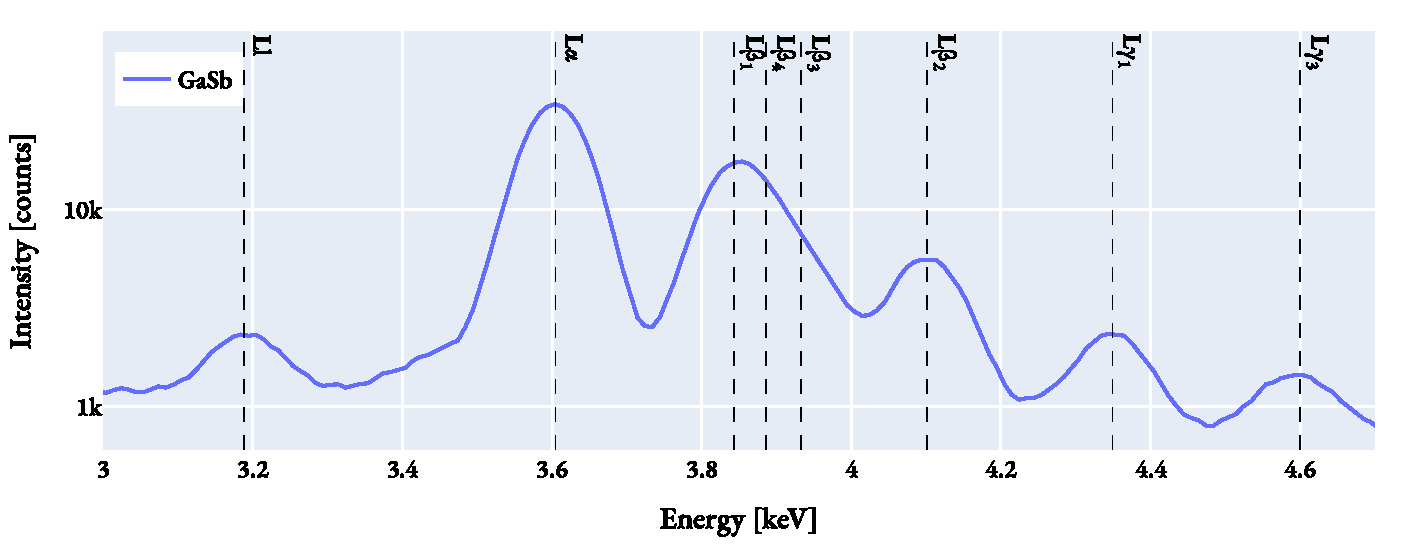
\includegraphics[width=0.99\linewidth]{figures/Sb_L-peaks_30kV_50pA.pdf}
    \caption{
        Example spectrum of the Sb L-peaks in a GaSb wafer.
        Taken at 30 kV, 50 pA, process time 6, live time 120 s, ICR at 17000 cps, and 43\% DT.
        For further experimental details, see \cref{ch:method}.
    }
    \label{fig:theory:xray_formation:Sb_L-peaks}
\end{figure}



% Old stuff, refined

% The Siegbahn notation
The transition lines are grouped and named based on the orbital the vacancy is in, and the orbital the electron is relaxed from.
The naming convention is semi-systematic because it is the original empirical system published in Nature by the Swedish physicist Kai Siegbahn in 1916 \cite{siegbahn_relations_1916}, without the modern theoretical knowledge on orbitals.
% K, L, M
The X-rays lines categorized in families which are named by the shell in the Bohr model where the vacancy is, i.e. the principal quantum number $n$ of the vacancy orbital.
Relaxations to the innermost shell $n=1$ is named K-transitions, relaxations to $n=2$ is L-transitions, relaxations to $n=3$ is M-transitions.
% LOL, Github Copilot foreslo setningen under utfra "K, "
% K, L, and M are the first letters in the German words for the shells, Korbital, Lorbital, and Morbital.
% alpha, beta, gamma
The lines in the families are further grouped with Greek letters or other symbols, where the order is related to their relative intensity: $\alpha > \beta > \gamma > \nu > \zeta$.
Additionally, the minor L-shell transitions in split into families notated with Latin letter subscripts: l, s, t, u, and v \cite[Ch. 4.2.4]{goldstein_scanning_2018}.
% subscripts
Lines which are closely related are given a subscript number, where 1 is the most intense line.
As the energy resolution of EDS is limited, a single peak in a spectrum can consist of multiple transitions which are closely related, e.g. K$\alpha_1$ and K$\alpha_2$ making the K$\alpha$ line.
Resolving K$\alpha_1$ and K$\alpha_2$ in EDS is usually first possible for elements heavier than tin with $ Z = 50$ \cite[Ch. 8.2.2.3]{hollas_modern_2004}. %, where the $\Delta E = 227.3$ eV.
Heavier element have both more possible lines and more resolved lines, as the orbitals have higher energy differences.
\brynjar{Legge til kommentar om intensity, som er inkludert i Siegbahn med ikke i international. Som gir Siegbahn en praktisk fordel.}
% dropping the stuff about spin-orbit coulpling


% total naming with example
Putting these three naming conventions together, we name the transition $\textnormal{L}_3 \rightarrow \textnormal{K}_1$ as K$\alpha_1$, and $\textnormal{L}_2 \rightarrow \textnormal{K}_1$ as K$\alpha_2$, with more examples in \cref{fig:theory:xray_formation:lines}.
The transition $\textnormal{L}_1 \rightarrow \textnormal{K}_1$ has $\Delta l =  0$ and is thus forbidden by the selection rules, see \cref{eq:theory:selectionrules}.
In gallium the K$\alpha_1 = 9252$ eV and K$\alpha_2 = 9223$ eV \cite{thompson_x-ray_2004} have an energy difference of $\Delta E = 27$ eV, which is too low to be resolved in EDS.
% \ton{I had a figure with the Ga Ka peak in the project thesis. Should I include it?}
% # now i have Sb 



% \clearpage

\subsection{Energy and width of characteristic X-rays}
\label{theory:xray_formation:energy}

% what the energy is

The energy of the X-rays is the energy difference between the orbitals, and the spread in energy from a single line is typically between 1-10 eV.
The energy difference between the orbitals increase with atomic number Z, as the electrons are bound tighter to the nucleus.
A table with the energies of the relevant characteristic X-rays in this thesis is given in \cref{tab:theory:lineEnergies}.
The table also includes the relative weight of the lines, which is the intensity of the line relative to the strongest line in the lines group.
The most central parts of the energy of the X-rays have been mentioned earlier, but the width of the lines is also important.
This section also includes where the energy of X-rays can be found.


% widths
The natural width of Mn K$\alpha$ is around 1.5 eV, while the measured width in EDS is typically between 120-140 eV \cite[Ch. 16.1.1]{goldstein_scanning_2018}.
This peak broadening is due to counting statistics and instrument electronics, which is discussed in \cref{theory:eds:hardware}.
The broadness of the peaks in EDS increase with energy, and the peak broadening effect is the most limiting factor for the energy resolution of EDS.
The change from lines to broadened peaks is illustrated in \cref{fig:eds_theoretical2realSpectrum}.
Data tools have been developed for EDS to identify and separate peaks which overlap in energy, like peak deconvolution and peak fitting.
% From Ton, rewrite: To achieve higher energy resolution, the wavelength rather than energy can be analyzed. This so called wave length dispersive (WDS) has energy resolution of ca. 10 eV [Goldstein, Williams and Carter], but is less practical easy than EDS and will not be discussed further here.
Higher resolution can be achieved by analyzing the wavelength rather than the energy of the X-rays.
This is called wavelength dispersive X-ray spectroscopy (WDS), and has an energy resolution of ca. 10 eV \cite{goldstein_scanning_2018}, but is less practical than EDS and will not be discussed further here.


% where to find the energy
% issues when a line is not listed in your source
The energy of characteristic X-rays has been measured and calculated, and published in tables and databases.
One source is the X-ray Data Booklet \cite{thompson_x-ray_2004}, another is one of the NIST X-ray databases, like the "X-Ray Transition Energies Database" \cite{nist_xraydatabase}.
The Python package HyperSpy includes an elemental database with the energy of characteristic X-rays \cite{hyperspy_1.7.1}, which is based on NIST database 66, "X-Ray Form Factor, Attenuation, and Scattering Tables" \cite{nist_xraydatabase_hyperspy}.
The different sources are focused on certain areas, like how the NIST database 128 includes experimental data, while the HyperSpy database is less comprehensive but faster to use.
An analyst should be aware of the limitations of the used source, like how the HyperSpy database does not include the M-lines for Sb.
% Trusting a source blindly can lead 
The limited energy resolution of EDS combined with overlapping peaks can lead to mislabeling in the qualitative analysis, which is discussed in \brynjar{Ref to discussion on this}.
The reason for the missing M-lines in the HyperSpy database is probably a down prioritization due to the low intensity of these M-lines, which is discussed in the next section.



\subsection{Intensity of characteristic X-rays}
\label{theory:xray_formation:intensity}

\brynjar{Lese over denne delen, flyttet litt rundt på greier.}

% some transitions are present, but intensity differs
% the selection rules, forbidden transitions
Just as the energy of the X-ray lines increase with atomic number, the number of possible lines increase too.
As the energy difference between orbitals increase, close lines like K$\alpha_1$ and K$\alpha_2$ are, as explained earlier, resolved.
The number of possible lines increase with Z because there are more orbitals giving more possible transitions.
However, not all transitions are allowed, and their intensity varies.
The selection rules, given in \cref{eq:theory:selectionrules}, govern which transitions are allowed.
The selection rule applies to the electron which is being relaxed, and it is \cite[Sec. 8.2.2.2]{hollas_modern_2004}:

\begin{equation}
    \label{eq:theory:selectionrules}
    \Delta n \ge 1;\qquad \Delta l  = \pm 1;\qquad \Delta j = 0, \pm 1
\end{equation}

where $\Delta n$ is the change in principal quantum number, $\Delta l$ is the change in orbital angular momentum, and $\Delta j$ is the change in total angular momentum.
The orbital angular momentum is also called the azimuthal quantum number.
The three quantum numbers are included in \cref{fig:theory:xray_formation:lines}, for K to N$_5$.
Lines which are forbidden by the selection rules, like the transition from K to L$_1$, have an intensity of zero.
Some lines are allowed, but have too low intensity to be detected in EDS.


% moved, ionization cross-section
The ionization cross-section is the probability of an ionization for a given line, originally described by Bethe \cite{inokuti_on_bethe_1971} as:
\begin{equation}
    \label{eq:ionizationcrosssection}
    \sigma_T = \frac{\pi e^4 b_s n_s}{E_0 E_C}  \log\left(\frac{c_s E_0}{E_C}\right)
\end{equation}

where $\sigma_T$ is the total scattering cross-section, $e$ is the elementary charge, $n_s$ is the number of electrons in the ionized shell, $b_s$ and $c_s$ are constants for the shell of ionization, $E_0$ is the incident electron energy, and $E_C$ is the critical ionization energy.
The ionization cross-section is strongly dependent on the atomic number of the element of interest, and higher Z have higher $E_C$.


% the intensity of allowed lines
The generated intensity of the allowed lines is proportional to the electron dose from the probe, the number of atoms and the atomic weight of the given element, the fluorescence yield, and the ionization cross-section. %the detector efficiency, and the size of the detector.
The electron dose is a function of the probe current and the acquisition time.
The dependency of the number of atoms of the given element is crucial, as this is the basis for the quantitative analysis in EDS.
The factors mentioned above are discussed further in the section on quantitative analysis in EDS \cref{theory:quantitative}.
Calculating the intensity of characteristic X-ray lines from bulk specimen is not trivial, but in Goldstein there is an experimentally based equation for this: \cite[Eq. 4.8]{goldstein_scanning_2018}:
% Goldstein includes an experimentally based equation for the intensity of X-rays from bulk specimen \cite[Eq. 4.8]{goldstein_scanning_2018}:

\begin{equation}
    \label{eq:theory:xray_formation:intensity}
    I \approx i_p (U-1)^n
\end{equation}

where $I$ is the relative intensity of X-rays from different atomic numbers and shells, $i_p$ is the probe current, $U$ is the overvoltage (covered in \cref{theory:eds:user_controlled_parameters}), and $n$ is a constant which depends on Z and the excited orbital.
It is stated in Goldstein that $n$ is typically between 1.5 and 2.0, and the equation is based on the work presented and published by Lifshin et al. 1980 \cite{lifshin1980}.



% intensity of formation is not the same as intensity of detection
Additionally, the intensity of detected X-rays is not the same as the intensity of the X-rays which are generated.
The probability of absorption is a function of density and increase with the travel distance.
Photons with lower energy are absorbed more easily than photons with higher energy, i.e. the escape depth of the X-rays increase in general with energy.
Expressed in terms of the absorption coefficient $\mu$ and the path length $l$, the intensity is reduced by:

\begin{equation}
    \label{eq:theory:xray_formation:escape}
    I_{\textnormal{escaped}} = I_{\textnormal{generated}} \exp(-\mu l)
\end{equation}

where $\mu$ is dependent on the material (Z) and the energy of the X-rays.
When a thin specimen (<30 nm) is analyzed \cite{watanabe_williams_zeta_2006}, the absorption effect can be ignored, the so-called thin film approximation used in Cliff-Lorimer quantification, see \cref{theory:quantitative}.
When thicker samples are analyzed, the absorption and fluorescence effect must be taken into account for the quantitative analysis \cite{goldstein_scanning_2018}.
Escape probability and depth is also dependent on the absorption edges present.
When an X-ray photon is absorbed within the specimen, it can ionize an atom and generate a new X-ray with a lower energy, which is the previously mentioned fluorescence effect.
When thin samples are analyzed, the fluorescence effect can be ignored, but when thicker samples are analyzed, the fluorescence effect can be significant.
For secondary fluorescence to happen, a characteristic X-ray must be absorbed, and it must have higher energy than the critical ionization energy of other lines in the material.
If the absorbed X-ray have an energy higher than the $E_C$ + 5 keV of the other lines, the fluorescence effect is negligible \cite[p. 306]{goldstein_scanning_2018}.
The fluorescence effect is also dependent on the path length of the X-rays in the specimen.
Compensation for the fluorescence effect is discussed in \cref{theory:quantitative:principle}.









\subsection{Background X-rays}
\label{theory:xray_formation:background}

% further down
% Lastly, the \textbf{background X-rays} are formed by the deacceleration of the incident beam electrons because of the Coulomb fields of the atoms in the specimen, and this deacceleration of charged particles emits photons \cite{notaros_electromagnetics_2010}.
% The background X-rays are white noise, giving no information about the sample, and is generated in the whole interaction volume.

% intro
The detected spectrum contains more than peaks from characteristic X-ray lines as discussed so far.
In addition to the characteristic X-rays generated, the electron beam generates background X-rays.
The background radiation is also called the bremsstrahlung, breaking radiation, and the continuum radiation.
These X-rays are formed by the deacceleration of the incident beam electrons in the Coulomb fields of the atoms in the specimen, where the electron loose kinetic energy.
This effect includes both velocity and directional changes, and the changes in the incident electrons paths are visualized in a Monte Carlo simulation in \cref{fig:montecarlo_BSE}.
Acceleration and deacceleration of charged particles emits photons \cite{notaros_electromagnetics_2010}.
The background X-rays are white noise, giving no information about the sample.
However, the background radiation can be used to calculate at least one parameter describing the detector performance, namely the Duane-Hunt limit covered in \cref{theory:eds_performance:duanehunt}.
Through pre-modelling of the background based on the sample geometry and composition, the background signal can also be used to check for incorrect tilt or shadowing \cite{edax_insight_2019}.
To do accurate qualitative analysis, the background radiation must be subtracted from the total spectrum.
This can be done in multiple ways, like pre-modelling, linear interpolation, background filtering, and background modelling \cite{liao2006practical}
In this thesis, background modelling is used, where the background is modelled as a polynomial function of the energy.
Modelling of the background is discussed in \brynjar{Ref to right section}.


% the energy, 1/E
The energy lost by an electron in a single scattering event can be any value from almost zero to the incident electron energy, $E_0$.
In other words, the background X-rays can have any energy from around 100 eV to the incident electron energy \cite[Ch. 4.3]{goldstein_scanning_2018}.
The probability of a background X-ray with energy E can be described by the Kramer's cross-section and empirically estimated as:

% N(E) = (K Z (E_0-E))/E
\begin{equation}
    \label{eq:theory:xray_formation:background}
    N(E) = \frac{K Z (E_0-E)}{E}
\end{equation}

where $N(E)$ is the number of background X-rays with energy $E$, $K$ is Kramer's constant, $Z$ is the atomic number of the specimen, and $E_0$ is the incident electron energy.
As seen in \cref{eq:theory:xray_formation:background}, the formation of background radiation is inversely proportional to the energy of the X-rays, i.e. $N(E) \propto 1/E$.
However, the low energy X-rays formed inside the specimen are absorbed by the specimen, resulting in a difference between the detected and the generated background X-rays.
The difference between the generated and detected background X-rays is visualized in \cref{fig:background_xrays}.
The detected background X-rays have a peak in the low keV region, depending on the specimen and acceleration voltage.
The peak is typically around 2 keV.
When the energy approach zero, the detected background decrease rapidly.
In addition, the absorption edges of the materials in the specimen influence the intensity of the background radiation, as described in \cref{theory:xray_formation:characteristic}.
As the specimen absorbs more above an absorption edge, the intensity of the background can be observed to decrease abrupt just above a strong absorption edge \cite[p. 59]{goldstein_scanning_2018}.
This effect was observed in the authors project thesis, with a suggestion of splitting the background modelling into two parts, one for the low energy background and one for the high energy background \cite{project_report}.
The effect of the absorption edge was observed to variate, being strongest for the highest peak in the lower keV region.
An example of the effect of the absorption edge is shown in \cref{fig:background_absorptionEdgeSi}.
This correction could be a potential improvement of the model fitting \cite{hyperspy_1.7.1,nilsen_factorless_2021}, and thus making the qualitative analysis more accurate, especially for low keV analysis.


% figures/background_generated_detected.pdf
\begin{figure}[pht]
    \centering
    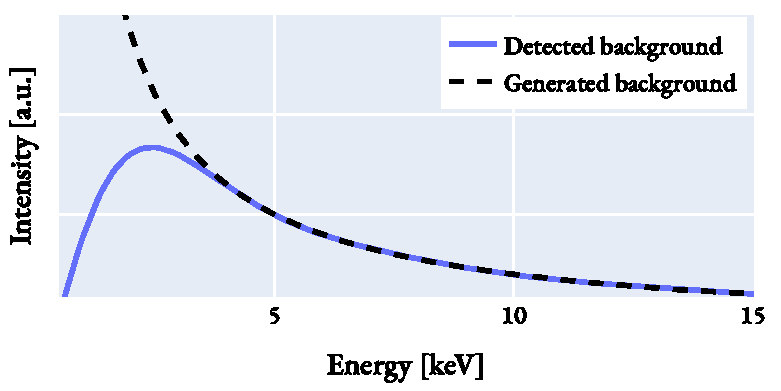
\includegraphics[width=0.8\linewidth]{figures/background_generated_detected.pdf}
    \caption{
        The difference between the generated and detected background X-rays.
        The detected background is shown in blue, and the generated background is shown in the dashed black line.
    }
    \label{fig:background_xrays}
\end{figure}

% figures/background_absorptionEdge_Si.pdf
\begin{figure}[pht]
    \centering
    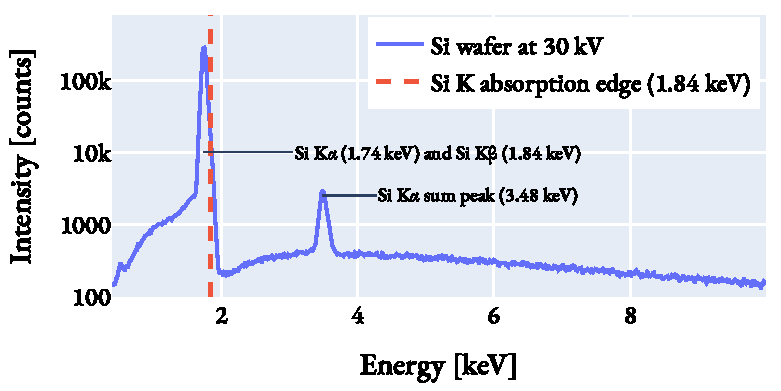
\includegraphics[width=0.95\linewidth]{figures/background_absorptionEdge_Si.pdf}
    \caption{
        The effect of the absorption edge on the background radiation.
        The spectrum in blue is from a Si wafer and the red dashed line is the Si K absorption edge at 1839 eV \cite{absorptionEdges_1967,hyperspy_1.7.1}.
        The background is abruptly reduced just above the absorption edge.
        The green dotted line is the mass absorption coefficient ($\mu_\rho$) of Si as a function of energy, which increase with a factor of 10 at the absorption edge.
        The spectrum shows the overlapping Si K$\alpha$ and K$\beta$ peaks, the Si sum peak and a small O K$\alpha$ signal.
        Sum peaks are discussed in \cref{theory:eds:artifacts}.
        The spectrum data was acquired in the project report work \cite{project_report}.
    }
    \label{fig:background_absorptionEdgeSi}
\end{figure}




% SEM vs TEM on background
The formation of background radiation is anisotropic, with higher intensity for the forward scattered signal.
In thin samples, where the electron beam trajectories are almost aligned, this anisotropy can cause a variation in the continuum intensity along the beam, with the forward direction differing from the backward direction.
However, in thick samples, elastic scattering randomizes the beam electron trajectory segments, effectively eliminating this anisotropy and resulting in an isotropic X-ray continuum.
This is visualized in the schematic of the interaction volume in \cref{fig:interaction_volume}, and the previous mentioned Monte Carlo simulation in \cref{fig:montecarlo_BSE}.
% \ton{Do you want this paragraph about SEM vs TEM included?}
% answer: Keep here, works fine. Had to read twice as in TEM is reason to place EDX detector above [Williams and Carter], but is correct. The figures are bit far ahead, but keep for now.



\subsection{From theory to an observed spectrum}
\label{theory:eds:fromtheorytoreal}

This last part of the section combines the different parts of the theory to the observed spectrum.
\cref{fig:eds_theoretical2realSpectrum} shows a schematic of the steps from a theoretical spectrum to an observed spectrum of GaAs.
Panel (a) shows a theoretical spectrum with only the characteristic lines.
Panel (b) shows the lines broadened to Gaussian peaks due to the limited energy resolution (see \cref{theory:xray_formation:energy}) on a background, where the detected background is modelled as a polynomial function of the energy.
The generated background is described by Kramer's cross-section in \cref{eq:theory:xray_formation:background}, while a modelled background is typically just the best fitting sixth order polynomial when the peaks are removed \cite{hyperspy_1.7.1}.
Notice how the peaks broaden more with higher energy.
Peak broadening with energy is discussed more in \cref{theory:eds_performance:energyres} and described with \cref{eq:estimateFWHM}.
Panel (c) shows an observed spectrum, where the unevenness of the recorded counts is visible.
The observed spectrum is recorded in a SEM with an EDS detector.
The experimental setup is discussed in \cref{theory:sem} and \cref{theory:eds}.
The observed spectrum also shows peaks which are artifacts, like a noise peak and a small Si K$\alpha$ peak at 1.74 keV, which is the internal fluorescence peak.
The artifacts in the EDS spectrum are discussed in \cref{theory:eds:artifacts}.


% figures/eds_theoretical2realSpectrum.pdf
\begin{figure}[hbtp]
    \centering
    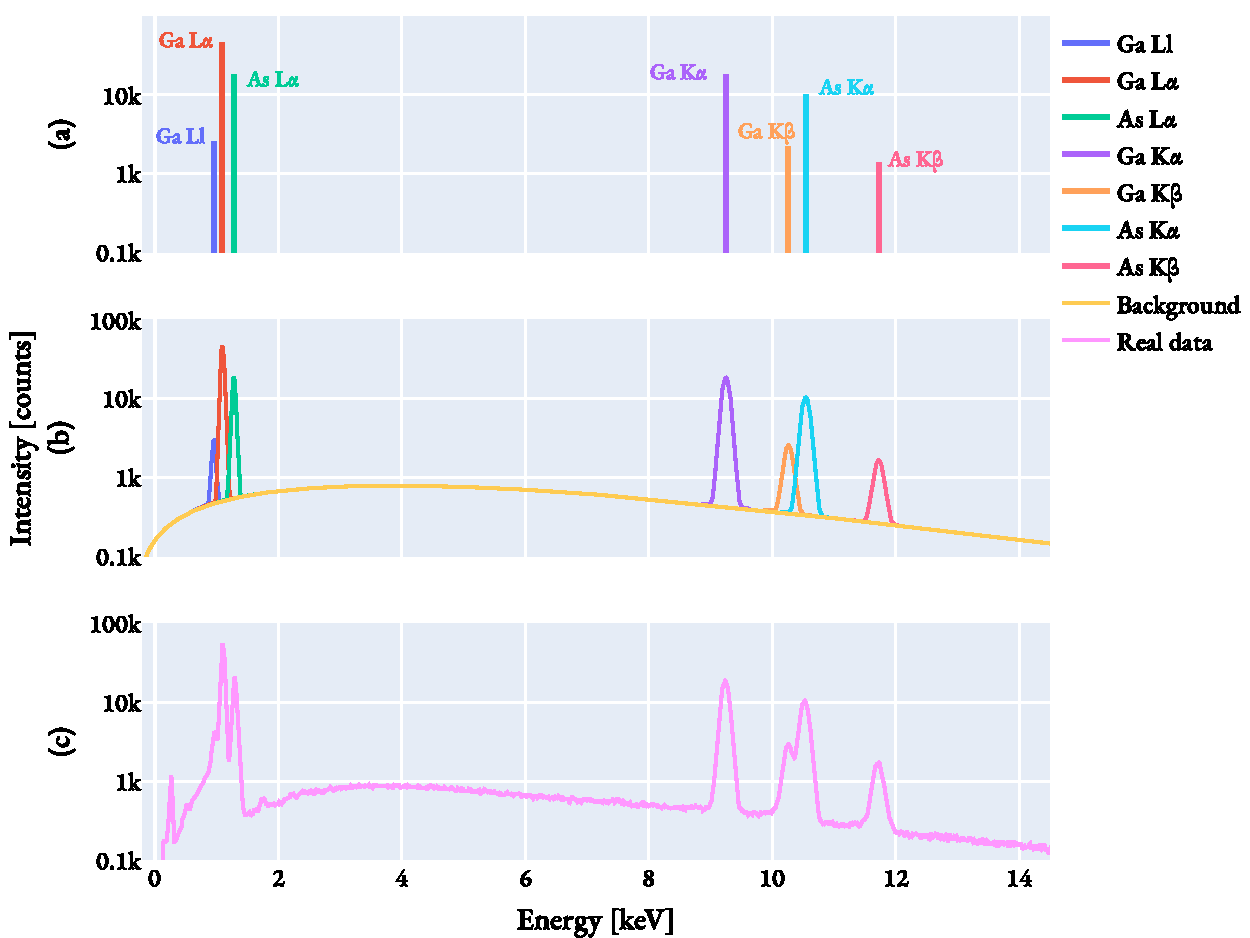
\includegraphics[width=0.99\linewidth]{figures/eds_theoretical2realSpectrum.pdf}
    \caption{
        From theory to an observed spectrum.
        (a) a theoretical spectrum with only the characteristic lines, (b) lines broadened to peaks on a background, and (c) an observed spectrum.
        The spectrum is of GaAs, and the peak names are annotated in (a).
        The background in (b) is modelled as a polynomial function of the energy.
        (c) show the noise peak and a small internal fluorescence peak at 1.74 keV (Si K$\alpha$).
        \brynjar{TODO: mark artifacts by arrow}
    }
    \label{fig:eds_theoretical2realSpectrum}

\end{figure}


%
\begin{table}[p]
    \centering
    \caption{
        The line energies of the most relevant lines in this thesis.
        The energies and weights are from HyperSpy \cite{hyperspy_1.7.1}.
        The relative weights are the intensity relative to the strongest line in the group, i.e. L$\alpha$ or K$\alpha$.
    }
    \label{tab:theory:lineEnergies}
    \begin{tabular}{ccccc}
        Energy [keV] & Element & Line          & Relative weight \\
        \hline
        0.277        & C       & K$\alpha$     & 1.00            \\
        0.525        & O       & K$\alpha$     & 1.00            \\
        0.957        & Ga      & Ll            & 0.05            \\
        1.098        & Ga      & L$\alpha$     & 1.00            \\
        1.120        & As      & Ll            & 0.05            \\
        1.125        & Ga      & L$\beta$$_1$  & 0.17            \\
        1.195        & Ga      & L$\beta$$_3$  & 0.05            \\
        1.282        & As      & L$\alpha$     & 1.00            \\
        1.317        & As      & L$\beta$$_1$  & 0.17            \\
        1.386        & As      & L$\beta$$_3$  & 0.05            \\
        1.740        & Si      & K$\alpha$     & 1.00            \\
        1.839        & Si      & K$\beta$      & 0.03            \\
        3.189        & Sb      & Ll            & 0.04            \\
        3.605        & Sb      & L$\alpha$     & 1.00            \\
        3.844        & Sb      & L$\beta$$_1$  & 0.43            \\
        3.886        & Sb      & L$\beta$$_4$  & 0.09            \\
        3.933        & Sb      & L$\beta$$_3$  & 0.15            \\
        4.101        & Sb      & L$\beta$$_2$  & 0.16            \\
        4.349        & Sb      & L$\gamma$$_1$ & 0.06            \\
        4.600        & Sb      & L$\gamma$$_3$ & 0.03            \\
        9.252        & Ga      & K$\alpha$     & 1.00            \\
        10.264       & Ga      & K$\beta$      & 0.13            \\
        10.544       & As      & K$\alpha$     & 1.00            \\
        11.726       & As      & K$\beta$      & 0.15            \\
        26.359       & Sb      & K$\alpha$     & 1.00            \\
        29.726       & Sb      & K$\beta$      & 0.15
    \end{tabular}
\end{table}



\begin{table}[phb]
    \begin{center}
        \caption{
            Definitions for various terms related to the generation of X-rays, \cref{theory:xray_formation}.
        }
        \renewcommand*{\arraystretch}{1.4}
        \label{tab:xray_generation}
        \begin{tabular}{p{3cm}p{11.6cm}}
            \hline
            \textbf{Name}                        & \textbf{Definition}                                                                                                                                                                                         \\
            \hline
            % Goldstein	&	The textbook on SEM and EDS in SEM. Refered to by almost all of the references in this work, and the co-authors have published many of the studies refered to.	\\
            Characteristic X-ray                 & An X-ray photon originating from a certain orbital transition, with a very specific energy.                                                                                                                 \\
            Incident (electron) beam             & The incident electron beam from the EM, which ionize the atoms and produce the signals detected. See  \cref{fig:characteristic_xray_formation}.                                                             \\
            Inner shell electron                 & The electron in the orbital closest to the atomic core. This is the electron that is ionized. See  \cref{fig:characteristic_xray_formation}.                                                                \\
            Outer shell electron                 & The electron from the outer orbital which is relaxed into the hole left by the ionized electron. See  \cref{fig:characteristic_xray_formation}.                                                             \\
            Atomic number, Z                     & The atomic number of the element.                                                                                                                                                                           \\
            Critical ionization energy, $E_C$    & The energy required to ionize the element of interest. Dependent on Z and the orbital to excite.                                                                                                            \\
            Secondary fluorescence               & When an X-ray photon loose energy to ionize another atom, thus creating a new characteristic X-ray.                                                                                                         \\
            Absorption edge                      & The energy where $\mu_\rho$ abruptly increase, because the energy is slightly above the $E_C$, and incoming electrons can thus ionize the respective line.  See \cref{fig:background_absorptionEdgeSi}.     \\
            Fluorescence yield, $\omega$         & The ratio of characteristic X-rays to Auger electrons, which change for the ionized shell ($\omega_K$ > $\omega_L$ > > $\omega_M$) and tend to increase with Z.  See  \cref{fig:theory:fluorescence_yield}. \\
            Ionization cross-section, $\sigma_T$ & The probability of the ionization at a certain energy for a given line. See \cref{eq:ionizationcrosssection}                                                                                                \\
            Selection rules                      & Quantum mechanical rules which specifies the allowed orbital transitions for the relaxing electron. See \cref{eq:theory:selectionrules}.                                                                    \\
            Background X-rays                    & X-rays generated by deacceleration of the electrons in the Coulomb fields of the atoms, which is noise in the analysis. See \cref{fig:background_xrays}.                                                    \\
            Relative weight                      & The relative intensity of a line compared to the strongest line in the group.                                                                                                                               \\
            Line vs. peak                        & In this work, line generally refers to the characteristic X-ray, while peak refers to the broadened signal in the spectrum.                                                                                 \\
            \hline
        \end{tabular}
    \end{center}
\end{table}






















\clearpage

\section{Scanning electron microscopy (SEM)}
\label{theory:sem}

% intro
This study involves the use of a controllable nanometer-scale electron beam to generate an X-ray spectrum for analyzing the composition of small volumes, primarily a SEM equipped with an EDS detector.
In SEM the electron beam has energies in the range 1-30 kV and bulk specimens are usually analyzed.
In TEM the electron beam has energies in the range 100-300 kV and thin specimens (> 100 nm) are usually analyzed.
The differences for EDS analysis will be addressed at the end.
Electron microscopes are often equipped with an EDS detector to provide analytical capabilities that complement imaging and diffraction analyzes.
This section provides a brief overview of how the electron beam is created and controlled in the electron microscope, as well as information on electron-matter interaction, imaging detection and image contrast in SEM.
If not stated otherwise, this section on SEM is based on Goldstein \cite{goldstein_scanning_2018}.

A summary of terms in the section is provided in \cref{tab:sem}.


\subsection{Electron beam generation and control}
\label{theory:sem:setup}

% Creating the electron beam
A schematic of a SEM is shown in \cref{fig:SEM_setup}. The \textbf{electron gun} is the source of the electron beam, where electrons are emitted with high kinetic energy by a high voltage.
Currently, the field emission guns are standard because they produce a brilliant beam compared to thermoinonic filament, and thereby high signal and good spatial resolution with the possibility of sum nm spot size.
The emittance of the electron gun is controlled by the user with the beam current and the accelerating voltage.
The acceleration voltage, or the beam energy $E_0$, is typically in the range of 1-30 keV.
The beam current is typically in the range of 0.01-10 nA.


% figure/SEM_setup.png
\begin{figure}[ht]
    \centering
    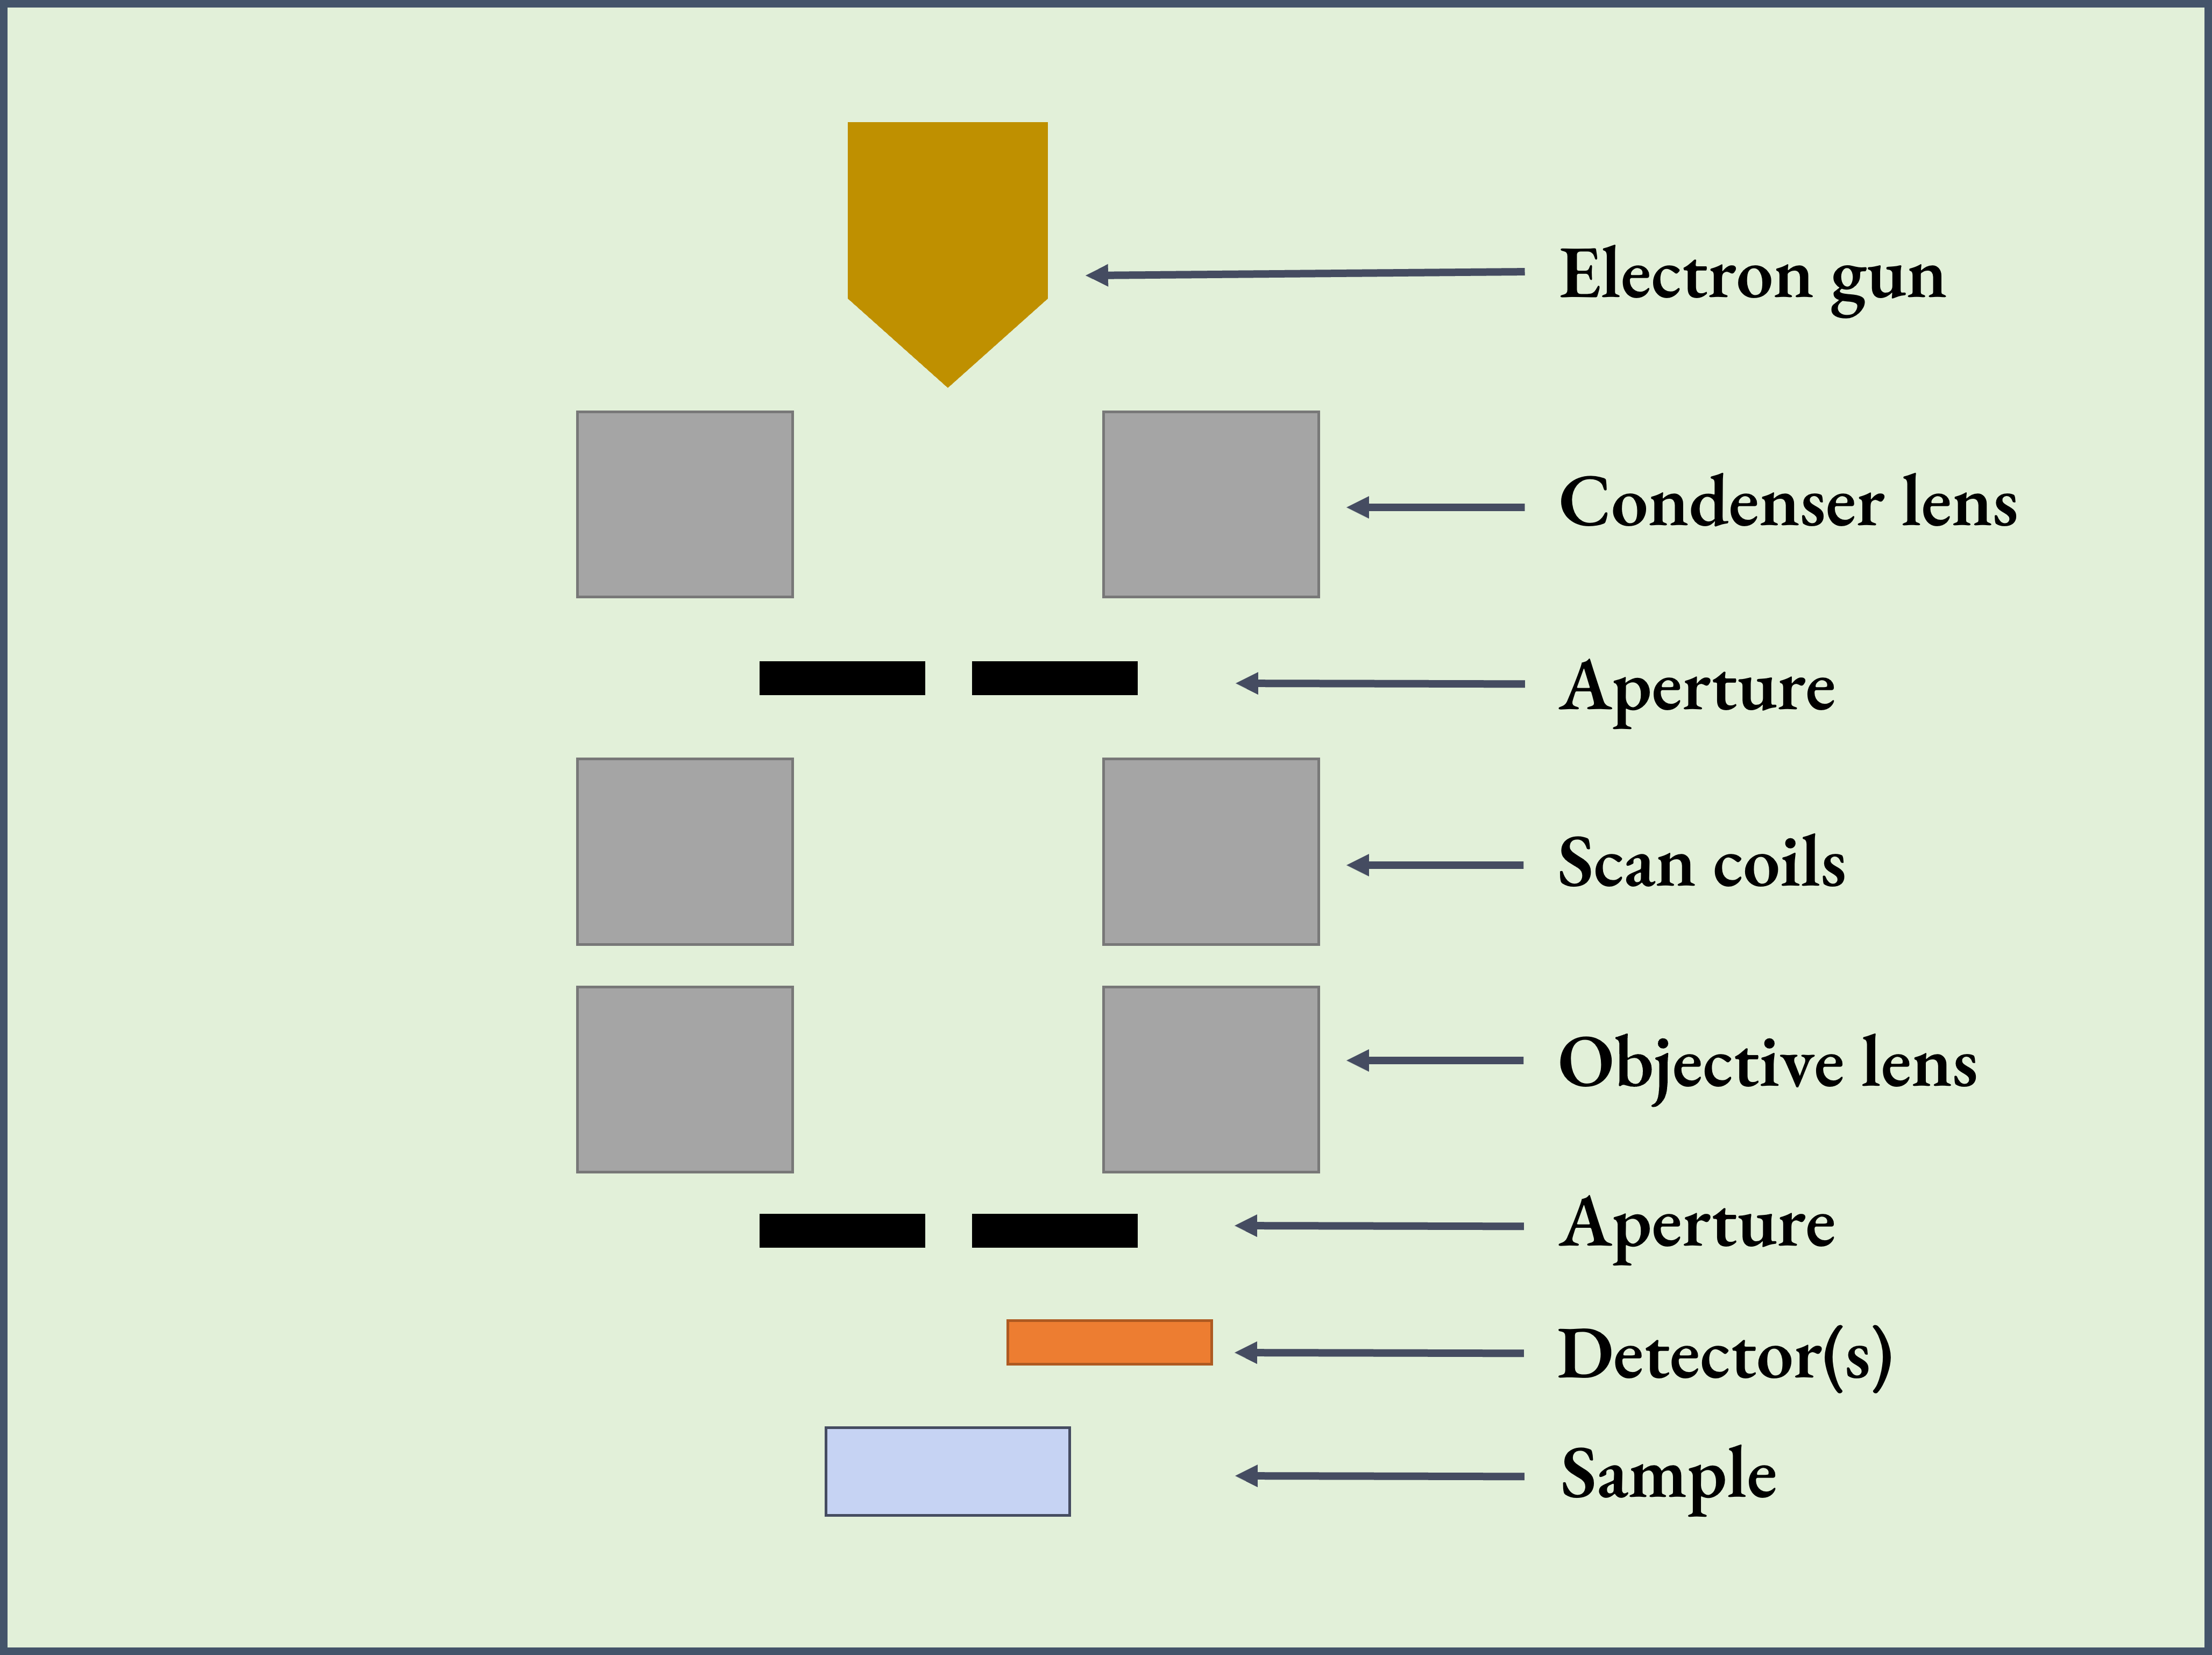
\includegraphics[width=0.8\linewidth]{figures/SEM_setup.png}
    \caption{
        Illustration of the main parts in an SEM.
    }
    \label{fig:SEM_setup}
\end{figure}


% Controlling the electron beam with lenses
The electron beam is shaped and controlled by \textbf{electromagnetic lenses and apertures}.
A narrower beam is wanted for higher resolution, as both the probe size is smaller and the electrons closer to the center of the beam axis have fewer aberrations \cite{goodhew_2001}.
The apertures are a physical barrier that limits the beam size.
A smaller probe with fewer aberrations is better for high resolution details, but the signal is also reduced as there are fewer electrons in the probe.
The condenser lenses are used to control the spot size and the shape of the beam.
The final lens, the objective lens, fine-tunes the beam's focus on the sample surface.
If the specimen is magnetic, the beam can be affected by the magnetic field of the sample.
Stigmator are used to prevent the beam from being elliptical.
The user of the microscope adjusts the focus with the objective lens and roundness of the probe with the stigmator.
The probe size can also be adjusted by changing the working distance, which is the distance between the objective lens exit and the sample surface.
Short working distances can produce the smallest probes, but they limit the depth in imaging and possibly the amount of signal that reaches the EDS detector.


% the scanning coils, with a raster scan illustration
The position of the probe on the surface is controlled by the \textbf{scanning coils} located between the condenser and objective lenses.
These scanning coils are used to create a raster scan, where the probe is moved in a grid pattern across the sample surface.
In each position the detector(s) register a signal, which is put together to form an 2D image, where each probe position corresponds to a pixel in the image.
The raster scan is visualized in \cref{fig:sem_rasterscan}.
The figure shows a probe that is moved in a grid pattern across the sample surface, resulting in a 2D image with different intensities.
The EDS signal is chosen for the visualization in the figure, but the same principle with the image being an intensity map applies to other signals like secondary electrons.
Scanning the probe over a smaller area, with equally many pixels, results in a zoomed in image.
The scan is controlled by the dwell time, which is the time spent recording a signal in each position.
Higher dwell times giving higher signal intensity which usually results in a clearer image, but long dwell time can result in beam damage issues, e.g. carbon deposition on the sample surface.
% A wave generator can generate a saw-tooth profile that rasterizes the probe across the sample. 

% figure/SEM_raster.png
\begin{figure}[ht]
    \centering
    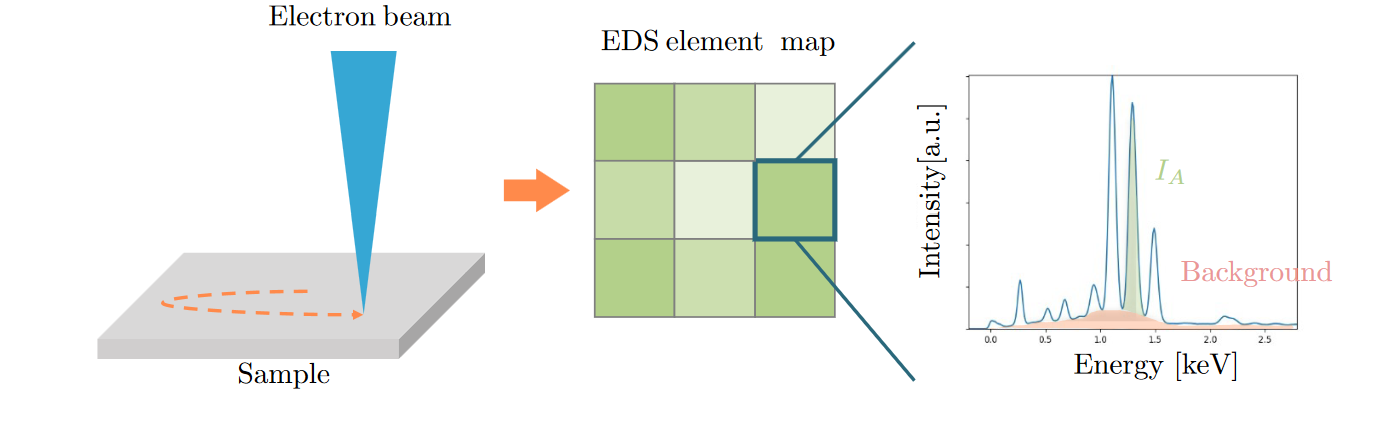
\includegraphics[width=0.8\linewidth]{figures/SEM_raster.png}
    \caption{
        Illustration of a raster scan in an SEM.
        The probe is moved in a grid pattern across the specimen surface, and the detector(s) register a signal for each position.
        The signal intensity recorded in each position corresponds to the color of the pixel in the resulting 2D image.
        This figure is adapted from Skomedal \cite[Fig. 2.14]{skomedal_improving_2022}.
    }
    \label{fig:sem_rasterscan}
\end{figure}






\subsection{Signals and image formation}
\label{theory:sem:sem_signals}

% The different signals
The interaction between the electron beam and the specimen results in a range of signals, illustrated in \cref{fig:interaction_volume}.
% The different signals illustrated in \cref{fig:interaction_volume} are generated by different interactions of the electron beam with the specimen.
The signals are briefly described in the following paragraphs, and they are: Auger electrons, secondary electrons, backscattered electrons, characteristic X-rays and background X-rays.
The detected signals are determined by what type of detector is used.



% The interaction volume
When the electron beam hits the specimen, a range of interactions can happen. % being the source of the different signals in the SEM.
The different signals originate from different depths in the specimen, illustrated by the \textbf{interaction volume} in \cref{fig:interaction_volume}.
The interaction volume has a droplet shape showing where the different signals are formed and emitted from.
The depth of formation is dependent on the beam energy, as higher $E_0$ makes the electron beam penetrate deeper into the specimen.
When a signal is formed inside the specimen, the signal can be absorbed or scattered within the specimen before it is detected.
The probability of the escape of a signal is dependent on the energy of the signal, the depth of generation, and the properties of the elements in the specimen.
Higher energy signals penetrate longer, and can thus escape from deeper inside the specimen.
Both the density of the specimen and the atomic number of the elements in the specimen affect the probability of escape.
Additionally, the geometry of the specimen can affect the probability of escape.
\cref{fig:interaction_volume} is annotated with schematically estimates for the depth of origin of the different signals detected \cite{goldstein_scanning_2018,hollas_modern_2004}.
Hence, the specimen geometry can be important.
% As the samples in TEMs are around 100 nm, the interaction volume in TEM samples is very small, resulting in less signals generated, as a larger portion of the beam passes through the sample without generating signals.
% Ton skriver om setningen over: Maybe more clear to delete this here, first describe SEM and later TEM (+ refering back)
A more accurate escape depth and interaction volume can be achieved by using a Monte Carlo simulation, which is a computer simulation of the interaction of the beam with the sample \cite[Ch. 4.3.4]{goldstein_scanning_2018}.
\cref{fig:montecarlo_BSE} shows an example of Monte Carlo simulations in a bulk samples for different materials.
Note that SE yield and interaction volume depends on Z the beam energy.


% figures/interaction_volume.png
\begin{figure}[ht]
    \centering
    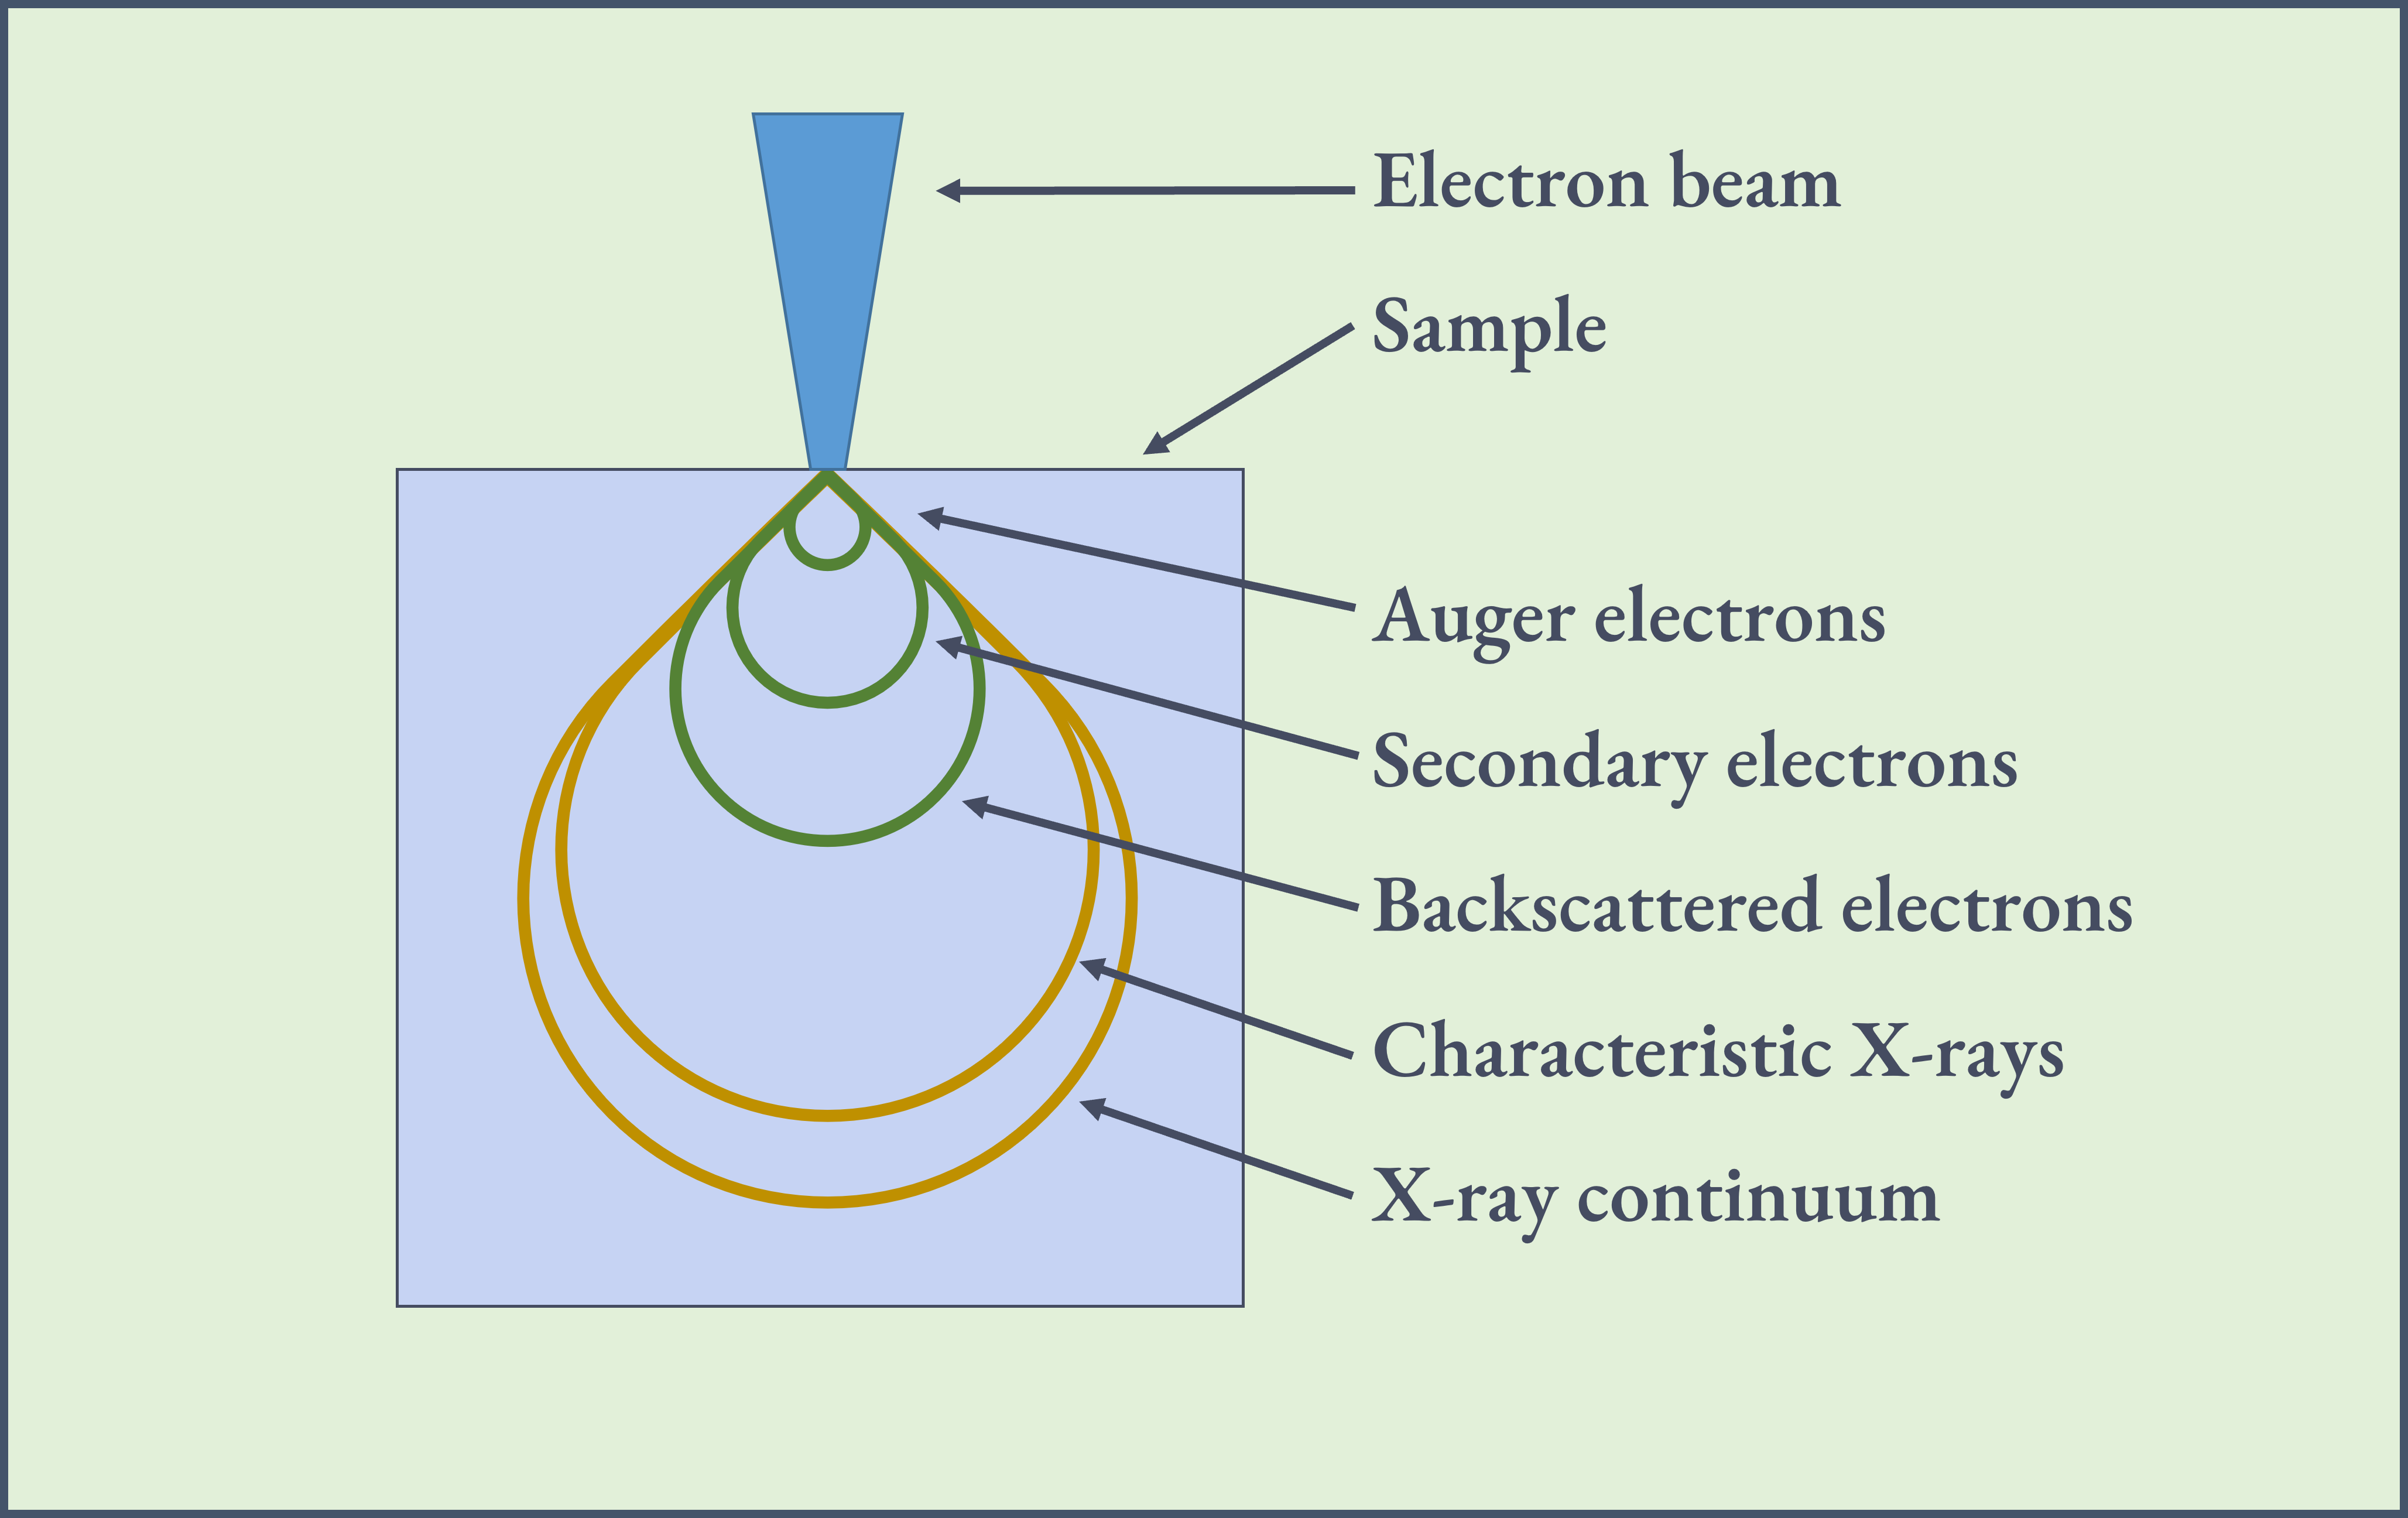
\includegraphics[width=0.9\linewidth]{figures/interaction_volume.png}
    \caption{
        Illustration of the interaction volume in a bulk sample, which is the regions from where the generated signals can escape the sample.
        The blue signals are electrons and the green signals are X-rays.
        The given depths are very rough estimates \cite{goldstein_scanning_2018,hollas_modern_2004}, as the depth strongly depends on the beam energy and the elements in the sample, as well as the geometry of the sample.
    }
    \label{fig:interaction_volume}
\end{figure}



% Auger electrons
\textbf{Auger electrons} are emitted in the following way: an incident electron ionizes an inner shell electron of an atom, which makes an outer shell electron relax to the hole in the inner shell, and the energy difference is used to emit another electron, which is an Auger electron.
Auger electrons have very low specific energy and are only detectable from the surface of the specimen, having an escape depth around 2 nm \cite{hollas_modern_2004}.


% Secondary electrons
\textbf{Secondary electrons (SE)} are formed by inelastic scattering between incident beam electrons and valence electrons of the atoms in the specimen.
The weakly bound valence electron is knocked out of the atom, but with low kinetic energy from 0 to 50 eV.
A plot of the distribution of the kinetic energy of the SE is shown in \cref{fig:SEM_SE_spectrums}, which is from a Cu sample with a 1 keV beam.
Since the SE have low energy, they cannot travel far inside the sample before they are absorbed or scattered, and the SE signal is thus used to get topological information.
If the beam is hitting the surface near an edge, the SE can escape at the edge, giving topological contrast.


% Backscattered electrons
\textbf{Backscattered electrons (BSE)} are from elastic scattering between incident beam electrons and atoms, where the scattering results in a reversed trajectory and thus making the incident electrons escape up through the sample surface.
The scattering process is interactions with the orbitals and the nuclei of the atoms, and since the BSE are the incident electrons, their kinetic energy is in the keV range.
Monte Carlo simulations shown in Goldstein \cite[Fig. 2.16 b]{goldstein_scanning_2018} show that more than half of the backscattered electrons in carbon retain more than 50\% of the initial energy of the incident beam electrons.
Atoms with higher atomic number have more protons and more electrons, giving them a higher probability of the scattering process, and thus making the BSE signal proportional to the atomic number, Z, of the atoms.
Thereby BSE images can give a fast and rough qualitative overview of the composition distribution.
As the BSE signal originates from deeper inside the sample, the topological information is limited.
\cref{fig:montecarlo_BSE} show Monte Carlo simulations with a 20 keV beam energy on C, Si, Cu, and Au.
The figure show that a higher Z gives more BSE, marked as red lines.
Additionally, the figure show that the size of the interaction volume is dependent on Z too, as all the scatterings are more concentrated in (d) with Au.
The blue lines are electrons which have had all their energy absorbed within the specimen.
In addition to the three types of electron signals, the beam interaction can also create X-ray photons.


\brynjar{Insert SE and BSE images of C-film on Cu-grid with Ga. Topology and Z-contrast.}


% Characteristic X-rays and background X-rays
Formation of \textbf{characteristic X-rays} are covered in detail in \cref{theory:xray_formation:characteristic}.
In short, formation of characteristic follow the same principle as Auger electrons, but the energy difference between the outer and inner orbital is used to emit X-rays instead of electrons.
Typical escape depths for X-ray signals are around 4000 nm \cite{hollas_modern_2004}, but the variations are large.
The escape depth depends on the energy of the photon and the density of the sample.
% \brynjar{Mention Li escape depth in range of tens of nm? Keith Thompson: Is Energy Resolution Still an Important Specification in EDS?} % Ton: nei
% The lower energy X-rays from Li (Z=3) have a shallow escape depth of only 
% the absorption in the sample makes the escape depth of light elements shallow. Eg. Li have an escape depth of only a few tens of nm (Keith Thompson, Is Energy Resolution Still an Important Specification in EDS?)
Lastly, the \textbf{background X-rays} are formed by the deacceleration of the incident beam electrons because of the Coulomb fields of the atoms in the specimen, and this deacceleration of charged particles emits photons \cite{notaros_electromagnetics_2010}.
The background X-rays are white noise, giving no information about the sample, and is generated in the whole interaction volume.



%figures/SEM_montecarlo_BSE.pdf
\begin{figure}[ht]
    \centering
    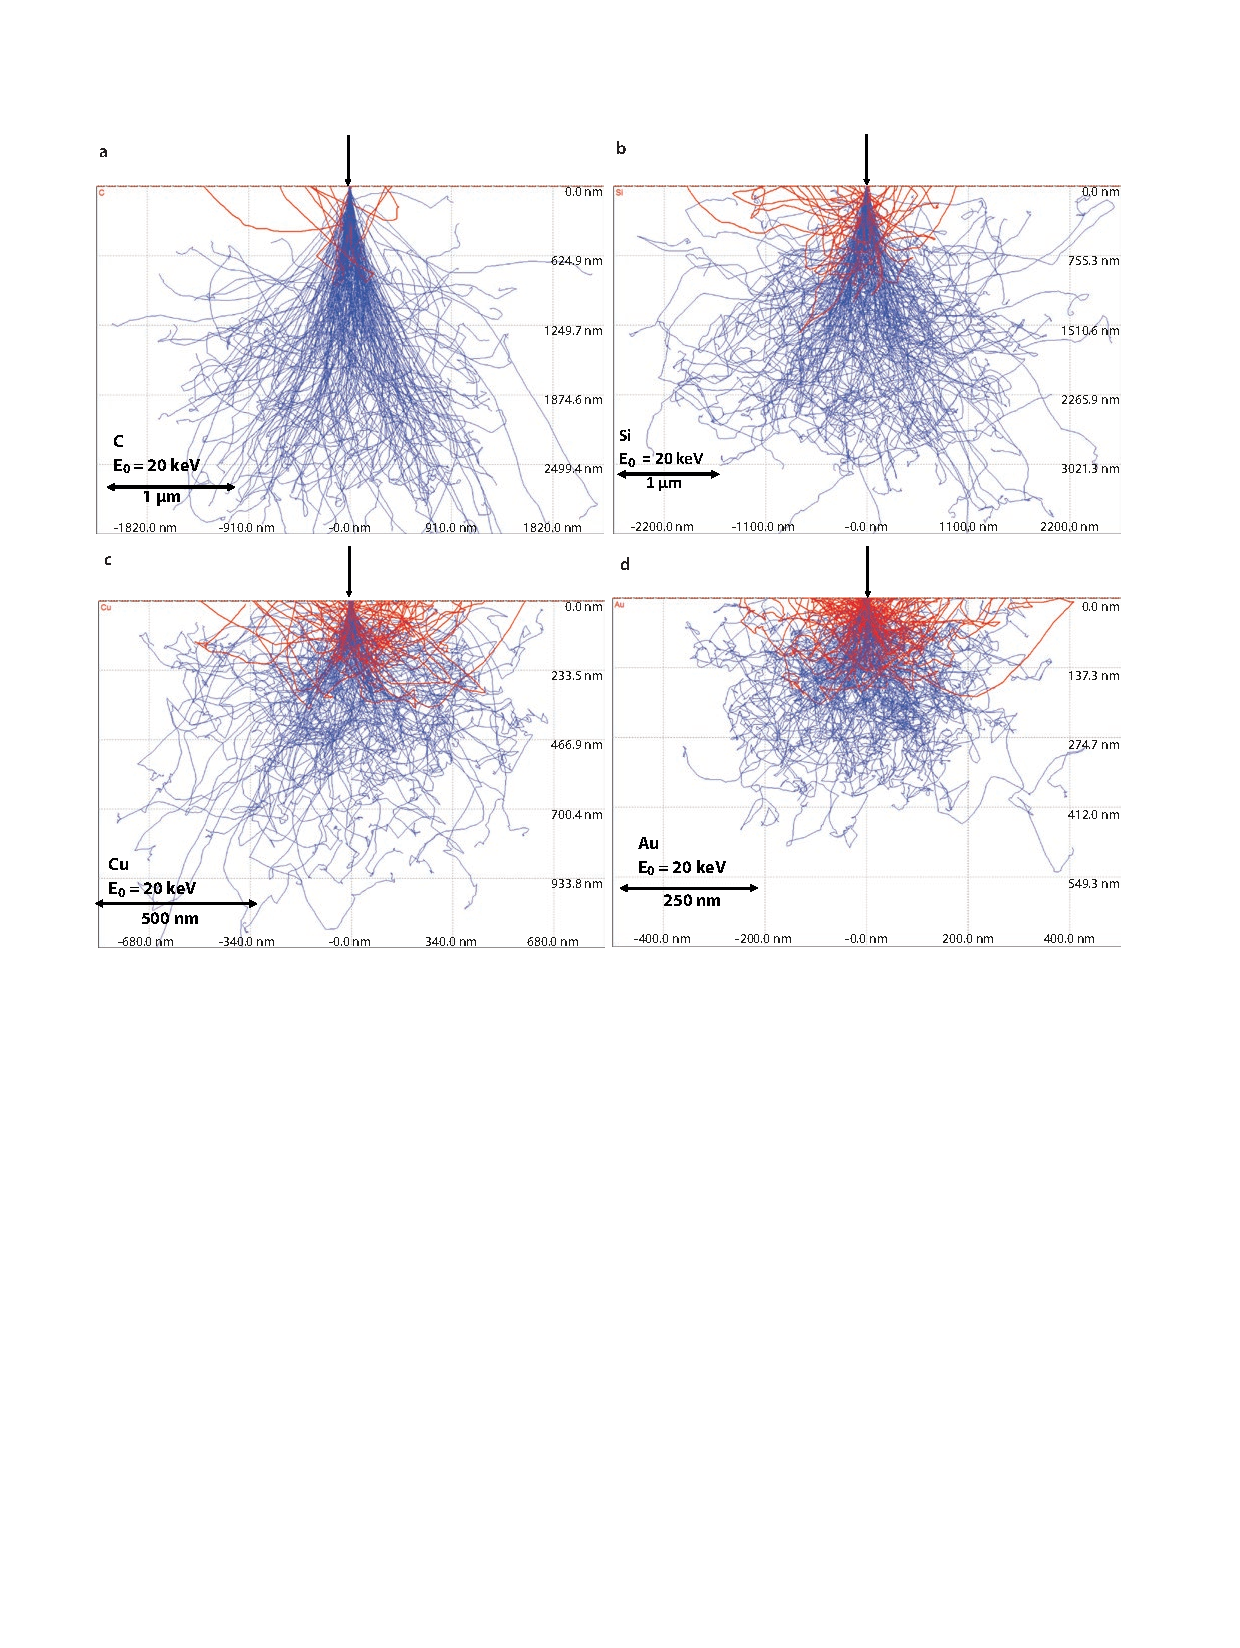
\includegraphics[width=0.8\linewidth]{figures/SEM_montecarlo_BSE.pdf}
    \caption{
        Monte Carlo simulation of the interaction volume in C, Si, Cu, and Au with 20 keV beam energy.
        The red lines mark the incident electrons with reversed trajectory, which are the BSE.
        The figure is adapted from Goldstein \cite[Fig. 2.2]{goldstein_scanning_2018}.
    }
    \label{fig:montecarlo_BSE}
\end{figure}


% The absorption of signals generated
The signals generated in the interaction volume can be \textbf{absorbed or scattered within the specimen}.
For example, secondary electrons can be generated near the surface by BSE, and are then called SE$_2$.
The SE with topological contrast (from the targeted area) are called SE$_1$.
The SE$_2$ signal carries the same information as the BSE signal, since the amount of SE$_2$ is proportional to the amount of BSE.
An SE signal generated from a BSE hitting something in the chamber is called a SE$_3$ signal, and SE signal from pre-specimen sources like the final aperture is called SE$_4$.
The final SE image can be a combination of all the SE classes.
The SE detector can be optimized, for example with  in-lens configuration, to only detect SE$_1$ and thereby give a better spatial resolution.
Other examples of signal absorption is the generated X-ray strays due to fluorescence, which is covered in \cref{theory:eds:artifacts}.


% Detection of the signals as spectra
While a range of signals are formed by the interaction of the beam with the specimen, \textbf{the observed signals} depend on the detector used.
One type of SE detectors are the Everhart-Thornley detector \cite{everhart_detector1960}, which combines the SE signal with the BSE signal to get both topological and compositional contrast in the same image.
BSE detectors can be annular solid state detectors or in-lens detectors.
BSE imaging or combination of BSE and SE can be used to get initial compositional information before detailed quantitative EDS analysis.
EDS detectors are covered in detail in \cref{theory:eds}.
The signal from all types of detectors can be viewed as a spectrum, where the intensity of the signal is proportional to the number of electrons or X-rays detected.
A SE image is the 2D representation of a set of spectra, where each pixel is a 1D spectrum with the number of SE electrons detected as a function of energy.
In a 2D image, the intensity of a pixel is proportional to the sum of the number of electrons detected on that probe position.
\cref{fig:SEM_SE_spectrums} show what the spectrum from a single pixel in a SE image would look like.
The same is true for BSE images, only with a higher energy range.
Both SE and BSE detectors are counting the number of electrons detected, and the energy of the electrons is not used.
An electron microscope can be fitted with an electron spectrometer to measure the energy of the electrons, but this is not common as it requires a more complex detector design than counting detectors.
However, in EDS detectors the signal is recorded in each pixel as a digital histogram of the energy of the detected X-rays, making a spectrum map.
This allows for the creation of a 2D map of the elemental composition of the sample, as specific elements can be given colors in the image.
This is a very powerful tool for the analysis of samples, and is covered in detail in \cref{theory:eds}.
EDS spectra can also be recorded as a 1D spectrum from a point on the sample.

% figures/SEM_SE_spectrums.png
\begin{figure}[ht]
    \centering
    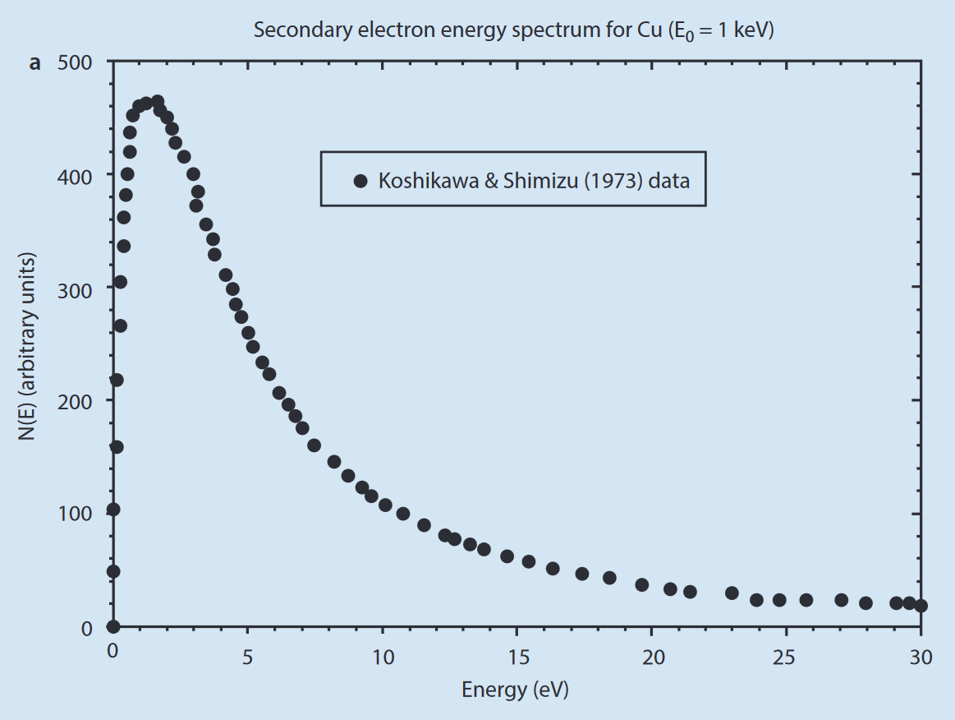
\includegraphics[width=0.8\linewidth]{figures/SEM_SE_spectrums.png}
    \caption{
        The figure shows the spectrum from a single pixel in a SE image.
        The specimen is Cu, and the incident beam energy is 1 keV.
        Similar spectrum would be recorded in a BSE image, but with peaks at different energies for the different elements.
        Normal SE and BSE images only record the sum of the registered electrons, and not the energy of the electrons.
        The figure is adapted from Goldstein \cite[Fig. 3.1 a]{goldstein_scanning_2018}, which use data from \cite{koshikawa_SE_spectrum_1973}.
    }
    \label{fig:SEM_SE_spectrums}
\end{figure}


\subsection{Note on transmission electron microscopy}
\label{theory:sem:tem}

There are several similarities between the SEM setup described above and TEM in scanning mode.
Both setups use lenses to form a fine probe that is rastered over the sample using scanning coils.
However, in the present work, the focus is mostly on SEM EDS, and the TEM setup is only briefly introduced, with a focus on the relevant differences to SEM EDS.
Firstly, the beam energy in TEM is higher (100-300 kV vs 1-30 in SEM), which can affect the likelihood of X-ray line creation.
Secondly, to transmit electrons, the specimen in TEM is thin (<100 nm), resulting in higher spatial resolution due to a smaller interaction volume.
The interaction volume in a bulk SEM specimen is illustrated in \cref{fig:interaction_volume}, but as the thickness of TEM specimen are in the nanometer range, the interaction volume is severely reduced.
This reduced interaction volume also decreases the likelihood of absorption and fluorescence, simplifying calculations and avoiding corrections.
However, a thinner specimen produces less signal and can result in a poorer signal-to-noise ratio.
These two aspects are the key differences, and TEM image formation is not discussed further in this work.



\begin{table}[phb]
    \begin{center}
        \caption{
            Definitions for various terms related to scanning electron microscope, \cref{theory:sem}.
        }
        \renewcommand*{\arraystretch}{1.4}
        \label{tab:sem}
        \begin{tabular}{p{4cm}p{10.6cm}}
            \hline
            \textbf{Name}                       & \textbf{Definition}                                                                                                       \\
            \hline
            Electron gun                        & The source of the electron beam.                                                                                          \\
            Beam energy, E$_0$                  & The voltage applied that accelerates the electrons in the beam.                                                           \\
            Beam current, I$_\textnormal{beam}$ & The current used to heat the electron gun and emit electrons to the beam.                                                 \\
            Probe size                          & The cross-section of the electron beam when it hits the sample.                                                           \\
            Electromagnetic lenses              & The lenses which shape and control the electron beam in the column. Condenser lenses, scanning coils, and objective lens. \\
            Aperture                            & A physical barrier with a hole in the middle which allows only part of the signal to pass through.                        \\
            Interaction volume                  & The volume in the sample where the different signals originate from.                                                      \\
            Auger electrons                     & A signal of electrons emittet from the surface of the sample.                                                             \\
            Secondary electrons                 & A surface sensitive signal of electrons used to produce images of the sample.                                             \\
            Backscattered electrons             & Electrons which have had their trajectory reversed through the scattering processes. Sensitive to Z.                      \\
            \hline
        \end{tabular}
    \end{center}
\end{table}

















\clearpage


\section{Energy dispersive X-ray spectroscopy (EDS)}
\label{theory:eds}


% Ok to discus principle of detection using Si(Li). Have a figure. 

% But add SDD, and the details/differences that matter 

% Add here geometry sample-detector as it will affect your results (phenomena absorption you have to have in section 1 or 2). 

% Intro
Energy dispersive X-ray spectroscopy is a technique for the analysis of the elemental composition of a sample with high spatial resolution.
The EDS system is made up of the detector capturing incoming X-rays, the electronics converting the analogue signal to a digital signal, and the and the software on the computer to analyze the signal through plotting and quantification.
The output of an EDS analysis is either a spectrum or a spectrum map, where the spectrum is a histogram with the number of X-rays detected as a function of energy.
Even though the resulting spectrum appears to be acquired simultaneously at all energies, the spectrum is actually acquired one channel at a time.
This section covers first the hardware and the principles of EDS detectors, then the information in a spectrum, and finally user controlled parameters in the EDS analysis.
\cref{theory:eds_performance} covers parameters used to quantify the performance of the EDS system. %and the quality of a spectrum.
% based on Goldstein
This section is based on Goldstein \cite{goldstein_scanning_2018} and Jenkins \cite{jenkins_xrayspectroscopy}, if not stated otherwise.




\subsection{EDS detectors hardware}
\label{theory:eds:hardware}

% Ton: Det er noe fundamentele ting med EDS vi må akseptere. Kanksje det er bra å state i teori eller diskusjon. 
% Andre detaljer, som mye i EDS literatur, er basert på gamle teori. 
% Om nye SDD er det mye mindre publisert og selve teknologi utvikler seg

% how the detectors detect
Detecting X-rays is a three-step process illustrated in \cref{fig:detecting_xrays}, nowadays done with a silicon drift detector (SDD).
The older Si(Li) detectors have similar working principles, but are generally performing worse than SDD, where the Si(Li) detectors have lower counts and smaller solid angle, as well as being less practical due to the need of liquid nitrogen cooling.
However, parts of the literature is old and based on the Si(Li) detector, and thus both detector types is described below.
Both detectors are Si based diode-structures, where incoming X-rays ionize Si atoms, creating electron-hole pairs.
The number of electron-hole pairs proportional to the energy of the incoming X-ray, and hence the X-ray signal can be plotted as function of its energy.
The electron-hole pairs is driven by an electric field towards the contact points, where they are converted into a voltage signal and amplified by FET transistors.
Finally, the electronics assigns the voltage signal to a specific energy range, called a channel.
While the electronics is converting the voltage signal, the detector is shut down by the controlling software.
The time the detector is shut down is called dead time, and is discussed in \cref{theory:eds:user_controlled_parameters}.
Each voltage signal registered corresponds to one count in the given channel.
The width of a channel is usually set to 10 eV, thus the scale of most spectra is 10 eV per channel.
The number of channels in a spectrum is typically 1024 or 2048.
The number of counts stored in a channel is the signal intensity.
Details about the signal is covered in \cref{theory:eds:artifacts}.
\cref{tab:eds:hardware} summarize this section.


% figures/detecting_xrays.png
\begin{figure}[ht]
    \centering
    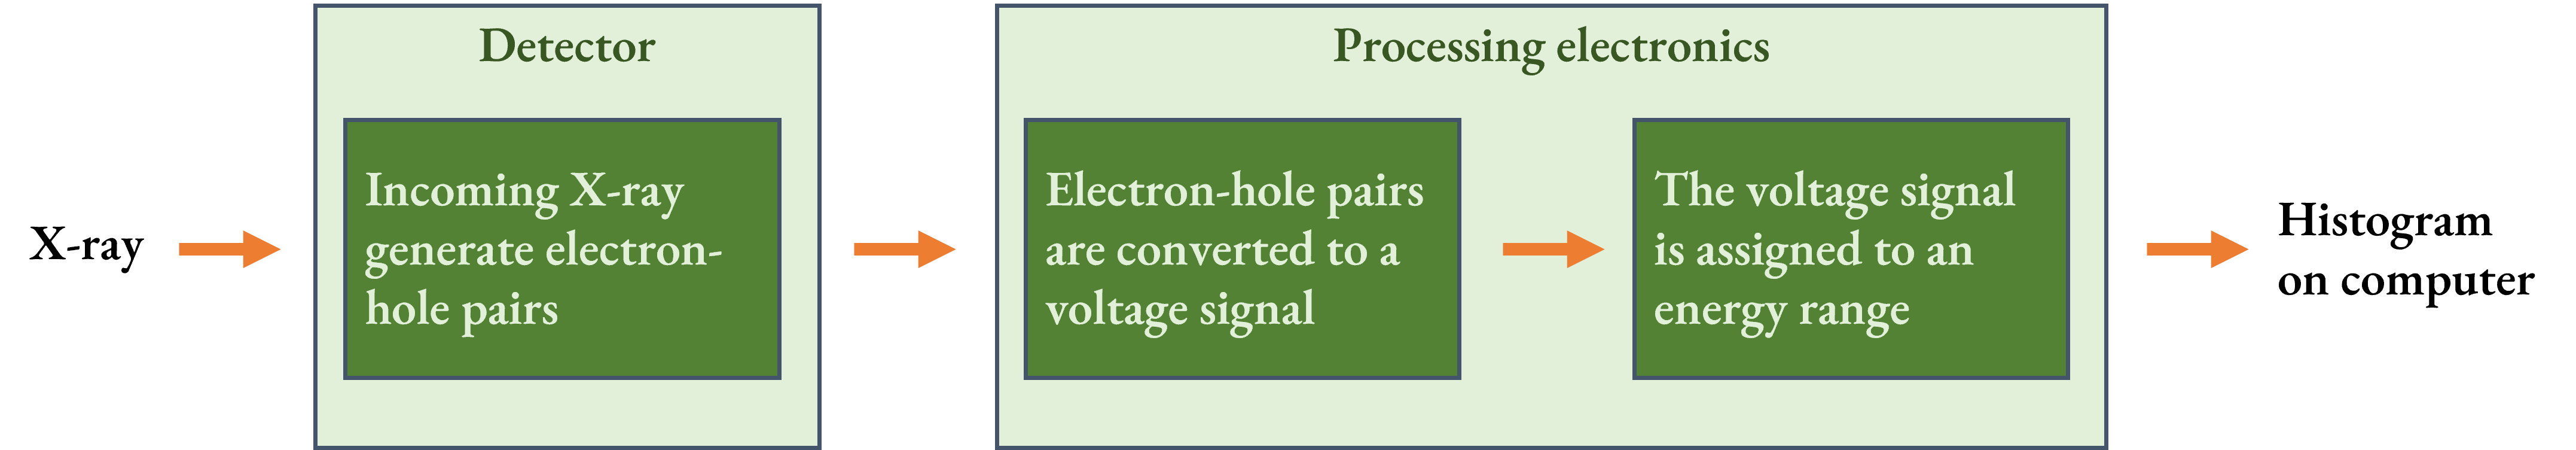
\includegraphics[width=0.9\linewidth]{figures/detecting_xrays.png}
    \caption{
        The figure shows the three-step process of detecting X-rays in EDS detectors.
    }
    \label{fig:detecting_xrays}
\end{figure}




% The Si(Li) detector
The Si(Li) detectors are silicon crystals drifted with lithium, with a p-i-n diode structure.
The generation of detectable electron-hole pairs happens in the thick intrinsic region.
The thinner n- and p-type regions are referred to as dead layers, because the electron-hole pairs generated there are not collected.
The layer where detectable electron-hole pairs are generated is called the active layer.
The thickness of the detector is typically 2-5 $\mu$m, which allows for a high detection efficiency at higher energies, since few X-rays are able to pass through the intrinsic layer without generating electron-hole pairs.
% \brynjar{Si dip is also there, because of the Si in the detector.} % Ignore?
When operating the detector, X-rays enter through the p-type end into the intrinsic region, where they have a high probability of being absorbed and thus ionizing a Si atom, which creates electron-hole pairs.
The number of electron-hole pairs created is proportional to the energy of the X-ray, since one pair requires 3.8 eV of energy.
A reverse bias over the detector makes the charge carriers drift towards the detector contact, where they are measured by the electronics after being amplified.
Since electron-hole pairs can be thermally excited, the detector is cooled to liquid nitrogen temperature to prevent this.
The liquid nitrogen cooling also prevents the lithium from diffusing under the field within the detector and reduce the electronic noise from the amplifiers in the electronics.

% The SDDs
The SDDs are also silicon crystals, but with a much thinner active layer and generally a different design.
A schematic of an SDD is shown in \cref{fig:eds_sdd}.
Incoming electrons pass through the collimator, which is an aperture that limits the angle which the X-rays can enter the detector.
The collimator limits detection of X-rays from other parts of the sample and the chamber.
The detector window is a barrier that maintains vacuum in the detector, usually made of beryllium or being polymer based.
Be windows strongly absorbs low energy X-rays, allowing only X-rays above Na to pass through, while polymer windows are transparent down to 100 eV, but are less robust.
Some detectors, especially in TEM, are windowless.
The sensor in SDDs is a thin layer of doped Si, with ring electrodes on the anode side.
The X-rays enter through the cathode side, ionize Si atoms, and create electron-hole pairs, which are drifted by the ring electrodes towards the center.
In the center of the backside is a small anode, where the electron-hole pairs are collected.
The anode is connected to a FET transistor which amplifies the voltage signal.
The signal is then sent to the electronics, where the pulse processor is converting the analogue signals to digital signals.
The digital signals are sent to the multichannel analyzer, which makes a spectrum from the digital signals.
The spectrum is then sent to the computer, where the user can analyze the spectrum.


% figures/EDS_SDD.png
\begin{figure}[pht]
    \centering
    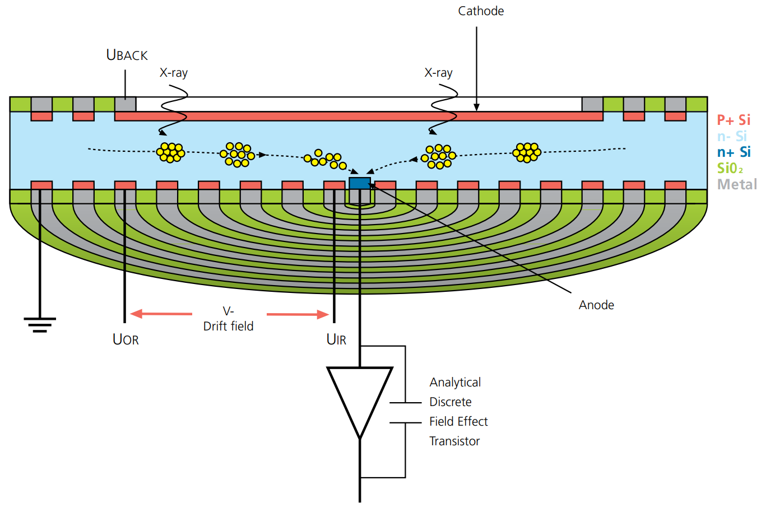
\includegraphics[width=0.89\linewidth]{figures/EDS_SDD.png}
    \caption{
        A schematic of the side view of a silicon drift detector (SDD).
        The collimator and window would be placed in front of the cathode.
        % The electronics are after the FET transistor.
        The figure is adapted from Oxford Instruments \cite{oxford_sdd_explained}.
    }
    \label{fig:eds_sdd}
\end{figure}



% SDD vs Si(Li) detectors
There are some key differences between the Si(Li) and SDD detectors. %, making the SDDs in general both better and more user friendly.
The cooling needed in the more modern silicon drift detectors (SDD) is not as strong as for the Si(Li) detectors. %, which is one of the differences between the detector types.
The SDDs need no more than a Peltier cooling (ca. -20 to -30\textdegree C), which is easy to operate and maintain.
The anode in the SDDs is just a small centerpiece, while in the Si(Li) detectors the anode covers the whole detector.
As the anode is smaller, the capacitance is lower and the voltage noise is reduced.
In SDDs the area of the active layer can be made bigger with a constant anode size, which keeps the capacitance constant. \cite{notaros_electromagnetics_2010}.
An increase in capacitance is not good, as it is limiting both resolution and throughput \cite[Ch. 16.3.9]{goldstein_scanning_2018}.
A bigger active area allows more counts per second, as it is increasing the solid angle, explained further down.
The lower voltage noise in SDDs allow both a cleaner signal and a shorter process time, because the pulse processor does not need to do signal averaging.
The shorter process time allow significantly higher count rates and high speed mapping.
High speed mapping is a key feature in SEM EDS, which is not available or less accurate in other X-ray analysis methods.
One of the drawbacks of the SDDs compared to the Si(Li) detectors, is the detector efficiency ($\varepsilon$), illustrated in \cref{fig:detector_efficiency}.
The lower efficiency of the SDDs is due to the thinner active layer, which allows high energy X-rays to pass through without generating electron-hole pairs.
% This effects begins around 6-9 keV, and the effect increase with higher energies.
% with origin in the thinner active layer, it that the SDDs allows more of the X-rays to pass through the active layer without generating electron-hole pairs, which lowers the detector efficiency.
% The decrease in detector efficiency begins around 6-9 keV, and the effect increase with higher energies, illustrated in \cref{fig:detector_efficiency}.


% figure/detector_efficiency_illustration.pdf
\begin{figure}[pht]
    \centering
    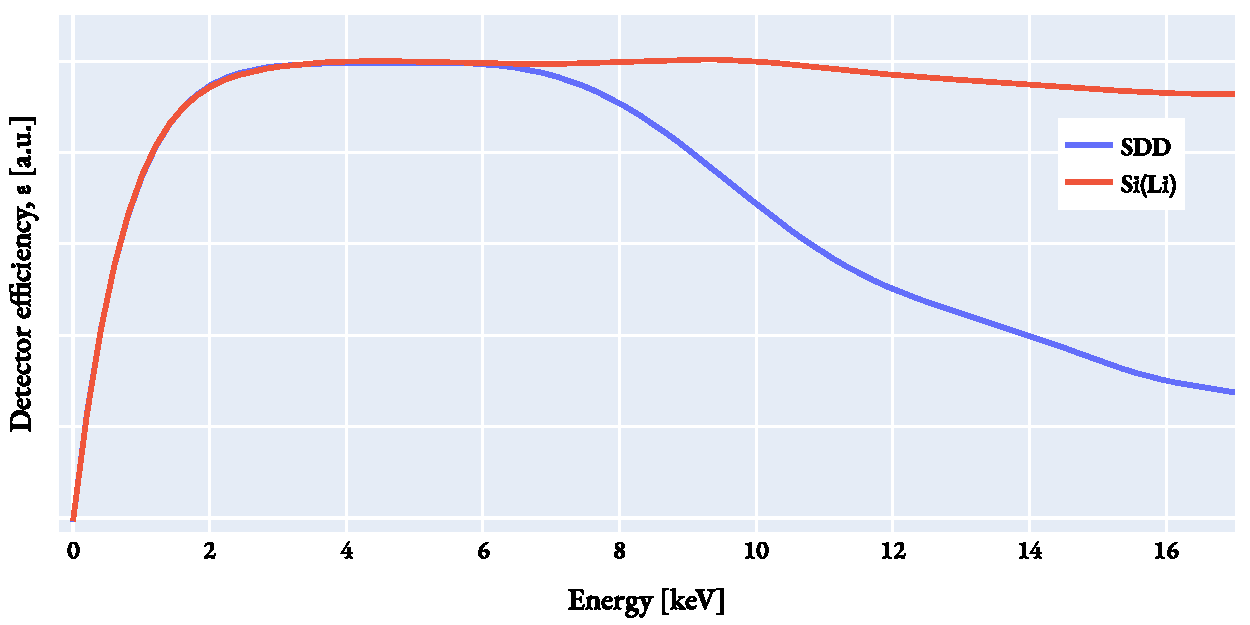
\includegraphics[width=0.8\linewidth]{figures/detector_efficiency_illustration.pdf}
    \caption{
        Illustration of the detector efficiency ($\varepsilon$) of a Si(Li) and an SDD, as a function of the X-ray energy.
        The efficiency of the SDDs decrease at higher energies because the active layer is thin, and thus high energy X-ray photons have a higher probability of passing through without creating an electron-hole pair.
        Figure adapted from \cite[Fig. 4655c]{liao2006practical}
        \brynjar{Consider an alternative source.}
        % Remake of \brynjar{find one, e.g. https://www.globalsino.com/EM/page4655.html}
    }
    \label{fig:detector_efficiency}
\end{figure}




% Geometry
The position of the detector affects the analysis, and the geometry around the detector is illustrated in \cref{fig:eds_geometry}.
The number of X-rays hitting the active area of the detector is dependent on the solid angle ($\Omega$) and take-off angle (TOA), which covers both tilt of the specimen and the detector.
The solid angle, $\Omega$, is an expression of the fraction of the sphere with radius from the center of the detector to the sample that the detector is covering.
\brynjar{TODO Comment from Ton: "In future work propose how to measure this out of the detected signal. I think you cannot do it practically at this stage."}
In \cref{fig:eds_geometry} the solid angle is marked as a yellow triangle, but in 3D it has a cone shape, measured in steradians.
The whole hemisphere above the surface of the sample has a solid angle of 2$\pi$ steradians, and the solid angle of the detector is the fraction of this hemisphere that is covered by the detector.
A bigger detector covers a bigger fraction of the hemisphere, and thus collects more X-rays.
$\Omega$ is the active area (A) of the detector divided by the square of r, the distance from the detector to the incident point of the probe on the specimen.
Moving the detector closer to the sample increases the solid angle, and thus the number of counts.
When the sample is in horizontal position, the TOA is equal to the elevation angle of the detector, which is typically between 35 and 40 degrees \cite{dtsaii_1_getting_started}.
Changing the tilt of the sample changes the TOA, and can increase intensity of the signal and reduce the path length in the specimen, and thereby reduce the absorption of the X-rays.
The azimuthal angle is marked as az in the figure, and is the position of the detector in the xy-plane, measured from the x-axis.
The azimuthal angle is important in the link between a SEM image and the corresponding EDS spectrum, as the azimuthal angle tells where the apparently X-ray illumination is coming from.
The working distance (WD) is the distance from the end of the SEM column to the sample, and is marked as WD in the figure.
The optimal WD is the height where the straight line of sight from the detector to the sample and the incident point of the probe on the sample coincide.
Both a too low and too high WD will limit the number of counts, and most EDS operating software specify an optimal WD for the detector.




% figure/EDS_geometry.png
\begin{figure}[ht]
    \centering
    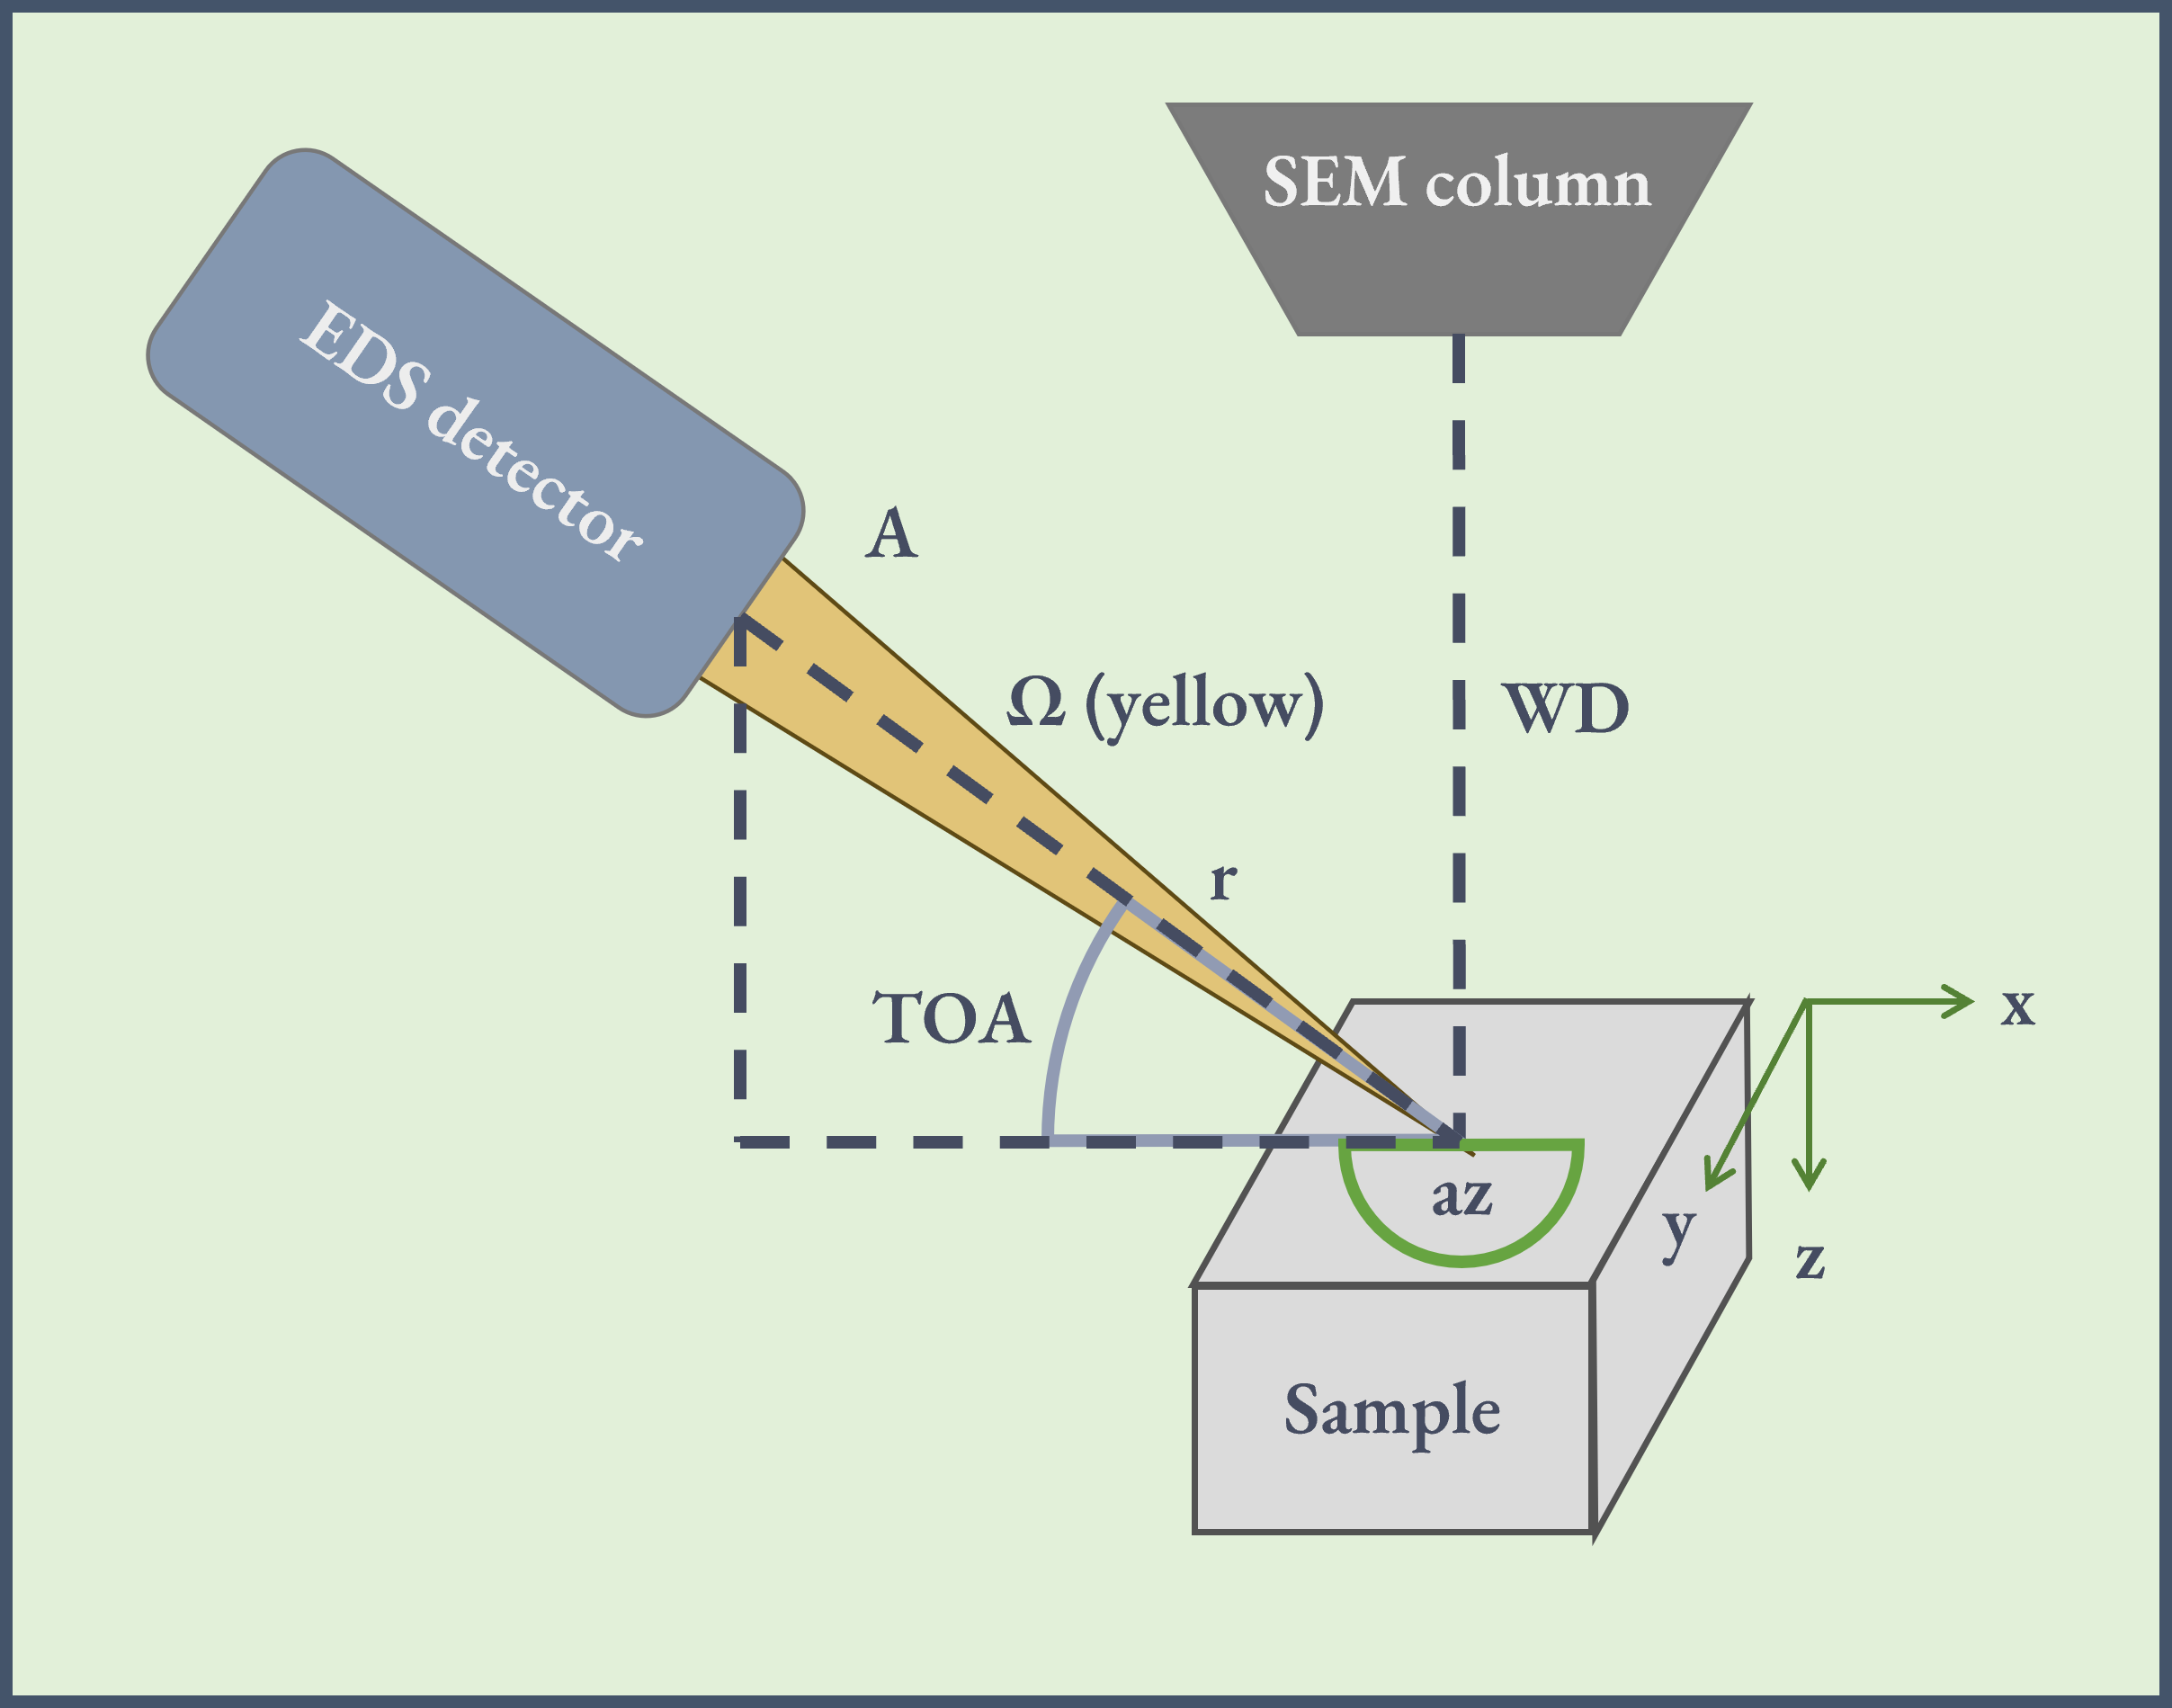
\includegraphics[width=0.6\linewidth]{figures/EDS_geometry.png}
    \caption{
        A schematic of the geometry of the sample and detector in EDS.
        The solid angle ($\Omega$) is a function of A and r, giving the fraction of the hemisphere above the sample that is covered by the detector.
        X-rays with trajectory outside the yellow triangle will not hit the detector.
        The TOA is take-off angle, WD is working distance, az is the azimuthal angle, A is the active area of the detector, and r is the distance from the sample to the detector.
    }
    \label{fig:eds_geometry}
\end{figure}






% Peak broadening due to electronics
One of the main drawbacks of the EDS is the poor energy resolution. %peak broadening due to the electronics.
The natural line widths of the X-ray lines treated in this work is around 10 eV, but the peak widths in EDS spectra are around ten times larger, as stated in \cref{theory:xray_formation:energy}.
The shape of the natural lines are Lorentzians, but the inaccuracy of the energy resolution of the electronics combined with counting statistics broadens the peaks to Gaussians.
The Gaussian broadening is mainly due to the electronics, which handles X-ray pulses corresponding to energies between 0.1 and 40 keV.
The energy resolution of an EDS detector is usually reported as the FWHM of the Mn K$\alpha$ line, which is in SDDs is typically between 120 and 140 eV.
A higher FWHM means a lower energy resolution, because the peaks still have the same amount of counts, but are spread out over a larger energy range.
When peaks are spread more, it is harder to distinguish between them, and thus FWHM is a measure of the energy resolution.
This effect is illustrated in \cref{fig:theory:energy_resolution}, which is a plot of the Mn K$\alpha$ line with the same total counts and different FWHMs.
The plot shows both a linear and logarithmic y-axis, to illustrate the difference between the two.
The FWHMs are marked as dashed lines.
The acquisition parameters can to some degree affect the energy resolution, mainly via the process time, discussed more in \cref{theory:eds:user_controlled_parameters}.
The process time is a trade-off between the energy resolution and the throughput.
Energy resolution is also discussed more in \cref{theory:eds_performance:energyres}.



% figure/eds_energyResolutionMnKa.pdf
\begin{figure}[ht]
    \centering
    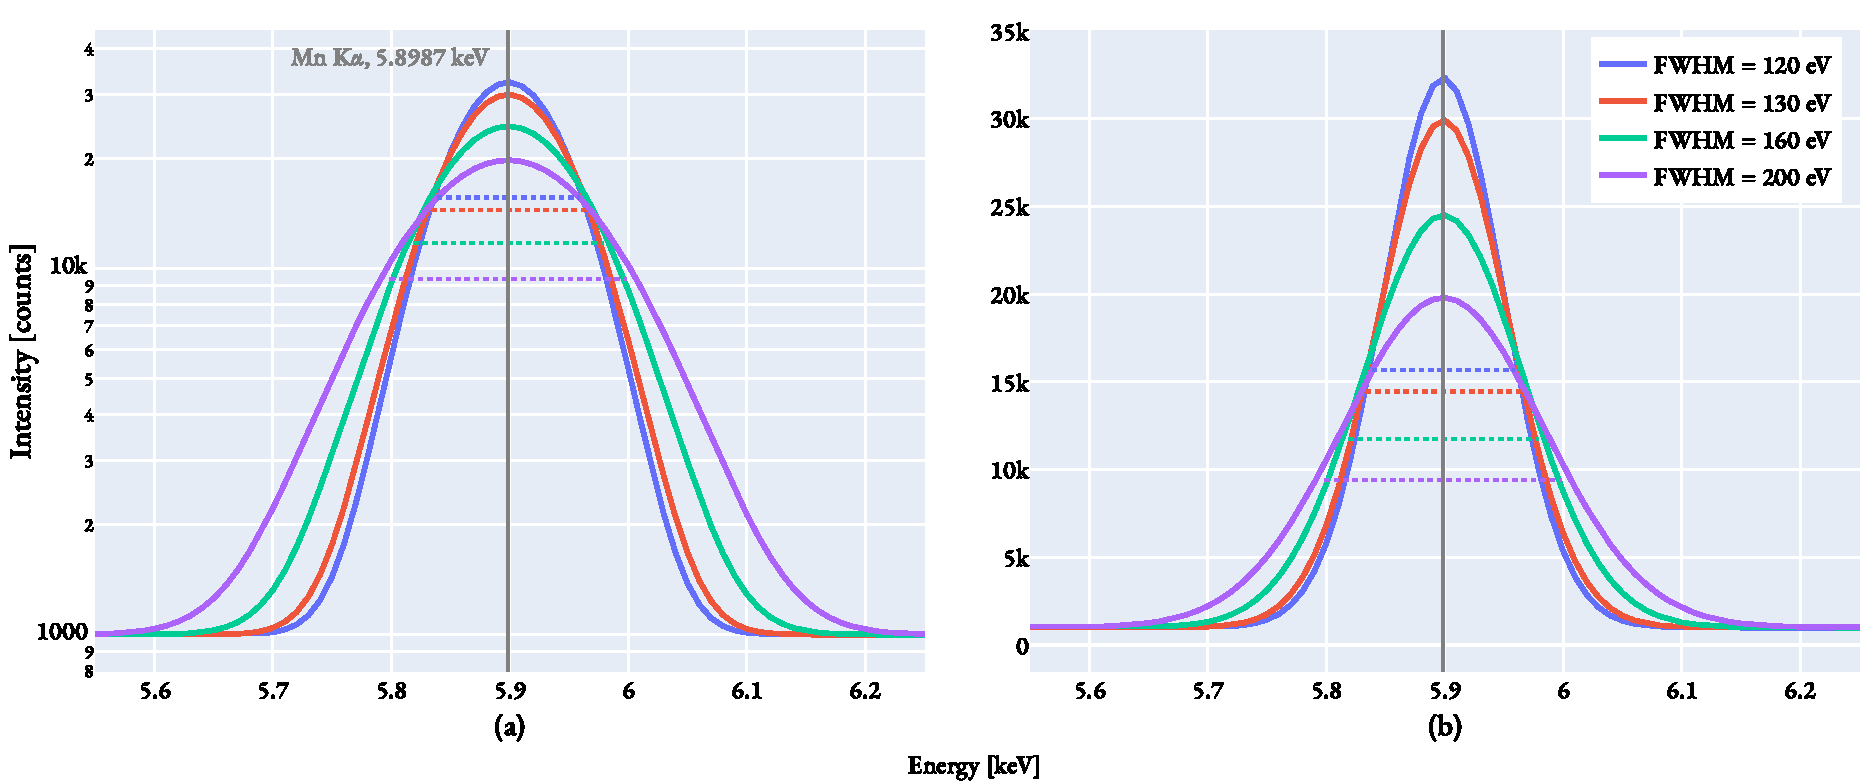
\includegraphics[width=0.95\linewidth]{figures/eds_energyResolutionsMnKa.pdf}
    \caption{
        Illustration of different energy resolutions of EDS detectors.
        The natural line width of the Mn K$\alpha$ line is around 10 eV, but the peak width is more than ten times larger.
        The energy resolution depends on the detector, but also the acquisition parameters.
        The total counts in the peaks are the same.
        The dashed lines are the FWHM of the peaks.
        Panel (a) is a logarithmic y-axis, and panel (b) is a linear y-axis.
    }
    \label{fig:theory:energy_resolution}
\end{figure}





As the electronics broadens the peaks to Gaussian curves, the model fitting of the peaks are done by:

\begin{equation}
    \label{eq:gaussian}
    f(x) = \frac{A}{\sqrt{2\pi}\sigma}\exp\left[{-\frac{(x-x_0)^2}{2\sigma^2}}\right]
\end{equation}

where $A$ is the amplitude, $x_0$ is the mean, $\sigma$ is the standard deviation, and $x$ is the energy.
The model fitting in this thesis is done using the HyperSpy package \cite{hyperspy_1.7.1}.
With the sigma of a Gaussian curve, the full width at half maximum (FWHM) can be calculated as FWHM $= 2\sqrt{2\ln(2)}\sigma$.
% As previously mentioned, 
The detector broadens the peaks, and as different detectors and detector settings can give different peak widths, the FWHM are used as a measurement of the resolution of the detector.


\brynjar{TODO Comment from Ton: "I think here you can also include relation peak width and energy, you have the formula and will use it later to calculate peak width Mn-K from other measured lines."}


\begin{table}[pht]
    \begin{center}
        \caption{
            Definitions for various terms related to EDS detectors, \cref{theory:eds:hardware}. 
            In the order they appear in the text.
            }
        \renewcommand*{\arraystretch}{1.4}
        \label{tab:eds:hardware}
        \begin{tabular}{p{2.6cm}p{12cm}}
            \hline
            \textbf{Name}                   & \textbf{Definition}                                                                                                                                                                                                                                 \\
            \hline
            SDD                             & Silicon drift detector, the most common detector.  High count rates, fast processing, and low capacitance.  See \cref{fig:eds_sdd}.                                                                                                                 \\
            Si(Li) detector                 & The older type of detectors. Much of the literature published is on these detectors.                                                                                                                                                                \\
            Channel                         & A discrete energy interval in the measured histogram. Usually 10 eV.                                                                                                                                                                                \\
            Scale                           & Energy per channel.                                                                                                                                                                                                                                 \\
            Signal intensity                & The number of counts stored in a channel. Signal intensity can also be expressed as counts per second, but counts is used in this work.                                                                                                             \\
            Active layer                    & The part of the detector where the detectable electron-hole pairs are generated.                                                                                                                                                                    \\
            Dead layer                      & The Si layer in the detector where generated electron-hole pair are not drifted to the anode and thus not detected.                                                                                                                                 \\
            Collimator                      & An aperture for the EDS detector, blocking the X-rays with a too high angle, i.e. coming from areas outside the probed spot.                                                                                                                        \\
            Detector window                 & A barrier to keep vacuum in the EDS detector.                                                                                                                                                                                                       \\
            Detector efficiency, $\epsilon$ & The ratio of the detected X-rays to the number of X-rays incident on the active detector are. Some X-rays pass straight through the thin SDD detectors withouth being detected. See \cref{fig:detector_efficiency}                                  \\
            Solid angle, $\Omega$           & The area of the detector that is exposed to the sample. Bigger solid angle gives more counts. $\Omega = \frac{A}{r^2}$, where A is the area of the active layer and r is the distance from the sample to the detector. See \cref{fig:eds_geometry}. \\
            Take-off angle                  & The angle between the sample surface and the detector. TOA increase or decrease with specimen tilt, see \cref{fig:eds_geometry}.                                                                                                                    \\
            Azimuthal angle                 & The angle around the beam (seen from above) between the detector and a reference line, e.g. the chamber door.  See \cref{fig:eds_geometry}.                                                                                                         \\
            Working distance                & The distance between the SEM column and the sample surface. See \cref{fig:eds_geometry}.                                                                                                                                                            \\
            Peak broadening                 & The broadening due to the counting electronics.                                                                                                                                                                                                     \\
            \hline
        \end{tabular}
    \end{center}
\end{table}




























\clearpage



\subsection{The user controlled parameters}
\label{theory:eds:user_controlled_parameters}

The acquisition of EDS spectra is controlled by a set of parameters, which the user can adjust to optimize the analysis.
This section will discuss the most important parameters, and how they affect the analysis.
At the end of the section the parameters are summarized in \cref{tab:eds:userparameters}.

% beam energy
The \textbf{beam energy} ($E_0$) is the kinetic energy of the electrons which are exciting the X-rays, and this energy is set by the acceleration voltage of the electron beam.
The beam energy must be higher than the \textbf{critical ionization energy} ($E_C$) of the element of interest, which is the minimum energy needed to remove an electron from an atom.
The ratio of the beam energy to the critical ionization energy is the \textbf{overvoltage} (U):

\begin{equation}
    U = \frac{E_0}{E_C}
\end{equation}

The overvoltage is different for all the lines in the spectrum, as it is dependent on the critical ionization energy of each line.
When the overvoltage for a specimen is discussed, it is referring to the overvoltage for the line of interest with the highest critical ionization energy.
% Overvoltage is discussed more


% overvoltage and ionization cross-section
To produce a satisfactory amount of X-rays, it is not enough to just have the overvoltage slightly above 1, as the \textbf{ionization cross-section}, $\sigma_T$, plays a critical role.
The ionization cross-section is the probability of an ionization, as described in \cref{theory:xray_formation:intensity} and \cref{eq:ionizationcrosssection}.
The relation between the overvoltage and the ionization cross-section is shown in \cref{fig:overvoltage2ionizationcrosssection}.
% Mari adapted her figure from:
% FIGURE 4.4 - C. B. Carter and D. B. Williams, Transmission electron microscopy: Diffraction, imaging, and spectrometry. Springer, 2009.
As seen in the figure, the probability of ionization increase sharply until U is around 4, and then it decreases.
An equation for the relation between the ionization cross-section and the overvoltage is given in the PAP model for quantitative EDS analysis, which is discussed in \cref{theory:quantitative:pap:general_principle} with \cref{eq:theory:quantitative:pap:calculation_of_F:ionizationcrosssection}, and illustrated in \cref{fig:PAP:ionization_cross_section}.
Having an overvoltage below 1 results in no X-rays generated for the line of interest, which is shown by the line starting at 1.
With SEM EDS the overvoltage is typically in the area where the ionization cross-section is changing the most, thus the overvoltage is an important parameter.
In addition to the effect of the ionization cross-section, the overvoltage is important for how deep the electron can penetrate and still ionize the higher energy lines.
In each scattering process, illustrated in \cref{fig:montecarlo_BSE}, the electron loose energy.
If the overvoltage for a line is 1, an electron which already have scattered and lost some energy will not have enough energy to ionize the line of interest.
This results in fewer generations of X-rays from that line, i.e. low intensity of the line.
As the overvoltage increase from 1, there is an increase in both the ionization cross-section and the amount of electrons with enough energy to scatter multiple times and still ionize the line of interest.
% If the overvoltage for an excitation is 1, the incident electrons can only ionize this excitation close to the surface and will not produce many X-rays.
When the overvoltage is higher, the electrons can scatter multiple times within the specimen before they ionize the highest excitation, which makes the probability of that ionization higher.
ISO 22309 about quantitative analysis in SEM advise an overvoltage of 1.8 \cite{iso_emsa_22029}, and ASTM E1508 on the same topic advise an overvoltage of at least 1.5 \cite{astm_e1508_eds_quantification}.
In Goldstein the advice is to keep the overvoltage above 1.5 \cite[Ch. 20.2.2]{goldstein_scanning_2018}.
A higher overvoltage will produce more X-rays, but also decrease the spatial resolution of the analysis as the interaction volume is increased with $E_0$. % ton: fine section


% figres/overvoltage2ionizationcrosssection.pdf
\begin{figure}[hbt]
    \centering
    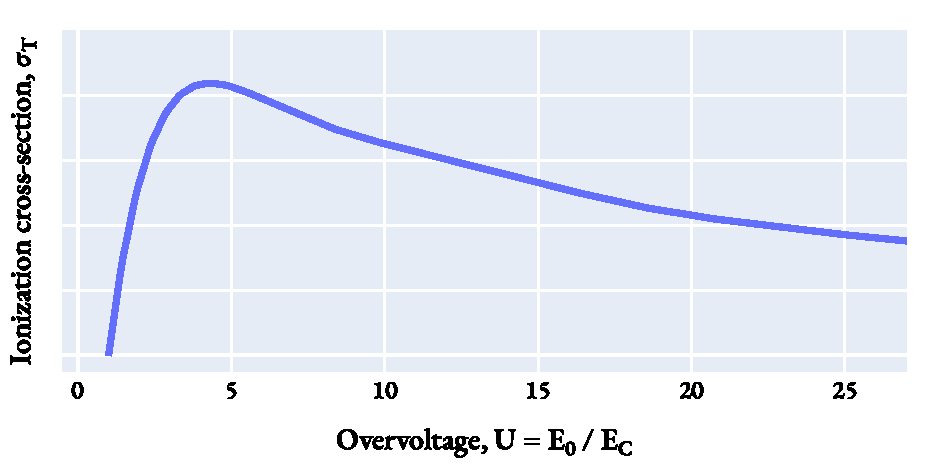
\includegraphics[width=0.6\linewidth]{figures/overvoltage2ionizationcrosssection.pdf}
    \caption{
        The ionization cross-section as a function of overvoltage.
        % The units of $\sigma_T$ are arbitrary
        Adapted from \cite[Fig. 4.4]{williams_carter_tem_2009}.
    }
    \label{fig:overvoltage2ionizationcrosssection}
\end{figure}








% beam current
The \textbf{beam current} ($i_b$) is the current of the electron beam, and is measured in nA or pA.
A higher current will produce more X-rays.
Multiple papers and textbooks like Goldstein advise the measurement of the current hitting the specimen.
This would allow more possibilities for specimen analysis and set-up characterization, for example computing absolute concentrations and calculating the solid angle of the detector.
The beam current is estimated by software, but the current hitting the specimen needs to be measured and this requires addition equipment in the form of a Faraday cup and a good ammeter.
These extra equipment were not available in the present study, but could be a good addition to future work.
The beam current in this work is thus the current set on the SEM and not the current hitting the specimen.
When the current hitting the specimen is discussed, it is referred to as the \textbf{probe current}.
Increasing the beam current do increase the probe current, but some electrons are lost in the SEM column, and the probe current is thus lower than the beam current.
The user can control the beam current directly, but not the probe current.
Some samples are sensitive to beam damage, and on such specimen the beam current should be low.
Controlling the beam current is done to achieve suitable counts per second, depending on what the specimen can cope with without damage and the targeted accuracy of the EDS analysis.


% count rate, ICR and OCR. mention coincidence peaks
The \textbf{count rate} is the number of counts per second (cps), and is affected by multiple factors like the beam energy (probability of X-ray creation), beam current (proportional to creation), the solid angle (detector geometry) and the processing capabilities of the electronics.
A good spectrum needs many counts in total, especially if minor elements in specimens are to be detected and even more when these need to be quantified.
% \brynjar{Is minor and trace elements defined earlier?} % TODO
The number of X-rays per second which produce electron-hole pairs in the active layer of the detector is called the \textbf{input count rate} (ICR).
The number of counts being outputted from the electronics to the memory of the computer is called the \textbf{output count rate} (OCR).
The OCR is limited by the processing capabilities of the electronics, as the electronics needs a certain amount of time to convert the voltage signal into a count.
When a voltage signal is converted into a count, the input of the electronics is shut down for a short time, and this time is called the \textbf{dead time}.
Thus, the OCR is lower than the ICR.
The OCR also include the coincidence peaks, which is when two X-rays are counted as one.
Coincidence peaks are discussed in \cref{theory:eds:artifacts}.
The OCR is the \textbf{throughput} of the detector.
Throughput is a general term for the measure of how much information a system can process per units of time, and in EDS the information is the X-ray counts.



% dead time, live time, and real time
As mentioned above and in \cref{theory:eds:hardware}, the detector needs to shut down the input of the electronics while converting a voltage signal into a count.
This time is called the \textbf{dead time} (DT), and is according to the ISO standard 15632 measured in seconds \cite{iso_qc_15632}.
The dead time is often reported as a percentage of the \textbf{real time}, which is the total time it takes to acquire a spectrum.
The time when the detector is actively detecting X-rays is called the \textbf{live time}, and is the real time minus the dead time.
The dead time can be described by the real time and live time, or by the ICR and OCR.

\begin{equation}
    \label{eq:dead_time}
    % DT = (real time - live time) / real time = 1 - (OCR / ICR)
    DT \% = \frac{\textnormal{Real time} - \textnormal{Live time}}{\textnormal{Real time}} = 1 - \frac{\textnormal{OCR}}{\textnormal{ICR}}
\end{equation}

A high dead time reduce the OCR relative to the ICR.
A higher count rate increase the dead time, as there will be more events to process.
More events per unit of time also increase the probability of coincidence peaks.
Different sources advise slightly different thresholds for the dead time to prevent coincidence peak events.
According to the ASTM 1508 the highest throughput is achieved with a dead time around 40\% \cite{astm_e1508_eds_quantification}.
However, the standard also state that coincidence peak events are beginning to become a problem at dead times above 40\%, and advise dead times between 20\% and 30\% to get good spectra.
Another source, a paper from 2015 by D. Newbury and N. Ritchie on high accuracy quantification with SDDs, advise a dead time below 15\%, preferably below 10\% \cite{newbury_deadtime_2014}.
In Goldstein, it is stated that the Si(Li) detectors handles coincidence events (see \cref{theory:eds:artifacts}) better than SDDs, and that 30\% dead time was "close to optimal for all vendors and most samples" for Si(Li) detectors \cite[p. 466]{goldstein_scanning_2018}.
Further it is stated in Goldstein that SDDs should not be operated according to specific dead times, but rather according to an acceptable low coincidence rate.
With different advice on maximum DT, the best procedure is probably to follow the last advice mentioned from Goldstein.
% This requires the user to make a pre-analysis of the spectrum to determine the coincidence rate, and then adjust the dead time accordingly.
This requires the user to make a pre-analysis of the coincidence rate.


% process time
% Goldstein p 312:
% A short time constant enables more photons to be processed per unit of real (clock) time, but the trade-off of faster processing is poorer accuracy in assigning the photon energy.
The DT is influenced by the \textbf{process time}, which is the time the electronics have to process the signal from the detector.
A longer process time makes the energy resolution better, as the electronics have more time to assess the photon energy.
However, a longer process time also reduce the count rate, as the detector is shut down for a longer time.
Thus, the process time is a trade-off between throughput and energy resolution.


% dwell time, for maps
When mapping a specimen, the \textbf{dwell time} is the time the electron beam is on each position (pixel) the specimen.
Higher dwell time tends to give higher signal intensities and better spatial resolution, but factors like charging, specimen drift, beam damage, and contamination can limit the effect of increased dwell time.
Charging is when the specimen is charged by the electron beam, and can cause the incoming electrons to be deflected.
Charging can be identified by a significant lower effective beam energy than the set beam energy, which is explained in \cref{theory:eds_performance:duanehunt}.
If the specimen is drifting (moving) slightly during the mapping, the spatial resolution will be reduced harshly.
Faster mapping will reduce the effect of specimen drift.
Beam damage on the specimen can change in the chemistry of the specimen or do milling of the specimen surface.
Contamination introduced by the electron beam is typically in the form of carbon, which if present in the chamber can be deposited on the specimen surface by the beam.
Carbon contamination can be revealed by a low voltage SEM image, where the carbon will appear as a darker square on the surface.




%tables/table_eds_userparameters.tex
\begin{table}[pht]
    \begin{center}
        \caption{
            Definitions for various terms related to the user settings in EDS, \cref{theory:eds:user_controlled_parameters}.
            % In the order they appear in the text.
        }
        \renewcommand*{\arraystretch}{1.4}
        \label{tab:eds:userparameters}
        \begin{tabular}{p{2.6cm}p{12cm}}
            \hline
            \textbf{Name}                     & \textbf{Definition}                                                                                                                                                                                                        \\
            \hline
            Beam energy, E$_0$                & The energy of the electrons from the beam when they enter the specimen.                                                                                                                                                    \\
            Critical ionization energy, E$_C$ & The energy required to ionize the element of interest. Dependent on Z and the orbital to excite.                                                                                                                           \\
            Overvoltage, U                    & $ U = E_0 / E_C $, and is required to be at least 1.5 to achieve a good signal from the wanted line.                                                                                                                       \\
            Beam current, I$_0$               & The current used to emit the electrons from the electron gun.                                                                                                                                                              \\
            Probe current                     & The current that hits the specimen.                                                                                                                                                                                        \\
            Count rate                        & The number of X-ray counts per second (cps).                                                                                                                                                                               \\
            Input count rate, ICR             & The number X-rays per second creating electron-hole paris in the active layer in the detector.                                                                                                                             \\
            Output count rate, OCR            & The actual number of counts registered and outputted to the memory. The OCR is lower than the ICR because of the dead time, and because the OCR includes coincidence events.                                               \\
            Throughput                        & How much information a system can process per units of time. In EDS the throughput is the OCR.                                                                                                                             \\
            Real time                         & The time in seconds in takes to acquire a spectrum. Real time = dead time + live time                                                                                                                                      \\
            Dead time                         & The amount of time when the input to the electronics is shut off, because an analouge voltage signals is being converted to a digital count. Dead time is both expressed in seconds and as a percentage of the real time.  \\
            Live time                         & The time in seconds when the detector is actively registering counts.                                                                                                                                                      \\
            Process time                      & A system setting for how much time the electronics have to convert the voltage signal. Longer times give more accurate assessment of the energy. The process time is a trade-off between throughput and energy resolution. \\
            Dwell time                        & The time the electron beam is on each pixel in the 2D image. Higher times increase signal intensities and spatial resolution, but can introduce issues.                                                                    \\
            \hline
        \end{tabular}
    \end{center}
\end{table}

\clearpage


\subsection{Spectral artifacts}
\label{theory:eds:artifacts}



The full spectrum contains the peaks from the characteristic X-rays, the background radiation, and other artifacts.
As the characteristic X-rays and the background have been covered above, this section is an overview of the other artifacts.
These include coincidence peaks, the noise/zero peak, strays/spurious X-rays, the Si escape peak, and internal Si fluorescence peak.
The artifacts can be used to characterize the performance of the detector and the selected settings for the acquisition.
In general, the artifacts are unwanted, as they reduce the signal in the actual peaks and clutter the analysis.
Thus, awareness of the possible artifacts is important for a thorough analysis of the spectrum.
The artifacts are illustrated in \cref{fig:eds_artifacts}, and summarized in \cref{tab:eds_artifacts}.


% Sum peaks
% TODO: only use coincidence, or use the mix?
Acquiring a good spectrum requires a certain amount of counts, but having a high count rate increase the probability of \textbf{coincidence peaks}.
Coincidence peaks are also called sum peaks.
Coincidence peaks are when two X-rays are counted as one, where the assigned energy is the sum of the two X-rays.
If the detector is open and two X-rays hit the active area in the same time window, both X-rays produce electron-hole pairs and the resulting voltage pulse is equal to the sum of the energies.
This effect is called pulse pile-up.
The probability of pulse pile-up is proportional to the count rate.
Different detectors can achieve different count rates, their electronics are designed to handle their possible count rates.
This is reflected in the detectors process time settings, which have to be different for a detector that can reach 1E4 cps compared to a detector that can reach 1E6 cps.
Additionally, the SDD detectors have lower capacitance than the Si(Li) detectors, which makes pulse pile-up problems lower in the SDDs as the electronics can process the pulses faster \cite{astm_e1508_eds_quantification}.
The count rate is related to the dead time through the ICR and OCR, as described in \cref{eq:dead_time}.
As such, it has been common to suggest a certain dead time to avoid coincidence peaks, which is discussed in \cref{theory:eds:user_controlled_parameters}.
A coincidence peak from Si is shown in \cref{fig:background_absorptionEdgeSi}, and coincidence counts from the background is shown in \cref{fig:duanehunt}.
Limiting the coincidence peaks is important for accurate quantification, as the coincidence peaks are counts belonging to other peaks, and a coincidence peak can lead to misidentification of elements not present.

% Coincidence peaks, ASTM 1508:
% "8.3.1 [...] Systems with SDDs generally have smaller pileup
% peaks under the same conditions, because the reduced capacitance
% of the SDD makes it easier for the pulse processing
% electronics to recognize close coincidences as separate events.
% EDS systems often have software to model pileup peaks and
% correct for them."



% Strays
% - Outside the targeted area
% - Si 
% - Holder / chamber 

Another artifact which give similar issues as coincidence peaks is \textbf{stray radiation, or spurious X-rays}.
Strays are X-ray signals which originate from outside the targeted area, and are thus not part of the spectrum of interest.
The strays can be generated from either a deflected electron or from an X-ray through fluorescence.
Deflected electrons are from the beam, or BSE electrons, which both have a high energy.
The fluorescence X-ray are generated by characteristic X-rays or background X-rays, which typically have lower energy than the deflected electrons.
This difference in energy can be used to determine the origin of the strays, which is discussed in \cref{theory:eds_performance:peakratio}, based on the work by Egerton and Cheng \cite{egerton_nio_characterization_1994}.
The spatial regions where a stray X-ray can originate is: (a) inside the specimen, but outside the targeted area, (b) from the chamber, (c) from an eventual specimen holder, and (d) from the detector.
To limit the strays, the collimator in front of the detector is a physical barrier which only allows X-rays from a certain angle to reach the detector.
This requires the detector to be aligned correctly, which could be tested with a tilt series, where the stray signal should be independent of the tilt angle.
The stray signal is made by a combination of the detector and the specimen, thus it is not possible to measure the stray signal in a blank specimen (of vacuum) and subtract that signal from a measurement.
Stray signals need to be handled from case to case, as different specimen give different stray signals on the same detector.
% \ton{Do you want an illustration here of a, b, c, d?} % Answer: No


Strays originating from the (d) the detector results in both the \textbf{internal fluorescence} peak and \textbf{silicon escape peaks}.
The incoming X-ray can ionize Si atoms in the detector.
If the ionized Si is in the dead layer of the detector, the ionized Si will emit a characteristic X-ray which can be detected in the active area of the detector.
This is the internal fluorescence peak, and is located at 1.74 keV, i.e. the Si K$\alpha$ peak.
As SDDs have much thinner dead layers than the Si(Li) detectors, the internal fluorescence peak is much smaller for the SDDs.
The incoming X-ray which ionizes an Si atom loose some energy, which results in the count being recorded at 1.74 keV lower than where the incoming X-ray was supposed to be.
The counts at 1.74 keV lower than the incoming X-ray make the escape peak.
Both escape peaks and sum peaks are most prominent in the strongest line, as there are more events where these artifacts can occur \cite{astm_e1508_eds_quantification}.


% When looking at artifacts from the strongest line, ASTM 1508:
% "9.2.4 While working with the most intense line, look for
% escape and sum peaks. If they are not found for this line, they
% are unlikely to cause interferences. If they are present, keep
% looking for them after other identifications."

% Silicon escape peak, ASTM 1508:
% "8.3.2 A silicon escape peak [...].
% This artifact is greatest at about 2 keV. [...]
% The artifact cannot occur at energies
% below the absorption edge of the Si K line, and it becomes
% negligible at higher energies such as the Cu Ka line. [...]
% SDD are thinner and have more silicon escape peaks."



% Noise peak
Most spectrums have a \textbf{noise peak} around 0 keV, which is present due to electronic noise in the detector \cite{aztec_manual}.
The noise peak is also called the zero peak.
All detectors have this type of noise, but some vendor software remove the noise peak automatically.
The AZtec software does not remove the noise peak, and it is therefore important to be aware of the noise peak.
For example, during model fitting, the noise peak should be removed to avoid a bad background fit in the lower energy region.
The simple solution is to inspect where the noise peak ends, and cut of the spectrum at that energy.
As the noise peak is located sufficiently close to zero, no information is lost by cutting off the spectrum at the noise peak.



% vendor software handling of artifacts
The artifacts mentioned above are in varying degrees present when acquiring a spectrum, but some vendor software have built-in methods to remove or reduce the artifacts.
In Goldstein at page 274, it is shown that an escape peak was present using the 2011 software, but automatically and digitally removed in the 2014 software \cite[Fig. 18.7]{goldstein_scanning_2018}.
The AZtec software have a built-in method to remove coincidence peaks, called "Pulse Pile Up Correction" \cite{aztec_manual}.
The AZtec user manual state that this method works best for single pixels or areas with the same composition, and that it might produce bad results when scanning over a larger heterogeneous area \cite[p. 99]{aztec_manual}.
Aside from this brief description, a user does not get any information on how the method works.
This illustrates one of the challenges with digital solutions implemented by the vendors, as the software is a black box which can enhance the spectrum, but also produce bad results due to incorrect handling of artifacts. %can produce bad results.


% figures/artifacts.pdf
\begin{figure}[htbp]
    \centering
    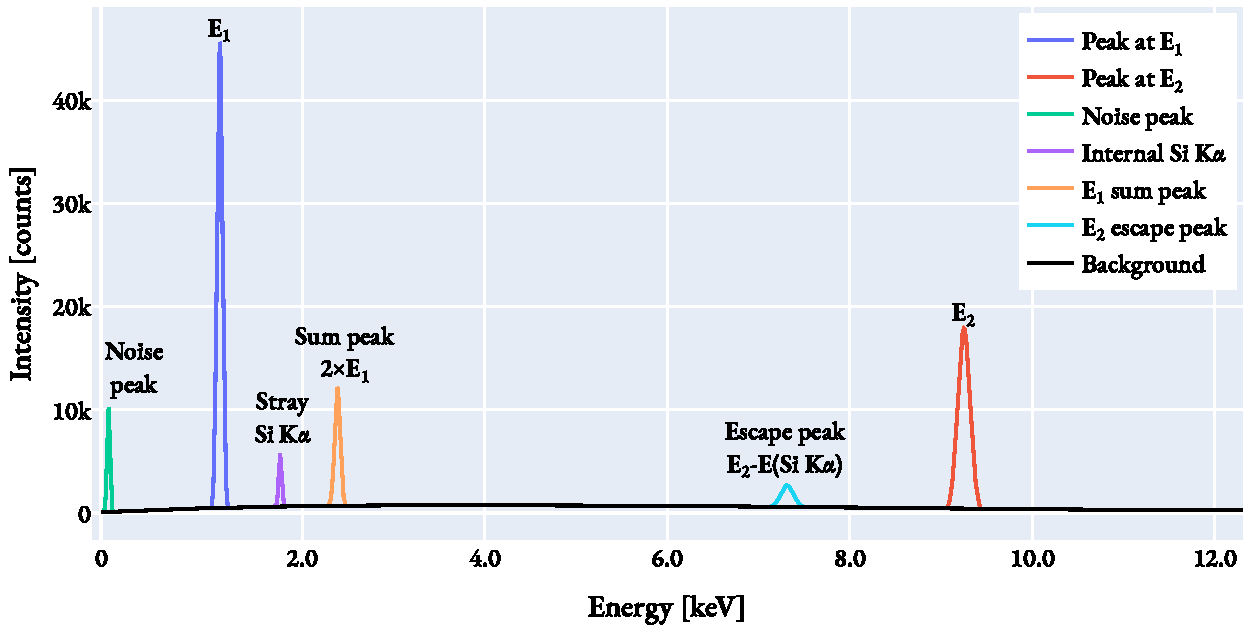
\includegraphics[width=0.95\linewidth]{figures/eds_artifacts.pdf}
    \caption{
        Some of the possible artifacts in EDS spectra.
        Ton: "Is noise peak that high? Should it be on 0 eV as stated in text?"
        Brynjar: "Her er det noe rart med x-aksen, og kan gjøre noise peak lavere."
        \brynjar{TODO: redo this figure.}
    }
    \label{fig:eds_artifacts}
\end{figure}


\begin{table}[hbtp]
    \begin{center}
        \caption{
            The spectrum artifacts in EDS, \cref{theory:eds:artifacts}.
            See \cref{fig:eds_artifacts} for an illustration of the artifacts.
        }
        \renewcommand*{\arraystretch}{1.4}
        \label{tab:eds_artifacts}
        \begin{tabular}{p{4cm}p{10.6cm}}
            \hline
            \textbf{Artifact name}     & \textbf{Definition}                                                                                                                                                                                                                   \\
            \hline
            Background X-rays          & The white noise generated as $1/E_0$. The detected background is reduced at low energies due to absorption, see \cref{fig:background_xrays}.                                                                                          \\
            Coincidence peaks          & When two X-rays are counted as one, resulting a count at the sum of the energies. Increase with count rate, but advices to limit the artifact is usually given in terms of dead time. See \cref{fig:background_absorptionEdgeSi}. \\
            Stray radiation            & X-ray signals which originate from outside the targeted area. Generated from deflected electrons or X-ray photons. Can originate from the specimen, the chamber, an eventual holder, or the detector.                                 \\
            Internal fluorescence peak & A stray from the detector at $1.74$ keV, due to ionization of Si in the detector, which emits a Si K$\alpha$ X-ray that afterwards is registered by the detector.                                                                       \\
            Escape peak                & A signal from a characteristic line which have lost $1.74$ keV due to its ionization of an Si atom in the detector.                                                                                                                     \\
            Noise peak                 & The peak around $0$ keV, which is present in all detectors due to electronic noise.                                                                                                                                                     \\
            % Software correction        & Some vendors have software which reduce or remove the artifacts in the spectrum.                                                                                                                             \\
            \hline
        \end{tabular}
    \end{center}
\end{table}


\clearpage








































\section{EDS performance parameters}
\label{theory:eds_performance}

% TON: wants this to be "EDS characteristic parameters" or something like that


% For detection characteristics you list , the details and references are OK, but again guide the reader, certainly as the list is long and details are specific. Per item define clearly what it is, give first the definition before discussing it. I am considering if a schematic spectrum can help where you point to aspects that matter help. Motivate and introduce schematically , in a sub section called, overview/Schematic representation, before going into details. Some are set-up, some are geometry, some are electronic hardware related. At end or in experimental chapter and again in discussion, can summarize all in a table with references to literature and the section where quantities are introduces. This is core of your work, has an added value for reader (not common knowledge)and therefore can be longer. 

The aim of this work is to improve EDS bulk quantification, and one way to do that is to improve the performance of the EDS setup, which is the upper row in \cref{fig:intro:parameters}.
Identifying potential issues with the EDS setup can be done through certain performance parameters.
A performance check can reveal errors in the setup and acquisition parameters, and it can make the input parameters for the quantification more accurate.
Vendors of EDS detectors like Oxford Instruments provide a guide for how to calibrate their detectors, but these guides are limited to calibration of energy resolution and scale \cite{aztec_manual}.
As both Thompson in \cite{keith_energy_res_2013} and Goldstein in \cite{goldstein_scanning_2018} writes, the state of an EDS setup is characterized by more than its energy resolution and scale.
In 1986 Williams criticized the lack of standardized performance criteria for EDS in AEMs \brynjar{TODO: define AEM earlier?}, and suggested three standardized metrics \cite{williams_standard_definitions_1986}, but these metrics were not widely adopted.
Routines for a performance check seems to vary significantly between different laboratories, and the industry and standard authorities have not yet agreed on a standard set of metrics, aside from the energy resolution, measured by the FWHM the Mn K$\alpha$ line.


% not new paragraph?
An ISO standard for selected SEM EDS performance was introduced in 2002 (revised in 2012 and 2021), which includes details on calibration metrics \cite{iso_qc_15632}.
% \brynjar{This standard was discovered late february 2023. However, a Jupyter notebook is stil relevant to show how to do the calculations, and this thesis explain the relevance of the metrics.}
Some literature is available on performance parameters for TEM EDS setups, e.g. the work of Egerton and Cheng \cite{egerton_nio_characterization_1994}, updated and easily accessible in the info-sheet by Ted Pella \cite{ted_pella_nio_tem_2019}, which also sells NiO test standards.
Literature on performance parameters for SEM EDS setups are less common, but some papers \cite{software_dtsaii,dtsaii_1_getting_started,dtsaii_2_manipulating_spectra} are available and the software DTSA-II includes a quality control program, described in the textbook by Goldstein \cite{goldstein_scanning_2018}.
Goldstein also include details on a range of parameters, such as linearity and stability of the detector, along with possible SEM EDS issues, such as beam-sensitive specimen and specimen with irregular topography \cite{goldstein_scanning_2018}.
The similarities between EDS in SEM and TEM allow much overlap in the performance parameters, but there are also some differences.
One of the challenges in this work is to find the most relevant test characteristics for SEM, and especially what ranges of values should be acceptable for a well performing detector.
\brynjar{TODO: Get these ranges/value numbers into results and the discussion, and link back here.}
Out of range values could indicate a suboptimal set-up or affect calculating composition.
Identification of set-up parameters with optimization and correction should lead to better EDS analysis.
The value range challenge is affected by both the change from TEM to SEM and the change from the older Si(Li) detectors to the now more commonly used SDDs.
In this section, each of the test characteristics is described with what it is, how it is measured, and what values are acceptable.
Before the test characteristics are described, an overview is given and a summary table is given at the end of the section in \cref{tab:eds_performance_parameters}.

% Mari: The tests are described by Watanabe in [30] and in the info-sheet by Ted Pella [33] which is based on the original work by R.F. Egerton and C.S. Cheng from 1994 [16].
% The complete test routine has several characteristics. Here only the most essential to this work are discussed, and an overview is found in Tab. 2.3.


\subsection{Overview}
\label{theory:eds_performance:overview}

\brynjar{Rethink order. Ton: "For me the logic order would be, Overview, Scale and offset, energy resolution, deviations positions, Fiori, DH as this order you will do it, importance and reading plot left to right."}

% 35
%   Duane-Hunt limit 
%   Energy resolution 
%   Scale and offset 
%   deviations in peak positions 
%   Fiori peak-to-background ratio 
%   Peak ratios - contamination and stray radiation 
%   XXXXX Peak shape XXXXX
%   Number of counts in peaks vs background 
%   Other tests - stability and linearity 
%    What material to use? 
%    Regarding the ISO 15632 standard 
%    Stuff to add / notes 



The performance parameters presented below are divided into two categories: detector and acquisition parameters.
The detector parameters are related to the detector itself, while the acquisition parameters are related to the acquisition setup.
These performance parameters do not include the data treatment step, illustrated in \cref{fig:intro:parameters}, as it is a characterization of the detector and acquisition setup.
The parameters of the detector are: energy resolution, the energy scale and offset, peak ratios, and deviations in peak positions.
The parameters of the acquisition are: the Duane-Hunt limit, the Fiori peak-to-background ratio, and portion of counts in peaks vs background.
The energy resolution is affected by both the detector and the acquisition setup.
At the end there is a section on other test, which are of interest but have not been included in this work.


% questions that the pp can answer
The goal of the performance check is to identify potential issues with the detector and acquisition setup.
Is the detector performing as expected and stated in the specifications?
Is the spectrum reflecting the acquisition parameters set by the user?
How well are the peaks defined?
Are the peaks in the correct positions?
Can the spectrum reveal contamination?
Is the spectrum affected by stray radiation?
The performance parameters described in this section can be used to answer these questions.
At the end of the section, \cref{tab:eds_performance_parameters} contains a summary of each parameter, and what it can reveal.
% \brynjar{Maybe add some schematics for this intro section.}



% a schematic of the performance parameters
\cref{fig:theory:eds_performance:overview:duanehunt,fig:theory:eds_performance:overview:fiori_snr,fig:theory:eds_performance:overview:peak_deviations,fig:theory:eds_performance:overview:strays} are schematic illustrations of the performance parameters.
\cref{fig:theory:eds_performance:overview:duanehunt} shows the Duane-Hunt limit, which is the minimum beam energy required to produce a signal.
\cref{fig:theory:eds_performance:overview:fiori_snr} shows the different signal-to-noise ratios, which is quantified by the Fiori peak-to-background ratio.
The same illustration shows different background portions.
\cref{fig:theory:eds_performance:overview:peak_deviations} shows the deviations in peak positions, which is an affected by the energy scale and offset, and which part of the spectrum is used for calibration.
\cref{fig:theory:eds_performance:overview:strays} shows the effect of stray radiation, which is can be quantified by calculating peak ratios between a stray and a non-stray peak.
Energy resolution is illustrated above, in \cref{fig:theory:energy_resolution}.

% figures/pp_duane-hunt.pdf

\begin{figure}[htp]
    \centering
    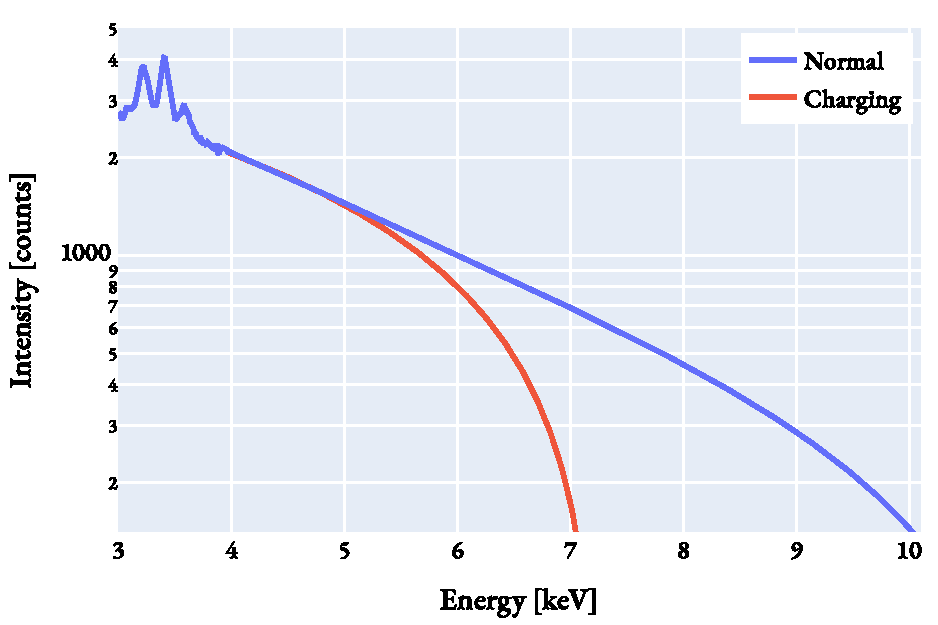
\includegraphics[width=0.6\linewidth]{figures/pp_duane-hunt.pdf}
    \caption{
        Illustration of a spectrum where the Duane-Hunt limit is different due to charging.
        The charging sample (red) has a lower effective beam energy than expected (10 keV).
        The sample with good conductivity (blue) has the expected beam energy (10 keV).
    }
    \label{fig:theory:eds_performance:overview:duanehunt}
\end{figure}


% figures/pp_fiori_snr.pdf
\begin{figure}[htp]
    \centering
    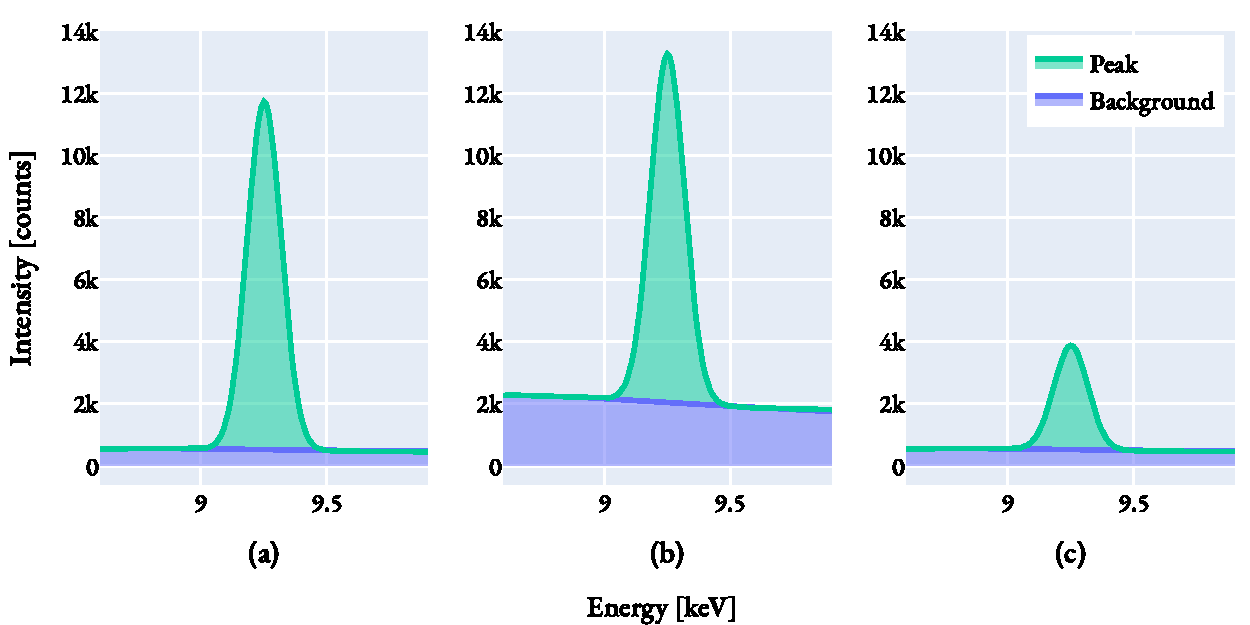
\includegraphics[width=0.8\linewidth]{figures/pp_fiori_snr.pdf}
    \caption{
        Illustration of different spectra with signal-to-noise ratios.
        The peak intensity is the green area, and the background is the blue.
        Panel (a) has a high SNR.
        Panel (b) has a lower SNR due to a higher background intensity.
        Panel (c) has a lower low SNR due to a lower peak intensity.
        Even though this illustrative background is linear, that is not always the case.
        \brynjar{Is background fitting covered somewhere?}
    }
    \label{fig:theory:eds_performance:overview:fiori_snr}
\end{figure}


% figures/pp_peak_deviations.pdf
\begin{figure}[htp]
    \centering
    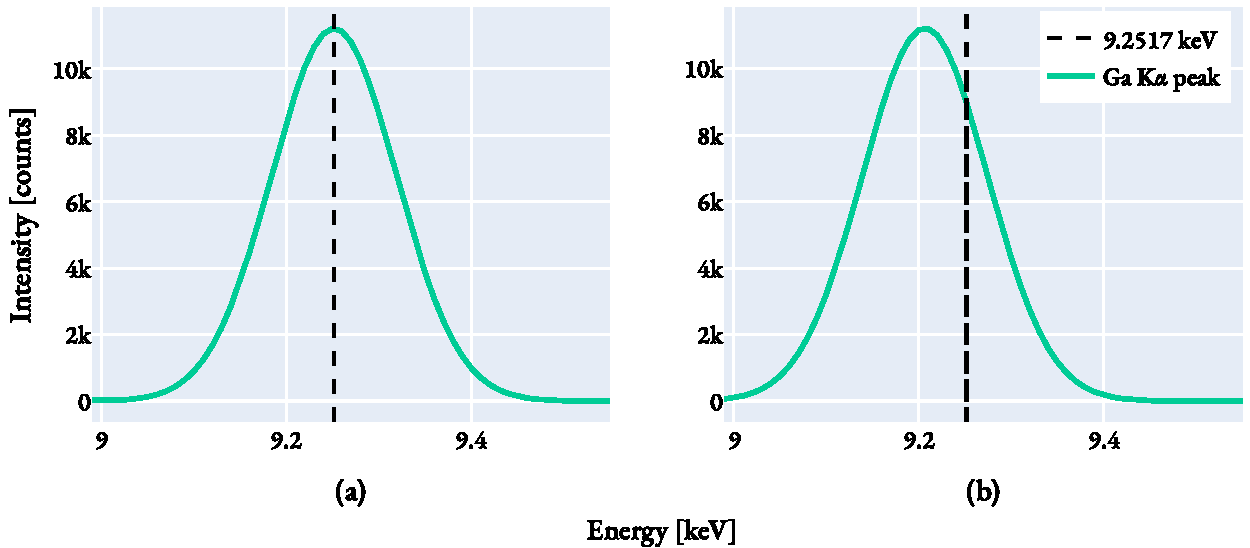
\includegraphics[width=0.8\linewidth]{figures/pp_peak_deviation.pdf}
    \caption{
        Illustration of peak deviations.
        Panel (a) is well calibrated for the medium high energy Ga K$\alpha$ peak.
        Panel (b) is calibrated for low energy peaks, but the Ga K$\alpha$ peak is shifted.
    }
    \label{fig:theory:eds_performance:overview:peak_deviations}
\end{figure}

% figures/pp_strays.pdf
\begin{figure}[htp]
    \centering
    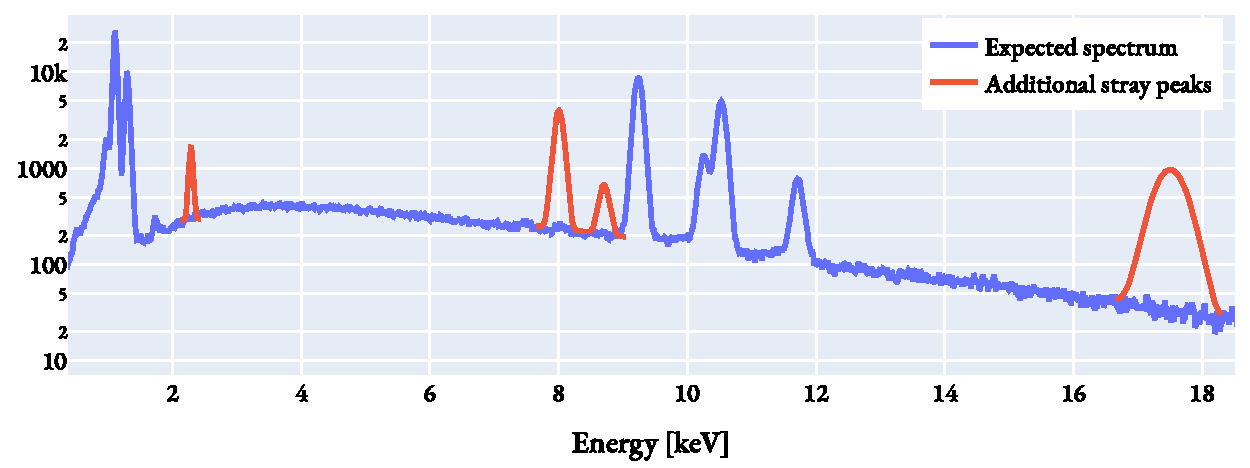
\includegraphics[width=0.8\linewidth]{figures/pp_strays.pdf}
    \caption{
        Illustration of strays.
        The expected spectrum (blue) has additional peaks (green) due to stray radiation.
        The example is a GaAs sample with strays of Mo L$\alpha$, Cu K$\alpha$, Cu K$\beta$, and Mo K$\alpha$.
        \brynjar{Add Mo Kb? And Cu La?}
    }
    \label{fig:theory:eds_performance:overview:strays}
\end{figure}




% what materials to use for the tests
Recording the necessary metrics for the performance parameters requires a sample with some specific properties.
The test sample should be homogenous with a known composition, and the elements present should have lines at both low and high energies.
The lines should not be high enough to cause overvoltage issues, as was noted with Mo K$\alpha$ in \cite{project_report}.
Even at 30 kV, the Mo K$\alpha$ line at 17.47 keV had very low intensity, making the analysis done with this peak less reliable.
The peaks in the spectrum should overlap less than the expected energy resolution and preferably be well separated, as this will make the fitting of the peaks less accurate.
For repeatability, the sample should not be reactive.
Additionally, the sample should preferably both be easy to acquire and not expensive.
When vendors, like Ted Pella who provides the NiO test sample for TEM, are used, the sample might not be available immediately, and the delivery time can be long, as experienced during this work and in the project report \cite{project_report}.

% Low and high lines. Not a overvoltage issue in SEM. Also viable for low energy? Clear peaks, not severe overlap issues.
% Easy to find. Not expensive. Not restricted by delivery from a vendor. Not reactive.






\subsection{Duane-Hunt limit}
\label{theory:eds_performance:duanehunt}
% put after calibration? It is done before in the code, but it is not a part of AZtec.

% What
The Duane-Hunt limit is the maximum energy of the X-ray background radiation, which originates from a paper from Duane and Hunt in 1915 \cite{Duane_Hunt_1915}.
The acceleration voltage selected by the user is the nominal beam energy, while the effective beam energy is the Duane-Hunt limit, and these two values can deviate significantly.
The effective beam energy is the incident beam energy, $E_0$, that excites X-rays in the specimen.
As seen in \cref{fig:duanehunt}, the detected X-rays decline rapidly and linearly towards the nominal beam energy, but the counts does not go to zero.
It is not possible to excite X-rays above the effective beam energy, thus the spectrum should be cut off at the beam energy to allow better model fitting.
The counts above the Duane-Hunt limit are due to coincidence events, where two X-rays are detected as one, as explained in \cref{theory:eds:artifacts}.


% How
Finding the effective beam energy is done by fitting a linear function to background, where the intersection of the linear fit and the x-axis is the effective beam energy \cite{software_dtsaii} \cite[Ch. 9.1.3]{goldstein_scanning_2018}.
This solves the ambiguity of the exact beam energy, which is present because of the coincidence counts that gives the spectrum a tail past the effective beam energy.

% figures/Duane-Hunt.pdf
\begin{figure}[ht]
    \centering
    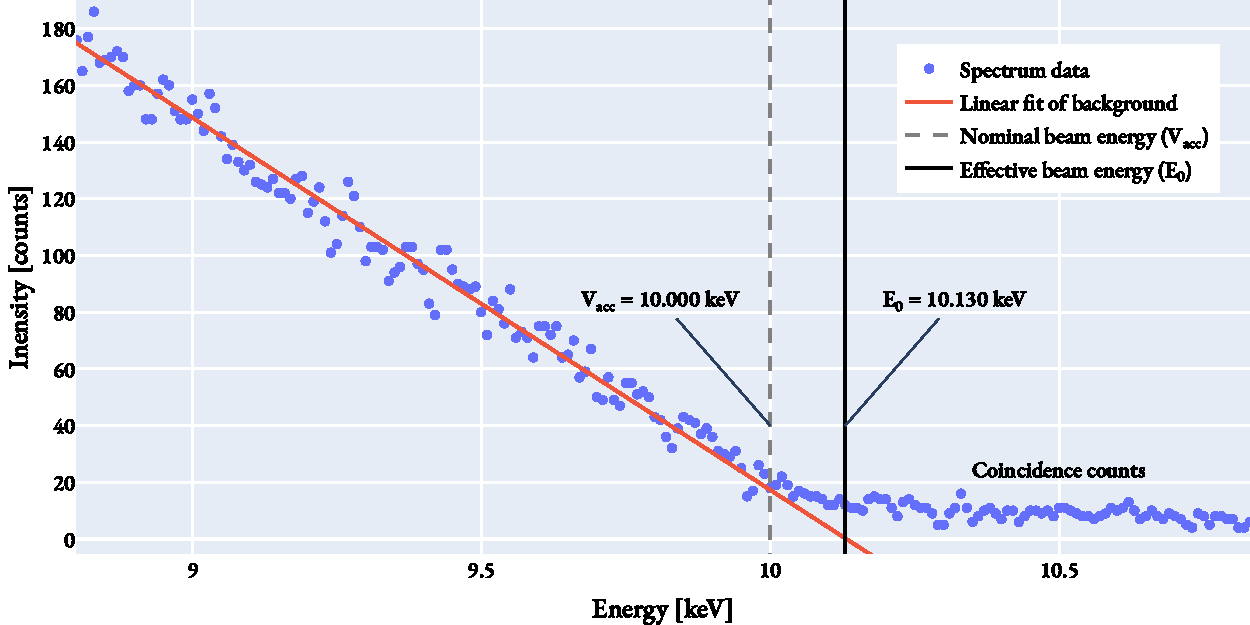
\includegraphics[width=0.8\linewidth]{figures/Duane-Hunt.pdf}
    \caption{
        Illustration of the Duane-Hunt limit.
        The blue dots are the X-ray counts, and the red line is a linear fit of the background.
        The gray dashed line is the nominal beam energy, and the black line is the effective beam energy.
    }
    \label{fig:duanehunt}
\end{figure}


% Acceptable values
There will be some deviation between the nominal beam energy and the effective beam energy, typically up to 0.2 keV.
Different specimen will have different deviation, due to varying conductivity.
Specimen with low conductivity will get problems with charging, which will lowers the effective beam energy.
Thus, a deviation between the nominal and effective beam energy of several kilo-electronvolts is a sign of charging \cite{dtsaii_2_manipulating_spectra}.
Charging of specimen are covered in detail in a paper by Postek and Vladár \cite{postek_charging_2015}.
Another explanation of a large deviation is that the voltage indicated by the SEM is imprecise.
In both cases, a quantitative analysis will yield poor results \cite{iso_emsa_22029}.
Thus, the Duane-Hunt limit relates the acceleration voltage and the conductivity of the specimen.
\brynjar{TODO: discussion, "Is it a useful test for you, for given HT and good conducting specimen? Comment this in discussion?" No, it is not very useful, but nice for slicing.}

% \brynjar{ISO 22309 Quantitative: " 5.6 For standardless analysis, check the measured spectrum using the Duane-Hunt rule.
% NOTE - Deviations of the high-energy end of the bremsstrahlung background from the indicated high voltage means
% either charging of the specimen or a wrong high voltage indicated by the SEM. No quantitative analysis can be done in
% these cases."}

% \brynjar{ASTM 1508: Vacc is not always the same as effective beam energy.
%     "The actual accelerating voltage of the electron beam does not
%     always correspond with the voltage selected on the instrument.
%     It can be determined by expanding the vertical scale of the EDS
%     spectrum and observing the energy above which continuum X
%     rays do not occur."
%     From Ritchies PP: The Duane-Hunt is useful not so much to test the EDS detector as to ensure
%     the accelerating voltage is correct and to demonstrate that there is a
%     conductive path from the stage to ground.}






\subsection{Energy resolution}
\label{theory:eds_performance:energyres}


% What, Mn Ka
The energy resolution of an EDS system is the ability to distinguish two lines at different energies, and is measured by the FWHM of the Mn K$\alpha$ peak.
Two partly overlapping peaks have high contrast if the peak maximums and the valley between the peaks are well separated.
The contrast increase with the energy resolution, as the peaks are more separated.
The convention of using the Mn K$\alpha$ peak as the reference for the energy resolution is because of its position at 5.8987 keV, which gives an indication for both the lower and higher energies used in EDS.
% The sentence below is repeated too much:
% The first SDD detectors had an energy resolution between 160 and 200 eV, while modern detectors can achieve energy resolution around 120-140 eV, which allow closer peaks to be separated \cite{keith_energy_res_2013,goldstein_scanning_2018}. % \brynjar{Thompson refers to Goldstein\dots}.
All EDS detectors have a stated energy resolution in its specifications, however the actual resolution of a given spectrum varies some with the acquisition settings for the same detector.
Thompson shows that with the dead time kept constant, a higher input count rate gives worse resolution, with the example of 121 eV resolution with <5000 cps, and 140-150 eV resolution with >100,000 cps \cite{keith_energy_res_2013}.
Thompson claims that EDS specifications are based on acquisition designs with low input counts.
The process time setting is also affecting the energy resolution.
A longer process time gives the electronics more time to process and assign the energy of the incoming count, and thus gives better resolution.
However, a long process time gives lower count rates and longer acquisition times.
% Dette under må være en glipp
% Changes in dead time are also affecting the energy resolution, where shorter dead time give degraded resolution, because a lower dead time gives the computer shorter time to process the incoming signal and sets the channel value less accurate of each count \brynjar{Ref?}.


% Other FWHMs
Even though the Mn K$\alpha$ peak is the most common reference for the energy resolution, other peaks can be used to get additional information.
Detectors which shall perform at low energies (>1 keV), should also report the FWHM of F, and possibly of C.
This is the advice given in the ISO 15532 standard \cite{iso_qc_15632}.
As this low energy range is not the main focus of this thesis, such low energy peaks have not been included in the specimen used for the tests.
The remainder of this section will focus on the Mn K$\alpha$ peak.


% Approaching the theoretical limit? Find source, Goldstein?
% TODO: amplifier noise is described with an equation in Woldseth 1973, referenced in bennett_egerton_1995.
% Woldseth 1973 figure remake in Goldstein 2003 3rd ed.: It can readily be seen that even if the noise contribution were totally eliminated, the theoretical energy resolution limit would still be greater than 100 eV for Fe Ka at 6.4 keV

% How

Three different approaches to measure the energy resolution are described below.
The first is to directly measure the Mn K$\alpha$ peak in a specimen with Mn.
The second is using the Ni K$\alpha$ peak and multiply it by a factor of 0.926, which is suggested by Ted Pella, Inc. \cite{ted_pella_nio_tem_2019}.
The third is to use any peak in the spectrum, and calculate what the energy resolution would be if there was a Mn K$\alpha$ peak in the spectrum, using \cref{eq:estimateFWHM}.
The second approach is a special case of the third, where the Ni K$\alpha$ peak is used as the reference peak, but with a much simplified equation which is only valid in certain FWHM ranges.
\brynjar{Test litt denne 0.926 faktoren med formelen til metode 3. Eventuelt skriv om forrige setning.}
The third approach is the one which is used in the code developed in this work.


% Direct measurement
% \brynjar{Implement check for Mn K$\alpha$ peak in the code?}
The industry standard for the energy resolution is to measure the FWHM of the Mn K$\alpha$ peak generated by an Fe$^{55}$ source, when the detector is off the microscope.
This is the advised method in the ISO 15632 on EDS performance parameters \cite{iso_qc_15632}.
The argument for doing this is that the energy resolution is not a function of the microscope, thus measuring the energy resolution off the microscope negates all possible influences from the microscope.
The ISO standard recognize that this is not easily done by users, and thus suggesting polished Mn as a substitute.
% The most straight forward way of finding the energy resolution  is to measure the FWHM of the Mn K$\alpha$ peak in a sample with Mn, preferably with high concentration as that provides a well defined peak.
The FWHM measurement should be from a numerical fitting of a Gaussian to the peak, because it limits the effect of the background, and it uses all the information in the peak instead of just three points (the peak maximum, the left and right half maximum).


% Ni Ka * 0.926
Another approach, which can be used when a sample with Ni is available, is to measure the FWHM of Ni K$\alpha$ and multiply the value with 0.926 \cite{bennett_egerton_1995}.
This approach is based on a study in 1995 \cite{bennett_egerton_1995} where five TEM laboratories were given a standard NiO test specimen with a series of EDS test measurements to be done, where one of the tests were focused on the energy resolution.
The test used the Ni K$\alpha$ and O K$\alpha$ peaks, where the FWHM of these two lines were measured, and a linear correlation between photon energy and the square of the energy resolution was assumed.
Then the FWHM of Mn K$\alpha$ was determined by interpolation, and the factor 0.926 was reported as a sufficiently good conversion from Ni K$\alpha$ to Mn K$\alpha$ for the five TEM laboratories.
This approach is the recommended method provided by Ted Pella Inc., who manufactures standardized NiO test specimens for TEM \cite{egerton_nio_characterization_1994,ted_pella_nio_tem_2019}.


% HyperSpy
A third and more general approach, is to use the energy calibration method in HyperSpy, which estimates the FWHM of Mn K$\alpha$.
The method, \verb|EDSModel.calibrate_energy_axis()|, is available for EDS spectrum from SEM and TEM.
The method has two default arguments: \verb|calibrate='resolution'| and \verb|xray_lines='all_alpha'|.
The estimation of the FWHM of Mn K$\alpha$ is done in two steps.
The first step is to fit the width of all the lines in the spectrum, which is needed to get a correct reference peak width, i.e. an account for the peak broadening of the detector.
% \ton{This I read from the HS code, line 50 in: \url{https://github.com/hyperspy/hyperspy/blob/842d6d9713d866960a033d4006200a43841079fe/hyperspy/models/edsmodel.py}}.
The second step utilizes an equation by Fiori and Newbury from a conference paper in 1978, and while this original paper is hard to get hold of (neither the NTNU library or paper depositories could provide it), the equation is included in Goldstein \cite[Ch. 16.1.1]{goldstein_scanning_2018} with a reference to the original paper\footnote{One of the two authors of the original 1978 publication is D. Newbury, who is also the second author of the Goldstein textbook \cite{goldstein_scanning_2018}.}
The equation use one known line in the spectrum to estimate what the FWHM would be at an arbitrary energy:
% \brynjar{original: Fiori, C. E., and Newbury, D. E. (1978). In SEM/1978/I, SEM, Inc., AFM O'Hare, Illinois, p. 401.}

\begin{equation}
    \label{eq:estimateFWHM}
    \textnormal{FWHM}(E) =  \sqrt{2.5 \cdot (E - E_\textnormal{ref}) + \textnormal{FWHM}^2_{\textnormal{ref}}}
\end{equation}

Where $E$ is the energy of the wanted FWHM, i.e. Mn K$\alpha$ for estimating the energy resolution.
$E_\textnormal{ref}$ is the energy of a reference line in the spectrum, and $\textnormal{FWHM}_{\textnormal{ref}}$ is the FWHM of that line.
Both the energies and FWHMs are in eV.
When using the HyperSpy method \verb|calibrate_energy_axis|, the user should be aware of the argument \verb|xray_lines|, which can either be a list of strings with line names or \verb|'all_alpha'|, the latter being the default value for the argument.
As of HyperSpy v1.7.3, the reference line in \cref{eq:estimateFWHM} is the first line in \verb|xray_lines|, which becomes the alphabetically first line when using \verb|'all_alpha'|.
The fact that the reference line is only the first line in the list, is not documented clearly in the HyperSpy documentation, and can yield unexpected results when the first line is not a well-defined peak.
The method works well when the reference line is a well-defined peak.
\brynjar{Should probably give a definition of "well-defined" \dots}
Setting the energy resolution of a spectrum could be done as the average of several distinct peaks, it could be the lowest estimate, the average of the three lowest, or another selection.
For comparative purposes, the same selection should be used, and it should be clear which selection was used.
This is a focus in this work.
\brynjar{Add average, best, and average of three best, and evt some more to the results.}
% TODO \brynjar{Discuss: when taking a series of spectra with different Vacc, the first line (eg AsKa in GaAs or AlKa in SU9000) is poorly defined for 10 kV and 5 kV respectively, resulting in weirdly poor Mn Ka estimate.}



% TODO: bruke average istedenfor én peak? forskjellige peaks gir forskjellige tall
% Er det best om det er user defined peak?


% what the vendors say
As the energy resolution is a function of the count rate and the process time, it is probable that EDS vendors report the energy resolution with a low count rate and a long process time.
To clarify such possibilities, the ISO standard state that the ICR should be < 1000 cps when the best energy resolution is reported \cite{iso_qc_15632}.
Further, the standard states that detectors with possibilities for high count rates should also specify the energy resolution at a high count rate, e.g. 1E6 cps.
This is, to the knowledge of the author, not commonly done by SEM and TEM EDS detector vendors.
% TODO: Add smt about this in discussion

% \ton{OK to use the previous sentence?} Answer: " Ithink it is not practically happen. However, there might be industrial special EDS systems that operate over large count ranges I guess. The comment, you concluding comment is fine, keep as it is."


% Acceptable values
% \ton{This paragraph about acceptable values are bad. Any suggestions here?}
The energy resolution of a taken spectrum should be close to what the specifications of the EDS.
Deviations below the specification should raise suspicion, as energy resolution is one of the main selling points that EDS detector vendors use.
Deviations above the specification should be related to the acquisition settings set by the user.
If the user cannot achieve the energy resolution in the specification with optimal settings, the user should probably contact the EDS detector vendor for support.
In Goldstein, it is stated that most specimen would benefit of a small loss in energy resolution to get higher throughput \cite[16.3.2]{goldstein_scanning_2018}.
The trade-off between energy resolution and throughput allows a small loss in resolution for a high gain in throughput.
However, the user must be aware of the elements in the specimen, as overlapping peaks become more difficult to resolve with a lower energy resolution.
Thus, the user should adjust the trade-off according to the specimen used and the aim of the analysis.

% e.g. deviations when using the HS method implicate that the reference line is not a well-defined peak, which can be caused by ...
% As explained, the theoretical limit of the FWHM of Mn K$\alpha$ is XXX \brynjar{explain above!}.
% The HyperSpy method will raise an ValueError if the estimated energy resolution is below 110 eV \brynjar{line 450, \url{https://github.com/hyperspy/hyperspy/blob/842d6d9713d866960a033d4006200a43841079fe/hyperspy/models/edsmodel.py}}.

% The ISO standard
% \brynjar{ISO 15632: "The
%     resolution value shall be accompanied by a statement of count rate for which the specification is valid.
%     For most detector systems the best energy resolution is attained at an ICR < 1 000 counts/s and the
%     best energy resolution shall be specified. Where detector systems offer higher count rate capability, e.g.
%     SDD EDS, the energy resolution shall also be specified at high ICR, e.g. 50 000 counts/s, 500 000 counts/s."}








\subsection{Scale and offset}
\label{theory:eds_performance:scaleoffset}

% scale and offset in one subsection?

% % What
% What is the scale and offset.
% Typical values for the scale.

The scale and offset are the parameters used to set the energy axis.
The scale is the energy width of one channel, and the offset is the energy of the first channel in the spectrum.
Another name for the scale is the gain or the dispersion.
Calibration of the energy axis is done by: (1) fitting the background and Gaussian curves to the peaks in the spectrum, (2) calculate the theoretical energy difference between two or more peaks, and (3) use the difference between the theoretical and the measured energy difference to calibrate the energy axis.
The calibration can be done by hand, or by using the HyperSpy function \verb|calibrate_energy_axis|.
The HyperSpy function needs the argument \verb|calibrate| to be either \verb|'scale'| or \verb|'offset'|, which specifies if the scale or the offset should be calibrated.
The function also takes the argument \verb|xray_lines|, which is used to specify the peaks that should be used for the calibration.
In the project report, the author made a function from scratch to calibrate the energy axis, which was used for a lab exercise in the course TFY4255 \cite{project_report}.


% Why
Calculating the scale and offset is done to verify that the system is operating correctly.
The scale and offset should be close to the values that are set by the user for the acquisition.
If there is a noticeable deviation, the user should probably contact the SEM Eds responsible for technical support.
If the user finds deviations between different specimen or different acquisitions settings, the \dots






\subsection{Deviations in peak positions}
\label{theory:eds_performance:peakpositions}


What \dots


How \dots


Acceptable values \dots

% Ton: "Unsure how extensive this will be when calibrated correctly and the limited resolution. Fitting error? Have as final comment in previous section?" Will be short


% % What
% What is the peak position.
% Also mention the peak width?
% Why does it deviate from the theoretical value.
% Figure of Mo K$\alpha$ peak which is not centered?
% Why bigger changes at higher energies.

% % How
% Manual: add gaussians at the expected position and fit.
% HS: adds gaussians at the expected position and fit with the centre as free parameter.

% % Acceptable values
% Deviations can be higher at higher energies, but should be \dots
% Large deviations implicate \dots


% one section on the calculated value for each line of interest?
% Line           True E [keV]   Calib. E [keV] Area [counts]  Max (fit)      Sigma [keV]    FWHM [eV]      Fiori P_10/B

\subsection{Fiori peak-to-background ratio}
\label{theory:eds_performance:fiori}

% % The ISO standard
% \brynjar{The ISO standard is pretty bad here, as it seems to be aimed at manufactures of SEM EDS, and not users.
%     It goes: "The peak-to-background ratio shall be derived at the point of manufacture of the spectrometer from
%     an acquired spectrum of an 55Fe source as a characteristic spectrometer parameter. The ratio shall be
%     given by the peak height of the manganese K$\alpha$ line divided by the background. The background shall be
%     calculated as the mean number of counts per channel within the energy range from 0.9 keV to 1.1 keV.
%     Sufficient counts shall be recorded in the spectrum to make the measure statistically significant (as
%     per A.4) and the electronic threshold(s) shall be set up so that any energy cut-off occurs well below the
%     specified range. \dots Beside other factors, the peak-to-background ratio depends on spectrometer resolution. Therefore,
%     the ratio is only relevant for the comparison of spectrometers with similar resolution performance."}


% What
One of the metrics describing the quality of a spectrum is the relation between the signal in peaks and in the background, which is most commonly described by the Fiori peak-to-background ratio (P/B), at least for TEM EDS \cite{williams_carter_tem_2009}.
The Fiori P/B ratio is the sum of counts in a peak divided by the background in a 10 eV wide window at the center of the peak, which is illustrated in \cref{fig:fiori_pb}.
This is a signal-to-noise ratio (SNR) metric, where the signal is the peak intensity and the noise is the background intensity.
The ISO 15632 standard use an SNR metric which is purely directed towards manufactures \cite{iso_qc_15632}.
That approach is not further discussed in this thesis, as it is not relevant for the user.
Some modern detectors can acquire extremely high counts per second, partly because of the larger sensor sizes, like the newest Oxford Instruments detector Ultim Max EDS with up to 170 mm$^2$, which supposedly can acquire up to 1.5E6 counts per second \cite{oxford_ultim_max}.
However, having a high count rate does not necessarily mean that the spectrum yielded will have high quality, because the energy resolution can be poor, the signal in the peaks can be very low compared to the background, and the relative amount of artifacts can increase \cite{iso_qc_15632}.


% not new paragraph?
As a counterweight to the possible unwanted effects of a high count rate, the ISO 15632 standard state that all specifications should be marked with the used count rate \cite{iso_qc_15632}.
% \brynjar{From ISO 15632 on performance parameters: "Some detector systems are capable of very high count rates, but at high count rates other specifications like energy resolution may alter and artefacts may appear in the spectrum. All specifications should therefore be accompanied by a statement of the count rate at which they are measured and it should not be assumed that the specification will be the same at other count rates."}
Having a metric for the ratio between the signal in peaks and in the background is therefore important both for establishing what makes a good detector, and also if an acquired spectrum have high quality.
The peak-to-background ratio in a certain detector will vary with the specimen studied and the detector settings, and can thus be used as a parameter to assess the quality of a spectrum.
The Fiori P/B was originally made for TEM and STEM, i.e. thin specimen with low background, but arguments for why and how it is relevant for SEM are presented below.
The original definition of the Fiori P/B is from a publication by Fiori, Swyt, and Ellis in 1982 \cite{fiori_peak_background_1982} in \emph{Microbeam Analysis 1982}, where the definition is set as:

\begin{equation}
    \label{eq:fiori_pb}
    \textnormal{Fiori P/B} = \frac{\textnormal{Total counts in the peak above the background}}{\textnormal{Background counts in a 10 eV window at the peak center}} = \frac{P}{B}
\end{equation}


% Fiori and Newbury 1978: https://solo.bodleian.ox.ac.uk/permalink/f/89vilt/oxfaleph010956585 
% bestilt gjennom Oria

% https://bibsys-almaprimo.hosted.exlibrisgroup.com/permalink/f/13q4kuj/BIBSYS_ILS71489306340002201
% https://bibsys-almaprimo.hosted.exlibrisgroup.com/permalink/f/13q4kuj/BIBSYS_ILS71488306410002201

The Fiori P/B is illustrated in \cref{fig:fiori_pb}.
A paper from Zemyan and Williams in 1994 \cite{zemyan_standard_performance_1994} includes the definition and a brief discussion of why the Fiori P/B metric is superior to other P/B metrics.
A more detailed discussion on the different P/B metrics are published by Williams in \emph{Microbeam Analysis} in 1986 \cite{williams_standard_definitions_1986}.
The main advantages are the simplicity, robustness, and relevance to the generated characteristic X-rays in general.
The metric can be used to assess artifacts in an acquired spectrum by either comparing the metric to a reference spectrum from the same detector, or by comparing to theoretical predictions.
The robustness of the Fiori P/B comes from how the metric can be used on different detectors to compare the quality of the spectra they yield.
The metric is unaffected by different energy resolutions, as all the counts in the peak are included in the numerator, thus different peak broadening does not affect the metric.
This is also true for change in peak broadening due to different detector settings, like increasing the count rate.
The relevance to the characteristic X-ray comes from having the denominator as a fixed 10 eV window, or approximated only one channel, which puts the metric in the same order of magnitude as if the natural line width of the peak had been used.
All these arguments were made for TEM, but they are equally true for SEM, and thus the metric is relevant for SEM EDS.




% figures/FioriPB_TODO_remake.png
\begin{figure}[htbp]
    \centering
    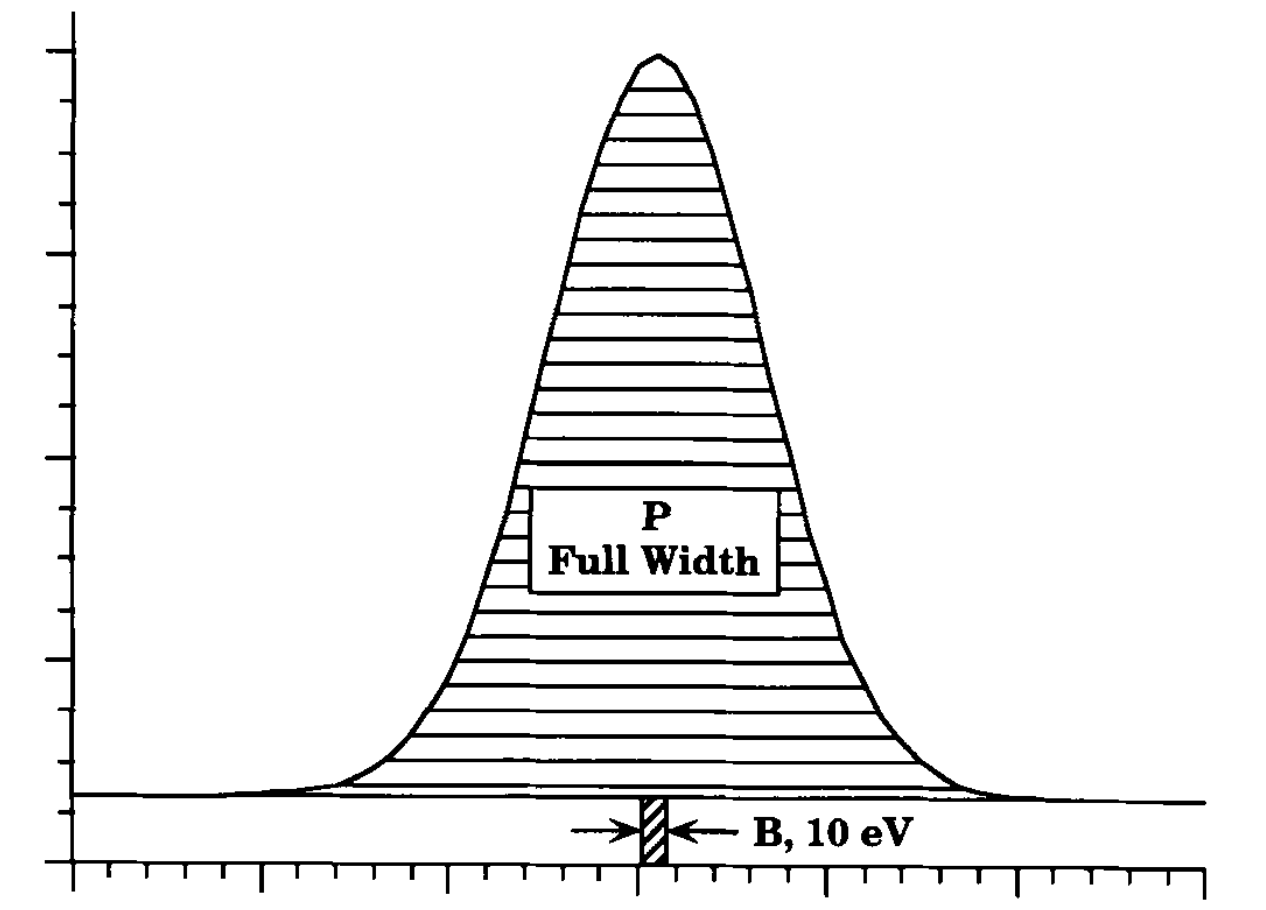
\includegraphics[width=0.6\linewidth]{figures/FioriPB_TODO_remake.png}
    \caption{
        Illustration of the Fiori P/B.
        P is all the counts in the actual peak, i.e. the part with the horizontal lines that does not including the background.
        B is the counts in a 10 eV window at the peak center.
        Figure adapted from \cite{zemyan_standard_performance_1994}.
        \brynjar{TODO: remake this figure. Uniform layout.}}
    \label{fig:fiori_pb}
\end{figure}

% How (and that is the issue)
% Issue with Fiori, the calculation
Even though the definition of the Fiori P/B is simple, the actual calculation of the metric is confusingly described slightly different in different sources.
Calculating the metric the same way is critical for comparing the results on different setups.
% The area of the peak is defined as the integrated counts above the background, because this was the best way to define the area of the peak in the 1970s, when the metric was first defined.
When the metric was developed, model fitting of the spectrum was not as trivial as it is today, and thus integration windows had to be used to estimate the peak and the background.
In the 1986 paper by Williams, the background B can be estimated by peak subtraction after using library standard, or B can be calculated with the specimen used as its own standard.
Using the specimen as its own standard seems to be the common way of calculating the B.
This is the way Zemyan and Williams define B in their 1994 paper \cite{zemyan_standard_performance_1994}, illustrated in  \cref{fig:fiori_pb_reality}, adapted from their paper.
The figure illustrates one of the ways to calculate the P and B: the background is estimated as the average counts in two integration windows before and after the peak divided by the number of channels, and the peak is estimated as the integrated counts minus the averaged background.
% Without the possibility of fitting the spectrum to a model, the method with the integration windows is the only way to calculate the Fiori P/B.




% figures/FioriPB_reality_TODO_remake.png
\begin{figure}[htbp]
    \centering
    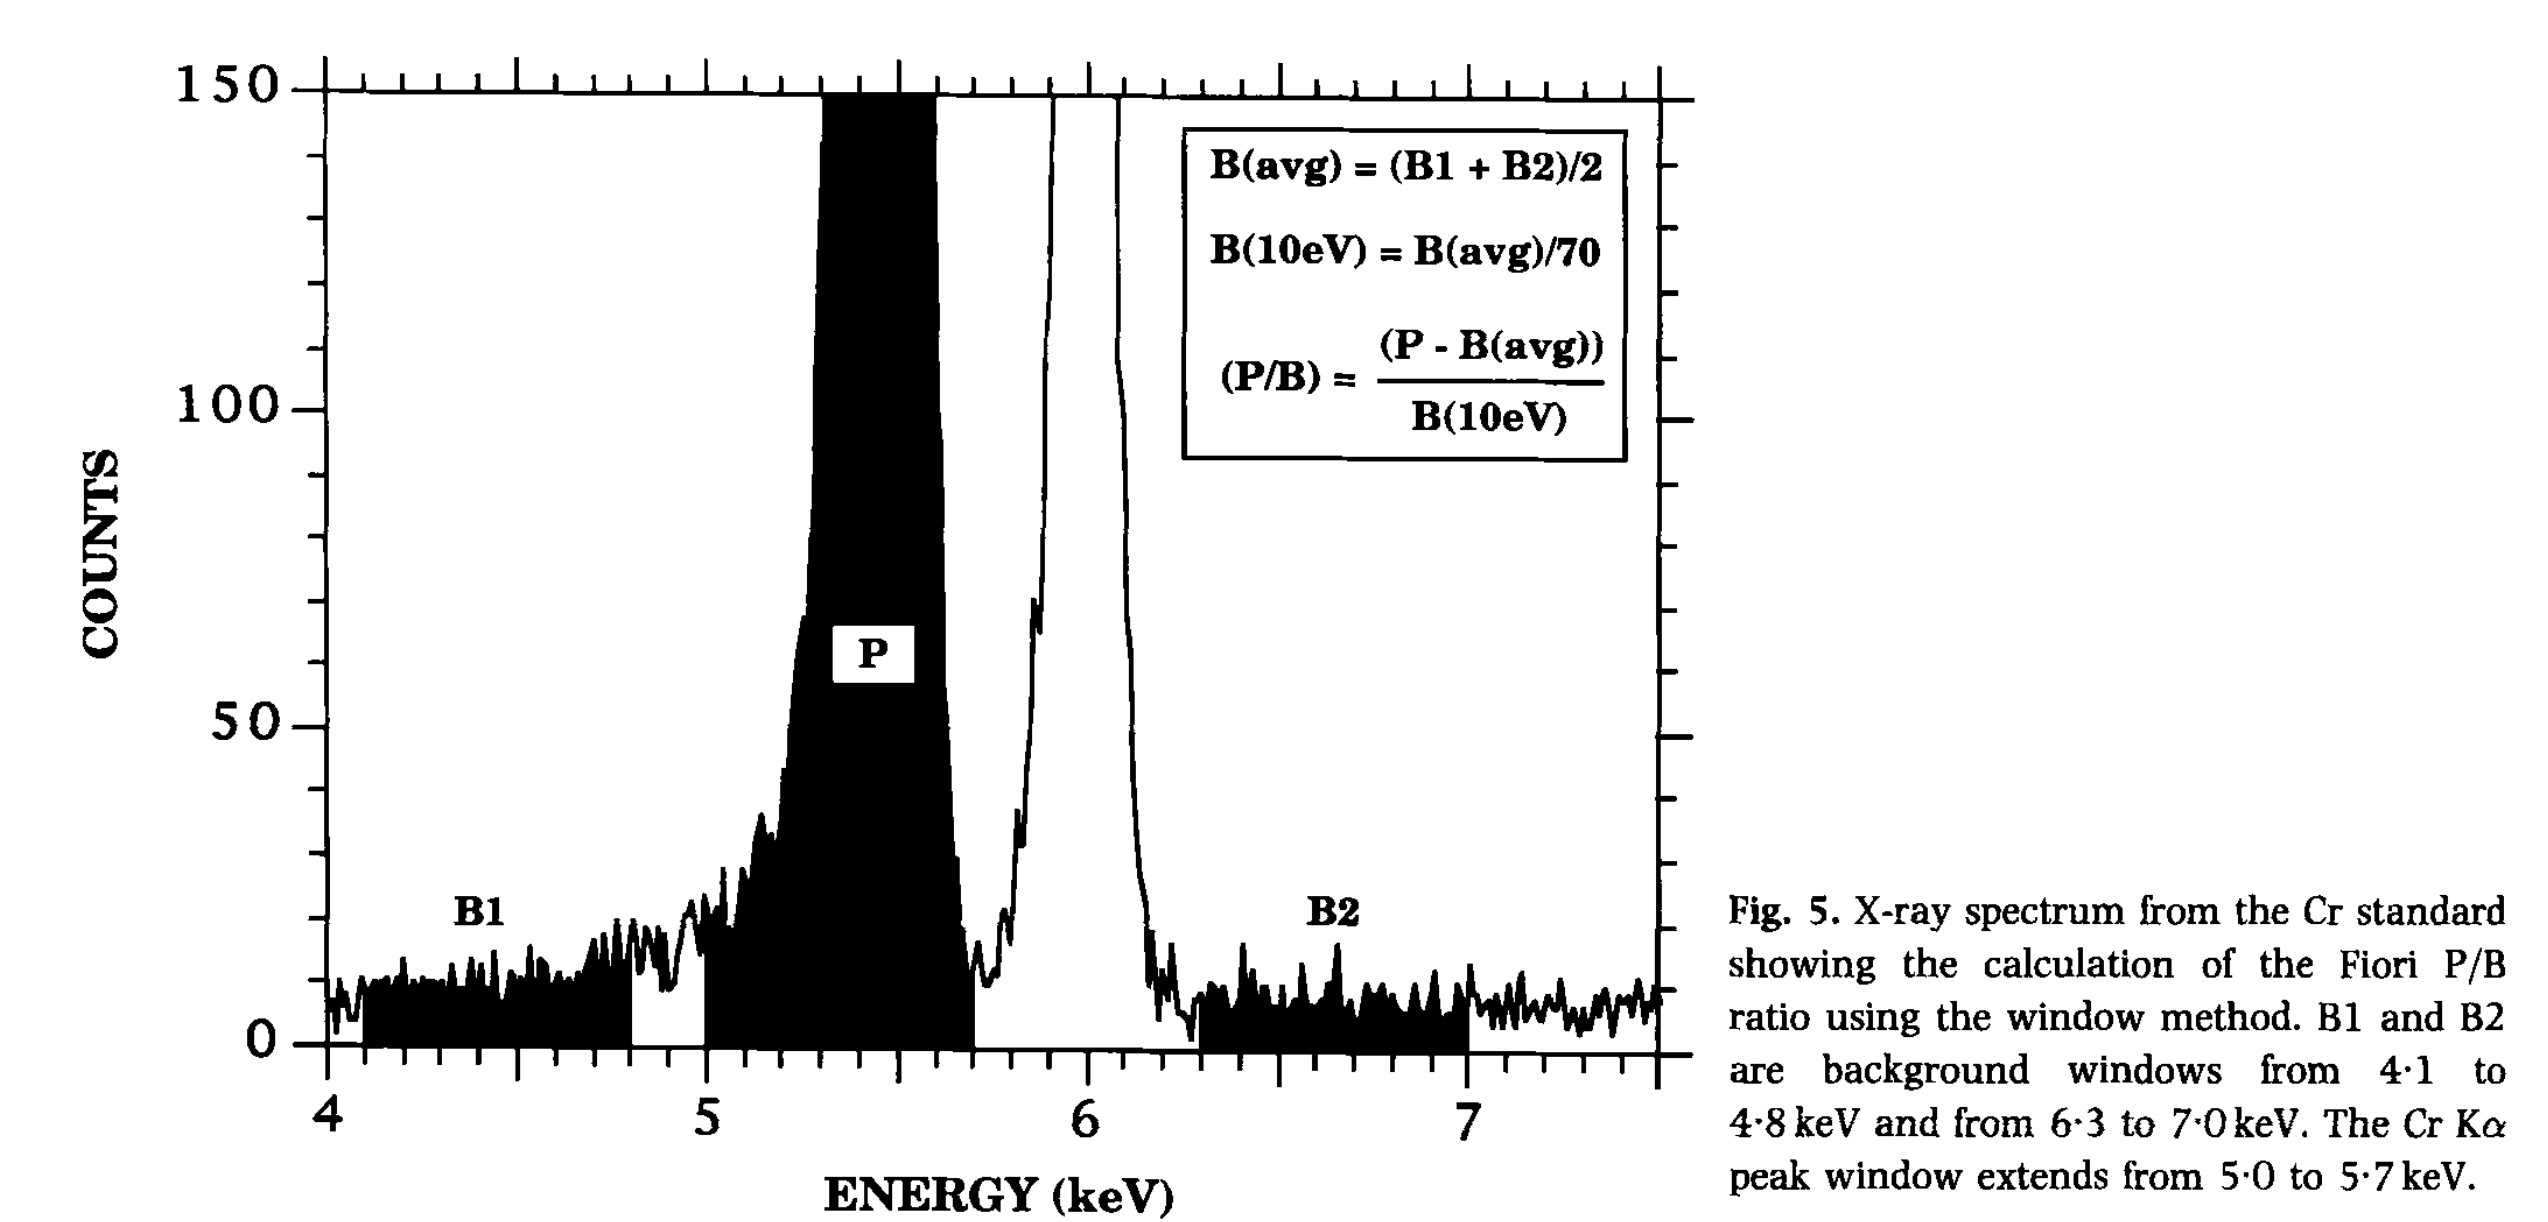
\includegraphics[width=0.6\linewidth]{figures/FioriPB_reality_TODO_remake.png}
    \caption{
        Illustration of how the Fiori P/B is calculated in practice, with integration windows.
        Figure adapted from \cite{zemyan_standard_performance_1994}.
        \brynjar{TODO: remake this figure?}
    }
    \label{fig:fiori_pb_reality}
\end{figure}


% using integration windows
Since the use of integration windows have to be done manually, the robustness of the metric is lowered.
The user must set the integration windows so that they do not include any other minor peaks, the background windows must be close enough to the peak so that the averaged background represents the background under the peak well enough, and the integration window of the peak must include the counts in the peak, but not include counts from other peaks.
Where the peak starts and ends is a subjective choice, and will vary between users.
Giving hard thresholds in energy is not an ideal solution, as the broadening with different settings can make an unwanted peak to "bleed" into an integration window.
% Different materials
The different integration windows specified are probably due to different materials used for the test.
The integration windows have to be adapted to the material, as suggested test materials can have other peaks close to the main peak, e.g. the peak between "P" and "B2" in \cref{fig:fiori_pb_reality}.
The topic of choosing a test material is part of the discussion in \cref{ch:discussion}.



% Something about overlapping peaks, like in the illustration which probably have a minor peak at the left side?
The problem with subjective choice of integration window, because of the lack of an agreed test standard \cite{williams_standard_definitions_1986}, is exemplified in the EDAX Insight newsletter from September 2018 \cite{edax_insight_2018}.
The newsletter contain an illustration of the Fiori P/B where the background windows are > 2 keV away from the peak.
This choice is not in agreement with their reference.
The widths of the integration windows are also varying in different papers, which probably does not affect the results too much as the background is converted to an estimate for a 10 eV window, but it is not ideal.
In EDAX Insight a 300 eV window is used for each background area far from the peak, but the paper that they refer to uses two 500 eV window directly before and after the peak \cite{egerton_nio_characterization_1994}.
For calculation of P, the Zemyan and Williams paper from 1994 use a 700 eV window \cite{zemyan_standard_performance_1994}, and the Ted Pella info-sheet on their NiO standard sample uses a 600 eV window \cite{ted_pella_nio_tem_2019}.
This is probably a result of different materials, i.e. Cr and Ni, having different peak widths, but it is not ideal for comparison.
The inconsistency of the actual calculation of the Fiori P/B is a problem for the metric.
This problem could be solved by fitting the spectrum to a model, and using the fitted curves to calculate the P and the B, to easily compare reported or claimed values from different set-ups.
This would make the metric truer to the original definition, and make it more robust as the users subjective opinions does not affect the calculation, and results from different materials might be more comparable.
This option is explored in this work.
% TODO: In discussion debate this choice to alternatives.





% Acceptable range
There are some papers \cite{egerton_nio_characterization_1994,egerton_nio_characterization_1994,ted_pella_nio_tem_2019} suggesting acceptable thresholds for the Fiori P/B, but they are for TEM EDS spectra.
It is stated in Williams and Carter \cite[p. 614]{williams_carter_tem_2009} that in a well constructed AEM the Fiori P/B ratio should increase with increasing beam energy.
% "In a well-constructed AEM, the P/B ratio will increase with keV." (Williams and Carter, p.614)
This should probably be true for SEM EDS setups too, and it is explored in this work.
% TODO: results and discussion on this
TEM EDS signals can have lower relative background intensity compared to SEM EDS signals, because the specimen is thin for TEM as explained in \cref{theory:sem:tem}.
This implies that a threshold should be lowered for SEM EDS signals.
Egerton and Chengs paper from 1994 \cite{egerton_nio_characterization_1994} suggests that a good TEM setup with a good signal have a Fiori P/B above 3000, while a number under 1000 indicates a bad signal.
Such high numbers might be too high for SEM EDS signals, but it is not clear what the threshold should be.
Additionally, the as the P scales with the composition and element, the threshold should be related to the composition and material.
As the Fiori P/B is dividing the total area of a peak, which typically spans 20-60 channels with 10 eV/channel, while the background is only from one channel, the metric should be a high number.
It might be that the threshold should be related to the specific detector, as detectors have a different background intensity.
Another potential use of the metric is to optimize the acquisition settings for specific specimen.
Higher numbers indicate a better signal-to-noise ratio, which should allow for better quantification of the specimen.
This is explored and focused on in this work, rather than trying to find a specific SEM threshold for the Fiori P/B.


% skrive om de forskjellige som finnes, og hvordan de varierer. Variasjon er ikke bra from sammenlikning
% visualisere hva jeg gjør


% fra møte 5:
% varierer med %-composition
% ulik definisjon gjør at verdiene ikke kan sammenliknes. 

% EDAX: https://www.edax.com/-/media/ametekedax/files/news_events/insight_newsletter/edax-insight-vol-16-no3.pdf?la=en&revision=d212987b-0524-4056-939e-858c59d06446
% TED PELLA: file:///C:/Users/Brynjar/Documents/Masteroppgave/potensielle%20kilder/Ted%20Pella%20NiOx%20description.pdf




\subsection{Peak ratios - carbon contamination and stray radiation}
\label{theory:eds_performance:peakratio}

A peak ratio, i.e. the counts in one peak divided by the counts in another peak, can be used to discover different issues with a detector.
\cref{tab:theory:lineEnergies} show the theoretical ratios inside families, i.e. between $\alpha$ and $\beta$ lines, but not the ratio between K and L.
Theoretical ratios between K and L can be found in the X-ray Data Booklet \cite{thompson_x-ray_2004}.
Egerton and Cheng \cite{egerton_nio_characterization_1994} show that a change in the ratio of the Ni K$\alpha$ to the Ni L$\alpha$ peak can be used to discover hydrocarbon contamination and icing of the detector.
The latter is not an issue with the newer SDDs, as they are not cooled down with liquid nitrogen.
The Ni K$\alpha$ line is at 7.48 keV, while the Ni L$\alpha$ line is at 0.85 keV, the latter being closer to the C K absorption edge, resulting in a higher sensitivity to hydrocarbon contamination.
Other peaks could also be used for this purpose, as long as one is close and above the C K$\alpha$ line and the other is far above.
The Ted Pella Info sheet \cite{ted_pella_nio_tem_2019} contains a formula for calculating the thickness of the contamination layer, but the assumptions used are not valid for SEM EDS signals.
A good reference numbers have not been identified for this metric for SEM EDS, and will depend on the chosen test specimen.
% TODO: you can discus this for the samples you have data on and suggest improvements on this aspect in the discussion chapter
However, detecting the contamination can be done by comparing a K/L peak ratio over time, where a decrease is an indication of carbon contamination.


Another use of peak ratios is to give information about the stray radiation.
This requires a specimen with a certain geometry, more specifically a specimen where the beam can be directed at one point with certain elements, and electrons deflected from the beam and secondary fluorescence happens at another area with different elements.
An example of such a specimen is a thin film on a substrate with a TEM grid pattern suspending the film, for example the NiO thin film on a Mo TEM grid from Ted Pella.
The beam is directed at the thin film, and the strays are recorded from the grid.
Two different metrics can be determined from such a specimen: (i) the intensity of the strays, and (ii) the predominant source of the strays.
(i) The intensity of the strays is given by the ratio of Ni K$\alpha$ peak to Mo K$\alpha$ peak.
An ideal setup have zero intensity in the Mo K$\alpha$ peak.
The stray radiations are unwanted signals, which can be a problem for quantification.
(ii) The predominant source of the strays is given by the ratio of Mo K$\alpha$ peak to Mo L$\alpha$ peak.
This is based on the assumption that the high energy Mo K$\alpha$ at 17.48 keV are generated by deflected electrons with a high energy, while the lower energy Mo L$\alpha$ at 2.29 keV are primarily generated by secondary fluorescence.
Both X-ray photons from background radiation and other elements can excite the Mo L$\alpha$ line, but the Mo K$\alpha$ line is almost only excited by electrons with a high energy, as the background is low at higher energies.
% contaminations, at least for TEM: change of Ka/La, eg in Ni
% also used for stray radiation measurements 
% stray intensity: (Ni Ka/Mo Ka) 
% stray predominent source: (Mo Ka/Mo La), only for TEM?

% the flexibility, since eg a pure Cu sample will give some statistics but not stray information.


% \subsection{Peak shape}
% \label{theory:eds_performance:peakshape}
% % The real lines are Lorentzians with width of 1-10 eV, but the peaks are wider due to electronic noise.
% % Peaks are gaussians by electronic noise.
% % a measure of the peak shape is the FWTM/FWHM

% Could be used to see overlapping peaks, or for misidentification of peaks.


\subsection{Total counts and background portion}
\label{theory:eds_performance:background_portion}

\brynjar{Comment from Ton: "should this section not be incorporated in the Fiori section or placed directly after it?" Yes, that is a good idea.}

% Total counts, background counts.
% How to represent the measure better? Ratio, percentage, absolute value, etc.
% Fiori P/B is a measure already covered.

As EDS vendors tend to be eager to report high count rates, it might prove useful to look at the total counts in a spectrum.
The background portion is simply the percentage of the total counts that are from the background.
This is a metric that can be used to optimize the acquisition settings for a specific specimen, for example to find optimal beam energy and current.
As the background portion will vary with specimen and detectors, no specific value can be given for a good background portion.

% formula
\begin{equation}
    \label{eq:theory:eds_performance:background_portion}
    \frac{\textnormal{Background counts}}{\textnormal{Total counts}} \times 100\%
\end{equation}


The variation in background is affecting the Fiori P/B, as illustrated in \cref{fig:theory:eds_performance:overview:fiori_snr}.
Having both the Fiori P/B and the background portion as metrics might be redundant.
The usefulness of using both metrics is explored further in this work.




% One example of the usefulness of the background portion is when the specimen is absorbing most of the signal, as was the case in one of the spectrum in the authors previous work \cite{project_report}.
% This is shown in \cref{fig:theory:eds_performance:background_portion:poor_Cu_tape}.
% Here the two spectra is shown from a Cu-tape, where the sticky tape part was not removed.
% The 10 kV spectra had almost no counts compared to the 30 kV spectra, except for the C K$\alpha$ peak.
% Even the background was very low in the 10 kV spectra.
% This gives a very high Fiori P/B metric for the C K$\alpha$ peak in the 10 kV spectra, even though the spectrum is of poor quality.
% The low background signal is due to the absorption of the X-rays by the sticky tape part, assumed to be carbon.
% Lower acceleration voltage give shallower escape depts, e.g. in C the escape depth for Cu K$\alpha$ 414 nm at 10 kV and 7620 nm at 30 kV \cite{hyperspy_1.7.1}.
% Other X-ray photons follow the same logic, e.g. less signal being emitted from C when using lower acceleration voltage.
% The 10 kV spectrum have an extraordinarily low background portion, which should raise a red flag for the quality of the spectrum.
% \brynjar{Give numbers here?}




\begin{table}[htp]
    \centering
    \caption{
        Summary of the performance parameters covered in this thesis.
    }
    \renewcommand*{\arraystretch}{1.4}
    \label{tab:eds_performance_parameters}
    \begin{tabular}{p{2.5cm}p{8cm}p{3.5cm}}
        \hline
        \textbf{Parameter}                                                          & \textbf{Definition}                                                                                                                                                                                                                                         & \textbf{Characterizes}                                             \\
        \hline
        \hyperref[theory:eds_performance:duanehunt]{Duane-Hunt limit}               & The effective incident beam energy, i.e. the maximum energy generating X-rays. Found by linear regression \cite{Duane_Hunt_1915,software_dtsaii,goldstein_scanning_2018}. See \cref{fig:duanehunt}.                                                         & Charging issues and verifies the selected $E_0$.                   \\
        \hyperref[theory:eds_performance:energyres]{Energy resolution}              & Measured as the FWHM(Mn K$\alpha$). Can be measured directly or calculated with \cref{eq:estimateFWHM} \cite[Ch. 16.1.1]{goldstein_scanning_2018}. $\textnormal{FWHM}(E) =  \sqrt{2.5 * (E - E_\textnormal{ref}) + \textnormal{FWHM}^2_{\textnormal{ref}}}$ & The detector specifications and the settings used for acquisition. \\
        \hyperref[theory:eds_performance:scaleoffset]{Scale and offset}             & The width of each channel and the zero-offset of the spectrum.                                                                                                                                                                                              & The settings selected by the user.                                 \\
        \hyperref[theory:eds_performance:scaleoffset]{Deviations in peak positions} & How many eV the center of the fitted Gaussian deviate from the theoretical peak center.                                                                                                                                                                     & The accuracy of the electronics.                                   \\
        \hyperref[theory:eds_performance:fiori]{Fiori P/B ratio}                    & A signal-to-noise ratio. The sum of all the counts in a peak divided by the background counts in a 10 eV window under the peak center  \cite{fiori_peak_background_1982,williams_carter_tem_2009}. See \cref{eq:fiori_pb} and \cref{fig:fiori_pb}.          & The detector quality and quality of the acquired spectrum.         \\
        \hyperref[theory:eds_performance:peakratio]{Peak ratios}                    & Counts in one peak divided by the counts in another peak. With specific specimen geometry, this can be used to characterize strays. \cite{egerton_nio_characterization_1994,ted_pella_nio_tem_2019}.                                                        & Information about stray radiation, and carbon contamination.       \\
        % \hyperref[theory:eds_performance:background_portion]{Background portion}      & The percentage of the total counts which are from the background.                                                                                                                                                                                           & The quality of the acquired spectrum.                              \\
        \hline
    \end{tabular}
\end{table}


% TODO 
% \ton{Everything above this page is more or less finished now. How would you rate it?}
% It is good, detailed. The visualizations/figures are very useful for the reader, the summarizing tables not always.
% Some points are repeated and as long (but keep as it is now!) less interested reader could loose the red line. 
% Use the theory when discussing your own results and finding, refer to theory and use in the discussion the reference you use here. Debate your choices to use a certain approach/criteria and compare to what if another is used. 
% Theory is detailed, backup and now you have to integrate it/ use it in the discussion part to have a interlinked report.




\clearpage





































% Issue with matrix correction: 

% Matrix correction, ASTM 1508:
% 10.2.1 "If the unknown and standard were
% identical, each of these factors would equal one. There are
% many such “ZAF” computer programs available,[...].
% The differences in the results each produces are usually
% much less than the precision of the analysis."
% 10.2.2 "10.2.2 There are also many computer programs using the“
% phi-rho-z” method.  These approach the problem of matrix
% correction using more fundamental physics and sometimes
% combine the effects of Z and A into one, but they too require a
% set of fundamental parameters optimized to each program.
% Many phi-rho-z programs claim greater accuracy because they
% account for absorption better than the older ZAF programs.
% Consequently, one would expect the most improvement using
% a phi-rho-z method in light element analysis. However, in the
% absence of light elements, it is unlikely that the accuracy of
% most EDS analyses is limited by the matrix correction."






\section{Quantitative EDS analysis}
\label{theory:quantitative}



\brynjar{TODO: Fjerne det om phi-rho-z, fordi jeg bruker PAP/XPP, og vurderte å bruke PROZA96}


% Limitations done in this work
This work aims to improve the analysis for SEM EDS data, and this section will focus on the quantitative analysis, a part of the third area of improvement, illustrated in \cref{fig:intro:parameters}.
% As a master thesis, the scope of this work is limited, and 
The hypothesis is that for bulk specimens matrix corrections have to be incorporated in the quantifications routines.
The focus within the quantitative analysis has thus been to implement matrix corrections in a Jupyter notebook which could be developed further, for example as an addition to the HyperSpy package.
As stated in the ASTM 1508 standard \cite{astm_e1508_eds_quantification}, there are multiple different programs available for matrix corrections with some differences, but the accuracy of the EDS analysis is probably not limited by the accuracy of the matrix correction \cite{astm_e1508_eds_quantification}.
The two matrix correction methods explored and tested in this work are (1) absorption correction through ZAF corrections, and (2) the XPP version of the PAP algorithm \cite{pap_1991}.
These two methods are introduced below.
This section will start with an introduction to the principle of quantitative EDS analysis, before the two correction methods are presented.






\subsection{Principle}
\label{theory:quantitative:principle}

The principle of quantitative EDS analysis was introduced by Castaing in 1951 \cite{castaing_1951}, where he showed that quantitative data could be obtained by comparing the X-ray intensity from element A in an unknown sample to the same intensity in a sample with a known concentration of element A.
The known sample is referred to as the standard, and was frequently selected to be pure elements for convenience.
Using the same instrumental conditions on the known and the unknown, Castaing showed that the \emph{generated intensity} ratio can be related through the \emph{mass concentration} ratio of the two samples, as shown in:

% C_unknown / C_standard = I_unknown / I_standard

\begin{equation}
    \label{eq:theory:quantitative:castaing_generated}
    \frac{C_\textnormal{unknown}}{C_\textnormal{standard}} = \frac{I_{0\textnormal{, unknown}}}{I_{0\textnormal{, standard}}}
\end{equation}

Where the $C$ is the mass concentrations and the $I_0$ is the generated intensity\footnote{It is common to note the unknown as $i$ and the standard as $(i)$, but the more explicit notation is used in this work for clarity.}.
However, the generated intensity is not the same as the measured intensity, thus Castaing introduced a sensitivity factor applied to the measured intensity ratio:

% C_unknown / C_standard = k * I_unknown / I_standard

\begin{equation}
    \label{eq:theory:quantitative:castaing_measured}
    \frac{C_\textnormal{unknown}}{C_\textnormal{standard}} = K \frac{I_\textnormal{unknown}}{I_\textnormal{standard}}
\end{equation}

Where $I$ is the measured intensity and $K$ is a sensitivity factor that depends on the atomic number (Z), the absorption (A), and the fluorescence (F) in the sample \cite{goldstein_scanning_2018,williams_carter_tem_2009}.
% These corrections for bulk specimen is covered below.
The implementation of satisfactory sensitivity factors is a complicated task, as the X-rays are generated in an interaction volume which depends on the specimen composition and the electron probe conditions.
Castaing and Deschamps established the theory experimentally in 1955, but the method was restricted by the sensitivity calculation as an iterative process. %  \cite{castaing_1955},
Later Philbert derived an analytical expression for iterative routines \cite{philbert_1963}.
Now there are two main groups for the matrix corrections: the ZAF-corrections and the $\phi(\rho z)$-corrections.
ZAF-corrections treat Z, A, and F independently, and is covered in \cref{theory:quantitative:zaf}.
The $\phi(\rho z)$-corrections treat the Z and A together in a more complex calculation, and is covered in \cref{theory:quantitative:pap}, as a part of the PAP algorithm\footnote{Algorithm, model, and principle is used interchangeably in this work.}.
The $\phi(\rho z)$ curve is the depth distribution of radiation from a certain X-ray line as a function of mass depth ($\rho z$), i.e. the curve describes how much of the generated X-rays that is emitted from a certain level in the sample.


% The Cliff-Lorimer method, for thin samples
One way to avoid the corrections and thus also avoid the iterative process is to use thin samples.
In thin samples the absorption and fluorescence can be neglected, which is typically the case for TEM specimen.
Cliff and Lorimer \cite{CL1975} showed in 1975 that the intensity from a specimen with two elements can give the composition ratios, without the use of standards.
The Cliff-Lorimer method have a sensitivity factor which is dependent on the instrument settings and the atomic number effects in the specimen.
This sensitivity factor in the Cliff-Lorimer method is named the "k-factor".
The Python package HyperSpy have the Cliff-Lorimer quantification method implemented.
Additionally, HyperSpy have implementations of the Zeta method \cite{watanabe_williams_zeta_2006} and the cross-section quantification approach \cite{MacArthur}.
Absorption corrections for TEM specimen is also implemented as a optional part of the quantification routines in HyperSpy for TEM specimen.
These absorption corrections are based on path length and found composition \cite{williams_carter_tem_2009}.
\ton{Based on your comment, should I add: "The TEM EDS routines in AZtec are hidden, but the software probably use the Cliff-Lorimer method, and might have some implementation of TEM absorption correction."?}


\ton{These two eq and three paragraphs are new. I call it the "area ratio method".}

% The area ratio of two similar peaks
When relative quantification is sufficient, the area ratio of two similar peaks can be used \cite{goldstein_scanning_2018}.
When using measured standards, the absolute concentrations can be obtained.
Using the absolute concentrations can reveal errors in the analysis, as the summed concentrations should be close to 100\% \cite{goldstein_scanning_2018}.
However, using relative concentrations requires less work, and is probably the most common method for EDS analysis \brynjar{[citation needed]}.
Similar peaks are peaks which emit similar amounts of X-rays, for example having X-ray energy not too far apart, having similar fluorescence yield (\cref{fig:theory:fluorescence_yield}), and having similar absorption (\cref{fig:mass_absorption_coefficients}).
If the emitted amount of X-rays are similar, the relative composition can be calculated with:

% C_A = I_A / (I_A + I_B)
\begin{equation}
    \label{eq:theory:quantitative:area_ratio}
    C_A = \frac{I_A}{I_A + I_B}
\end{equation}

Where $C_A$ is the concentration of element $A$, and $I_A$ and $I_B$ is the measured intensity in a peak from element $A$ and $B$ respectively.
The concentration from such calculations are in weight percent (wt\%).
If the lines used emit different amounts of X-rays, a sensitivity factor can be applied to the measured intensity ratio.
The sensitivity factor can take into account the atomic number, the absorption, and the fluorescence in the sample.
Depending on the specimen and acquisition parameters, it might be sufficient to use a sensitivity factor that only focus on a specific parameter.
For example, if the Z of the elements are close, the sensitivity factor can be based on the absorption, if absorption is the dominating factor.
The equation then becomes:

\begin{equation}
    \label{eq:theory:quantitative:area_ratio_corrected}
    C_A = \frac{k_A \cdot I_A}{k_A \cdot I_A + k_B \cdot I_B}
\end{equation}

Where $k_A$ and $k_B$ is the sensitivity factors for element $A$ and $B$ respectively.
This method is referred to as the "area ratio method" in this work, without and with corrections.




% \subsubsection*{Side note: Two definitions of the ZAF-method}

As explained in chapter 19.10.1 in Goldstein, there are two definitions of the ZAF-correction method, which are inverses of each other.
The first definition ($ZAF_A$) applies the corrections to the concentration, and the second definition ($ZAF_B$) applies the corrections to the intensity.


\begin{equation}
    \label{eq:theory:quantitative:zaf_a}
    \frac{I_\textnormal{i, unknown}}{I_\textnormal{i, standard}}  = \frac{C_\textnormal{i, unknown}}{C_\textnormal{i, standard}}\cdot ZAF_A
\end{equation}

\begin{equation}
    \label{eq:theory:quantitative:zaf_b}
    \frac{C_\textnormal{i, unknown}}{C_\textnormal{i, standard}} = \frac{I_\textnormal{i, unknown}}{I_\textnormal{i, standard}} \cdot ZAF_B
\end{equation}

The two definitions are related by the following equation:

\begin{equation}
    \label{eq:theory:quantitative:zaf_a_b_relation}
    ZAF_A = \frac{1}{ZAF_B}
\end{equation}

Relevant for this work is $ZAF_B$.





\subsubsection*{Side note: The difference between the k-factor and the k-ratio}
\label{sec:theory:quantitative:k_factor_vs_k_ratio}

\brynjar{TODO, from Ton: "Yes, but not here. Introduce ratio from formulas above or from Goldstein and than compare the two as a halfway summary."}

The \textbf{k-factors} are a sensitivity factor used in the Cliff-Lorimer quantification method for thin samples \cite{CL1975,williams_carter_tem_2009}.
The value of the k-factor is dependent on the instrument setup and the acceleration voltage.
\brynjar{From Ton: "could give the formula for the k-factor, Williams and Carter give it for example, and than discus that it has a set-up part (detector size, efficiency) and a physics side (cross section for processes)"}.
The Cliff-Lorimer method relates atom $A$ to atom $B$ in a sample with the following equation:

\begin{equation}
    \label{eq:theory:quantitative:cliff_lorimer}
    \frac{C_A}{C_B} = k_{AB} \frac{I_A}{I_B}
\end{equation}

Where $k_{AB}$ is the k-factor for the two elements $A$ and $B$.
The k-factor is most accurately determined experimental, but can be calculated theoretically.
The Cliff-Lorimer method use the thin film approximation, where the absorption and fluorescence can be neglected.
In other words, the k-factors are only used for thin samples.


When quantification of bulk samples is needed, the \textbf{k-ratio} method can be used to get an estimate of the composition \cite[Ch. 19.1]{goldstein_scanning_2018}.
The k-ratio is the ratio between the measured intensity of an unknown and a standard, where ideally all other parameters and factors than the composition is the same.
The estimate of the composition from the k-ratio can be paired with matrix corrections to give a more accurate composition.
The k-ratio of element $i$ is defined as:

\begin{equation}
    \label{eq:theory:quantitative:k_ratio}
    k_i = \frac{I_\textnormal{i, unknown}}{I_\textnormal{i, standard}}
\end{equation}


To get the more accurate composition through the k-ratio, the ZAF-corrections can be used.
The corrections must be applied to both the unknown and the standard, and the composition of the unknown can be found through the equation:

\begin{equation}
    \label{eq:theory:quantitative:k_ratio_ZAF}
    C_\textnormal{i, unknown} = C_\textnormal{i, standard} \cdot  \frac{(I \cdot ZAF)_\textnormal{i, unknown}}{(I \cdot ZAF)_\textnormal{i, standard}} = C_\textnormal{i, standard} \cdot k_i \cdot \frac{(ZAF)_\textnormal{i, unknown}}{(ZAF)_\textnormal{i, standard}}
\end{equation}

The ZAF corrections are a function of the concentration of the element, and thus the ZAF-corrections must be applied iteratively with an initial guess of the composition of the unknown.
As with the k-factor, the k-ratio is most accurately determined experimentally, but can be calculated theoretically.
The AZtec software from Oxford Instruments \cite{aztec_manual} can both provide the k-factor and the k-ratio for the elements in an analyzed sample, which are theoretically calculated.










\subsection{ZAF absorption correction}
\label{theory:quantitative:zaf}

The part of the ZAF corrections tested in this work are the absorption corrections.
The atomic number correction (Z) in ZAF is excluded, as it is stated in Goldstein that the correction effects which tend to go in opposite directions and cancel each other out \cite[p. 300]{goldstein_scanning_2018}.
These two effects are the backscattering factor (R) and the stopping power (S).
Both R and S is implemented in the PAP model \cite{pap_1991}, which is claimed to be more accurate than the ZAF method \cite{pap_1991,bastin_proza96_1998,goldstein_scanning_2018}
The fluorescence correction (F) is excluded, because it is stated in Goldstein that this correction is usually the least important one \cite[p. 307]{goldstein_scanning_2018}.
The low importance of the F correction is illustrated in figure 6 in P. Burdets publication on 3D SEM EDS \cite{burdet_2014_3dsem}.
The generated intensity is reduced before detection due to absorption in the specimen.
The absorption reduces the measured intensity of X-rays from a certain point by:

% I = I_0 * exp(-mu * rho * t)
\begin{equation}
    \label{eq:theory:quantitative:absorption}
    I = I_0 \cdot e^{-\mu_{\rho} \cdot \rho \cdot t}
\end{equation}

Where $I$ is the measured intensity, $I_0$ is the generated intensity, $\mu_{\rho}$ is the mass absorption coefficient\footnote{Again, mass absorption coefficient is actually defined as $\mu/\rho$, but is written as $\mu_\rho$ in this work, because the mass absorption coefficient is treated as a single variable.},
%because writing $(\mu/\rho)\cdot \rho$ not ideal.}, 
$\rho$ is the density of the specimen, and $t$ is the path length of the X-ray in the specimen.
The unit in the exponential have to cancel out, thus one can use the following units: $I$ and $I_0$ in the same and arbitrary units, $\mu_{\rho}$ in $\textnormal{cm}^2/\textnormal{g}$, $\rho$ in $\textnormal{g}/\textnormal{cm}^3$, and $t$ in $\textnormal{cm}$.
$\mu_{\rho}$ is explained in \cref{theory:xray_formation:characteristic} and plotted in \cref{fig:mass_absorption_coefficients,fig:background_absorptionEdgeSi}
As the detector is placed at a certain angle, the take-off angle, the path length becomes:

% t = z *csc(TOA)
\begin{equation}
    \label{eq:theory:quantitative:path_length}
    t = z \cdot \csc(\textnormal{TOA})
\end{equation}

Where $z$ is the depth of origin of the X-ray, TOA is the take-off angle, and csc is the cosecant function.
Tilting the specimen will change the path length of the X-ray, and thus the absorption.


% calculating I_0 from an average point or for the whole interaction volume
The most correct use of the absorption correction is to calculate the absorption for each point (or layer) in the interaction volume, which is usually done through $\phi(\rho z)$ curves.
This calculation is part of the PAP method described in \cref{theory:quantitative:pap}.
For the ZAF method used in this work, the absorption correction is calculated for an average point in the interaction volume.
The average point selected is the maximum path length of an incident electron, divided by two, three or four.
\brynjar{Results: Add r/2, r/3, r/4 to the results.}
The electron range is calculated with the Kanaya-Okayama parameterization \cite{kanaya1972}, which is available in HyperSpy \cite{hyperspy_1.7.1}.
The Kanaya-Okayama parameterization is given in Goldstein as \cite[22.5]{goldstein_scanning_2018}:

\begin{equation}
    \label{eq:theory:quantitative:kanaya_okayama}
    R_{K-O} [\mu m] = (0.0276 A / Z ^{0.92} \rho) \cdot (E_0^{1.67} - E_C^{1.67})
\end{equation}

Where $A$ is the atomic weight in g/mol, $Z$ is the atomic number, $\rho$ is the density in g/cm$^3$, $E_0$ is the incident electron energy in keV, and $E_C$ is the critical ionization energy in keV.
The equation is made for pure elements, but in this work the average $A$, $Z$ and, $\rho$ of the elements in the sample is used.
In Goldstein, Eq. 14.1 gives the $R_{K-O}$ in a specimen without the correction for $E_C$.
The range $R_{K-O}$ calculated the equation use the critical ionization energy as a threshold, because electrons with energy lower than this is not of interest.
Using for example $R_{K-O}/2$ as the average point for the generated intensity is an approximation which can give a reasonable result, at least it should be in the correct order of magnitude.
\brynjar{To discussion and results: maybe this approximation is severely wrong. Monte Carlo simulations show a skew towards z=0, and the numbers from HS is big. However, testing different numbers for r did not give any other more satisfactory results. Also, the phi-rho-z curves show that there is a skew towards z=0, at Rc.}
This simplification is partly justified by the fact that the available measured intensity $I$ is the sum of the intensity from all points in the interaction volume.
Testing out different methods with varying complexity for calculating the absorption correction is a step towards finding a suitable implementation for HyperSpy.
If a simpler model proves to be sufficient, it will allow users to understand the correction faster and possibly altering it to the specific needs, while also being easier to implement and maintain in HyperSpy.












\subsection{The PAP model}
\label{theory:quantitative:pap}

\brynjar{Unfinished. I use PAP or XPP, not PROZA96.}


Pouchou and Pichoir presented their PAP model for bulk corrections on a conference in 1983 and published a detailed paper about PAP in 1991\footnote{"PAP" is short for "Pouchou and Pichoir" \cite{pap_1991}.}.
The model is a mathematical heavy model which is physically based on X-ray generation and emittance, and the model should be able to correct for a wide range of compositions \cite{pap_1991}.
In the 1991 publication, a simplified model called XPP is also presented\footnote{"X" in XPP is probably short for e.g. express, but it is not stated in the paper.}.
Alternative methods exist for bulk corrections which produce similar results, but are mathematically different.
One example of such a model is the PROZA96 model, which is an iterative model which calculate the $\phi(\rho z)$ curve as a double Gaussian.
The PROZA96 model is published by Bastin, Dijkstra, and Heijligers in 1996, as an improvement to the same authors previous model from 1988 \cite{bastin_proza96_1998,bastin_proza_1988}.
The difference between the models is the calculation of the $\phi(\rho z)$ curves, where the PAP model use a linear combination of two exponential functions to calculate the $\phi(\rho z)$ curve, not a double Gaussian as the PROZA96 model or the Gaussian model from Packwood and Brown \cite{packwood_1981}.
As it is, allegedly, the XPP model which is used in AZtec \cite{} \brynjar{cite this correctly}\footnote{\url{https://www.oxinst.com/blogs/how-to-overcome-challenges-in-publishing-eds-results}}, it is the XPP model which is tested in this work.
Other methods, such as the PROZA96 model, could be tested in future works, using the code developed in this work as a starting point, because there are overlapping parts between the models.
Both the PAP and the PROZA96 model use the area of the $\phi(\rho z)$ curve for parameterization, where the PROZA96 model refers to the PAP paper for the calculation of this area \cite{bastin_proza96_1998}.
\brynjar{TODO discussion: advice future work to test the PROZA96 model, using my code as a starting point.}
At the end of the section, \cref{tab:quantitative:PAP:variables} summarize all the variables, with their name, their use, and their units.




% \begin{quote}
%     Quote from the PAP-paper:
%     \emph{"We believe that, rather than treating separately the improvement of corrections for
%         homogeneous specimens and the characterization of specimens of composition variable in
%         depth, it would be more logical and efficient to conceive a general and unique model for the
%         calculation of emergent x rays.
%         For this we have used the usual fundamental physical
%         concepts applied in x-ray microanalysis and we apply to them as accurate a description of
%         the depth distribution, $\phi(\rho z)$ as possible."}
% \end{quote}



The PAP model is a mathematical model which is based on the physics of X-ray generation and emittance.
It is a model which calculates the emergent X-rays based on the depth distribution of the generated X-rays, $\phi(\rho z)$, and the absorption of the generated X-rays at different depths.
The model gives correction for homogeneous specimens, and the paper describe how it can be applied to specimen with composition varying in depth, specimen with surface coating, and lighter elements \cite{pap_1991}.
The version which is discussed here is the model for homogeneous specimen.
\brynjar{TODO discussion: say something about specimen geometry, as was commented on the presentation.}


The $\phi(\rho z)$ curve gives the depth distribution of the generated X-rays in a bulk specimen relative to a thin specimen.
The curve is a function of mass depth ($\rho z$), where mass depth is the product of density ($\rho$) and depth ($z$) from the surface. 
The unit for the mass depth is $\textnormal{g}/\textnormal{cm}^2$.
The intensity from each layer is divided by the intensity from a similar, but thin, specimen.
As the bulk specimen have many backscattered electrons, which also generate X-rays, the $\phi(\rho z)$ curve has a distinct and general shape:
The curve starts above 1, increase to a maximum, and then decrease to 0.
Three $\phi(\rho z)$ curves are illustrated in \cref{fig:theory:quantification:phi_rho_z_curves}.
At the end of this section, $\phi(\rho z)$ curves are plotted with the equations from the PAP model.




% figures/phi_rho_z_curves__goldstein.png
\begin{figure}[htbp]
    \centering
    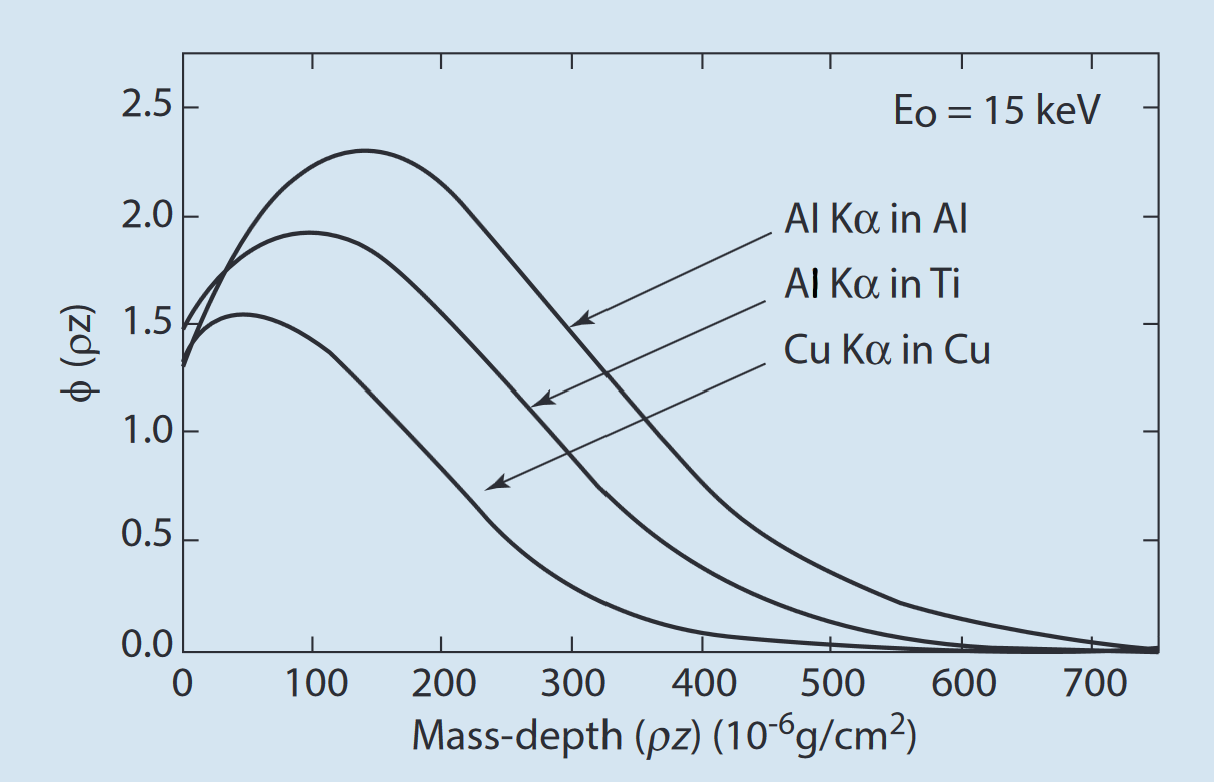
\includegraphics[width=0.65\linewidth]{figures/phi_rho_z_curves__goldstein.png}
    \caption{
        Three calculated $\phi(\rho z)$ curves.
        Al K$\alpha$ in Al and Ti, and Cu K$\alpha$ in Cu, calculated at 15 kV.
        The curves are calculated with the PROZA model \cite{bastin_proza_1988}
        Adapted from Goldstein \cite[Fig. 19.9]{goldstein_scanning_2018}.
        \brynjar{Is it supposed to be "Al Ka in Cu", not "Cu Ka in Cu", because of increased rho? Al Ka and Cu Ka have very different $E_C$.}
    }
    \label{fig:theory:quantification:phi_rho_z_curves}
\end{figure}


The following is a consice description of the PAP model, detailed enough to implement the model in a Jupyter Notebook. For further details, see the original paper \cite{pap_1991}, the fourth edition of Goldstein for a brief description \cite{goldstein_scanning_2018}, the second edition of Goldstein for a more detailed description \cite{goldstein_2ed_1992}, or \dots \brynjar{find more references, e.g. Reimer}.








\subsubsection{General principle of the PAP model}
\label{theory:quantitative:pap:general_principle}

The PAP model is in accordance with the original definitions from Castating.
The calculations done in the PAP model is divided into two parts: (a) find the the \emph{generated intensity} by calculating the area $F$ under the $\phi(\rho z)$ curve, and (b) calculate the \emph{emitted intensity} $F(\chi)$ based on a parabolic representation of $\phi(\rho z)$ with an absorption correction.
Both calculations are done analytically.
A summary of the variables in this principle part of the PAP model is given in \cref{tab:quantitative:PAP:variables:principle}.


\emph{The generated intensity}, or number of primary ionizations, of line $l$ in atoms of element A by the incident electron is given by:

% n_a = C_a N^0/A Q(U) F
\begin{equation}
    \label{eq:theory:quantitative:pap:general_principle:n_a}
    n_A = C_A \frac{N^0}{A} Q(U) F
\end{equation}

Where $n_A$ is the number of generated primary ionizations from atoms of element A, $C_A$ is the concentration of element A in weight percent\footnote{The author have had some frustrating moments because of mixing of wt\% and at\% while working with quantitative EDS.}, $N^0$ is Avogadro's number, $A$ is the atomic weight of element A\footnote{The author of this work assumes $A$ is the atomic weight, but it is not stated explicit in the PAP-paper.}, $Q(U)$ is the ionization cross section of the line with the given overvoltage ($U$)\footnote{$Q(U)$ is noted as $Q_l^A(E_0)$ in the PAP-paper.}, and $F$ is the integral of $\phi(\rho z)$.

% F = int_0^infty phi(rho z) dz
\begin{equation}
    \label{eq:theory:quantitative:pap:general_principle:F}
    F = \int_0^\infty \phi(\rho z) d\rho z
\end{equation}


\emph{The emitted intensity} from a specimen is given by:

\begin{equation}
    \label{eq:theory:quantitative:pap:general_principle:I_A}
    I_A \propto C_A \cdot Q(U) \cdot F(\chi)
\end{equation}

Where $I_A$ is the emitted intensity from element A, $C_A$ is the concentration of element A in mass concentration, $Q(U)$ is the ionization cross section, and $F(\chi)$ is the integral of $\phi(\rho z)$ with an absorption correction $\chi$.
$ \chi = \mu_\rho \cdot \csc(TOA)$\footnote{$\chi$ is not explicitly defined in the PAP paper, but is taken from Love and Scott \cite[Eq. (1)]{love_scott_1990}, which is a reference in the PAP paper.}.
This equation omits parameters which are equal or almost equal for the elements in the specimen, such as the solid angle of the detector, the electron flux, and the detector efficiency.


\begin{equation}
    \label{eq:theory:quantitative:pap:general_principle:f_of_chi}
    F(\chi) = \int_0^\infty \phi(\rho z) \cdot e^{-\chi \cdot \rho z} d\rho z
\end{equation}


The relation between the emitted and generated intensity will give the absorption correction $f(\chi)$:

\begin{equation}
    \label{eq:theory:quantitative:pap:general_principle:f_absorption_correction}
    f(\chi) = \frac{F(\chi)}{F}
\end{equation}





\begin{table}[phtb]
    \begin{center}
        \caption{
            Variables from the principle of PAP.
            The variables are in the order of appearance.
        }
        %\renewcommand*{\arraystretch}{1.4}
        \label{tab:quantitative:PAP:variables:principle}
        \begin{tabular}{rp{9cm}r}
            \hline
            \textbf{Symbol} & \textbf{Name and/or definition}                                                                                          & \textbf{Units}     \\

            \hline
            $n_A$           & Generated intensity. Number of generated primary ionizations from atoms of element A.                                    & $1$ (a number)       \\
            $C_A$           & Mass concentration of element A.                                                                                         & wt.\%              \\
            $N^0$           & Avogadro's number, i.e. $6.02E23$                                                                                        & $1$/mol              \\
            $A$             & Atomic weight of atom A. Do not mix with the parameter $A$ in the parameterization of $\phi(\rho z)$, further down.      & Da                 \\
            $Q(U)$          & Ionization cross-section as a function of overvoltage $U$.                                                               & $1$ (a probability)  \\
            $F$             & Integral or area of $\phi(\rho z)$, i.e. generated relative intensity.                                                   & Relative intensity \\
            $\phi(\rho z)$  & The depth distribution of an X-ray line.                                                                                 & Relative intensity \\
            $\rho z$        & Mass density.                                                                                                            & g/cm$^2$           \\
            $I_A$           & Emitted intensity.                                                                                                       & $1$ (a number)       \\
            $F(\chi)$       & The integral of $\phi (\rho z) \cdot e^{-\chi \cdot \rho z}$, i.e. the depth distribution with an absorption correction. & Relative intensity \\
            $\chi$          & $ \mu_\rho / sin(TOA) $                                                                                                  & cm$^2$/g           \\
            %$$&&\\
            \hline
        \end{tabular}
    \end{center}
\end{table}










\subsubsection{PAP/XPP (a) Calculation of area $F$}
% \label{theory:quantitative:pap:calculation_of_F}

The area F under the $\phi(\rho z)$ curve is proportional to the number of generated primary intensity, and does thus contain the Z dependence.
F is the product of the deceleration factor ($1/S$) and the backscatter factor ($R$):

% F = 1/S * R
\begin{equation}
    \label{eq:theory:quantitative:pap:calculation_of_F:F}
    F = \frac{R}{S} \cdot Q(U)
\end{equation}


Now the PAP-paper is at times somewhat confusing, both because the lack of explaination of some of the symbols, and because of slightly contradicting equations.
In equation (2) it is stated that $n_A = C_A (N^0/A) Q(U) F$, and in equation (3) it is stated that $n_A = C_A (N^0/A) (R/S)$.
This implies that $(R/S) = Q(U) F$.
However, equation (13) states that $F = (R/S) \cdot Q(U)$, which is a contradiction to equation (2) and (3).
The author of this work assumes that the equation (13) is correct, but both variations for the calculation of $F$ is tested in the Jupyter Notebook.





% \subsubsection*{\emph{Deceleration factor,} $1/S$}

\paragraph*{\emph{The deceleration factor $1/S$}} is a measure of the electrons energy loss as a function of energy in the specimen. $1/S$ is an integral over energy from the incident energy ($E_0$) to the energy of the characteristic X-ray ($E_C$), of the product of the ionization cross section ($Q(U)$) and the energy loss function ($dE/d\rho s$):

% 1/S = int_E_C^E_0 Q_l^A(E)(dE/d rho s) dE
\begin{equation}
    \label{eq:theory:quantitative:pap:calculation_of_F:S}
    1/S = \int_{E_0}^{E_C} Q(U)\frac{dE}{d\rho s} dE
\end{equation}

The ionization cross section of line $l$ as a function of overvoltage ($U = E_0/E_C$, see \cref{theory:eds:user_controlled_parameters}) is estimated in the PAP model for bulk specimen with the equation:

% Q_l^A(U) propto ln(U)/U^m*E_l^2
\begin{equation}
    \label{eq:theory:quantitative:pap:calculation_of_F:ionizationcrosssection}
    Q(U) \propto \frac{\ln(U)}{U^m} E_C^2
\end{equation}

Where:

% m = 0.9 for K level
% m = 0.82 for L levels
% m = 0.78 for M levels
\begin{equation}
    \label{eq:theory:quantitative:pap:calculation_of_F:ionizationcrosssection:m}
    m = \begin{cases}
        0.9  & \text{for K level}  \\
        0.82 & \text{for L levels} \\
        0.78 & \text{for M levels}
    \end{cases}
\end{equation}

The K level $m$ is taken from the PROZA96 model, which use the same function for ionization cross section, but with an improvement for the K level \cite{bastin_proza96_1998}.
The equation for $Q$ is "proportional to" and not "equal to", but when dealing with the same instrumental parameters (accelerating voltage, take-off angle, beam current, etc.), the proportionality constant is the same for all elements.
In other words, for the calculations done in the PAP model, the proportionality constant is not needed, and $Q$ is calculated by the equation above.
A plot of the ionization cross section as a function of overvoltage using \cref{eq:theory:quantitative:pap:calculation_of_F:ionizationcrosssection} is shown in \cref{fig:PAP:ionization_cross_section}.


% figures/PAP_ionization_cross_section.pdf

\begin{figure}[htbp]
    \centering
    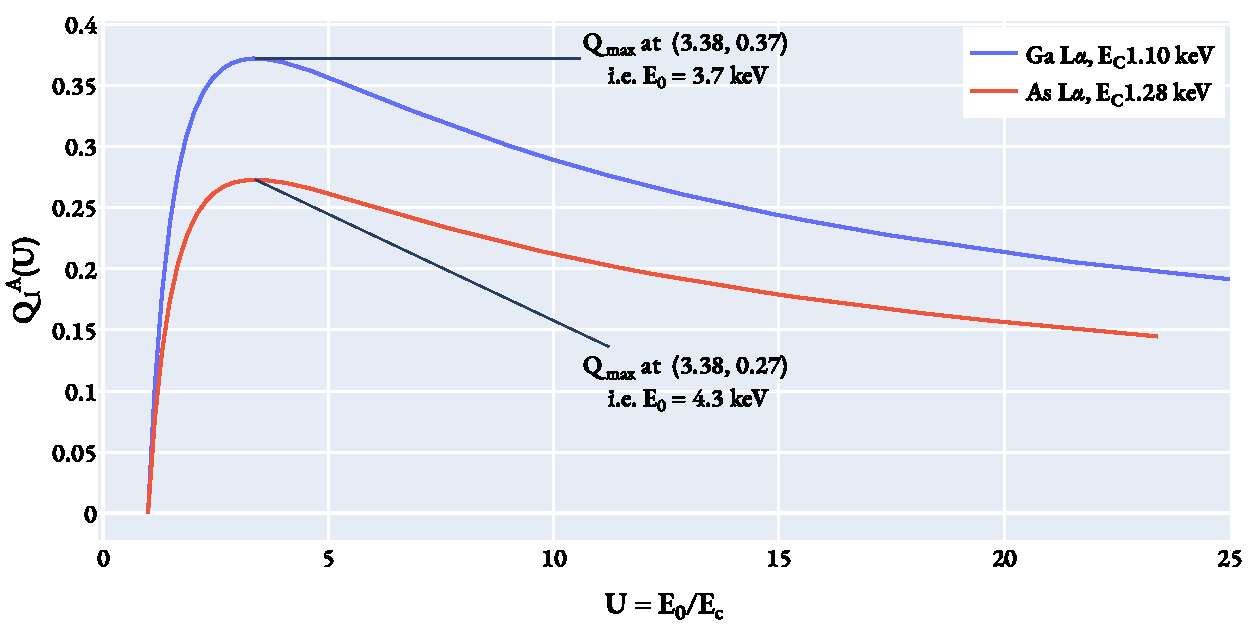
\includegraphics[width=0.8\textwidth]{figures/PAP_ionization_cross_section.pdf}
    \caption{
        Ionization cross section, $Q$ as a function of overvoltage Ga L$\alpha$ and As L$\alpha$.
        The maximum $Q$ is annotated, which is at the same overvoltage, but different energies due to different $E_C$.
    }
    \label{fig:PAP:ionization_cross_section}
\end{figure}



The average energy loss ($dE/d\rho s$) is not calculated from the law of Bethe, as that equation is not valid for low energies \cite{inokuti_on_bethe_1971,pap_1991}.
Instead, the PAP model calculate the average energy loss from the equation:

% dE/d rho s = - (M/J) * (1/f(V))

\begin{equation}
    \label{eq:theory:quantitative:pap:calculation_of_F:dE_d_rho_s}
    \frac{dE}{d\rho s} = - \frac{M}{J} \frac{1}{f(V)}
\end{equation}

Where:
\begin{equation}
    \label{eq:theory:quantitative:pap:calculation_of_F:dE_d_rho_s:M}
    M = \sum \limits_{i} \frac{C_i Z_i}{A_i}
\end{equation}

\begin{equation}
    \label{eq:theory:quantitative:pap:calculation_of_F:dE_d_rho_s:J}
    J = \exp(\sum \limits_{i} \frac{C_i Z_i}{A_i} \cdot \ln(J_i)/M)
\end{equation}

\begin{equation}
    \label{eq:theory:quantitative:pap:calculation_of_F:dE_d_rho_s:Ji}
    J_i = 10^{-3} \cdot Z_i (10.04 + 8.25 \exp(\frac{-Z_i}{11.22}))
\end{equation}

\begin{equation}
    \label{eq:theory:quantitative:pap:calculation_of_F:dE_d_rho_s:one_over_f}
    f(V) = \sum \limits_{k=1}^{3} D_k \cdot V^{P_k}
\end{equation}

$M$ is the mean ionization potential of the specimen, and $J$ is the mean ionization potential of the specimen, $J_i$ is the mean ionization potential of element $i$, and $f(V)$ is a function containing the energy dependent terms which makes \cref{eq:theory:quantitative:pap:calculation_of_F:dE_d_rho_s} equal to Bethe's law for high energies and still being valid for low energies. $V = E/J$, and $D_k$ and $P_k$ are constants, calculated as:


\begin{equation}
    \label{eq:theory:quantitative:pap:calculation_of_F:dE_d_rho_s:one_over_f:d_k}
    D_k = \begin{cases}
        D_1 = 6.6 \cdot 10^{-6}                                 \\
        D_2 = 1.12 \cdot 10^{-5}(1.35 - 0.45 J^2) \qquad \qquad \\
        D_3 = \frac{2.2 \cdot 10^{-6}}{J}
    \end{cases}
    P_k = \begin{cases}
        P_1 =  0.78 \\
        P_2 = 0.1   \\
        P_3 =  -(0.5-0.25J)
    \end{cases}
\end{equation}

% \begin{itemize}
%     \item $D_1 = 6.6 \cdot 10^{-6}$
%     \item $D_2 = 1.12 \cdot 10^{-5}(1.35 - 0.45 J^2)$
%     \item $D_3 = \frac{2.2 \cdot 10^{-6}}{J}$
%     \item $P_1 = 0.78$
%     \item $P_2 = 0.1$
%     \item $P_3 = -(0.5-0.25J)$
% \end{itemize}

i.e.

\begin{equation}
    \label{eq:theory:quantitative:pap:calculation_of_F:dE_d_rho_s:one_over_f_2}
    f(V) = 6.6 \cdot 10^{-6}\cdot V^{0.78} + 1.12\cdot 10^{-5}\cdot (1.35 - 0.45 J^2) \cdot V^{0.1} + \frac{2.2 \cdot 10^{-6}}{J} \cdot V^{-(0.5-0.25J)}
\end{equation}


\brynjar{Add a table with the constants and their units?}


The analytical solution for $1/S$ through the expression for the ionization cross section and the deceleration of the electrons, where $ T_K = 1 + P_k - m$:

\begin{equation}
    \label{eq:theory:quantitative:pap:calculation_of_F:dE_d_rho_s:analytical}
    1/S = \frac{U_0}{V_0 \cdot M} \sum \limits_{k=1}^{3} D_k \cdot (V_0/U_0)^{P_k} \cdot ((T_k)U_0^{T_k} \cdot \ln(U_0)-U_0^{T_k}+1)/T_k^2
\end{equation}


% Which translates to

% $1/S = \frac{U_O}{V_0 \cdot M} \cdot \\
% (6.6 \cdot 10^{-6} (V_0/U_0)^{0.78} \cdot ((1+0.78-m)U_0^{1+0.78-m} \cdot \ln(U_0)-U_0^{1+0.78-m}+1)/(1+0.78-m)^2) + \\
% ((1.12 \cdot 10^{-5}(1.35-0.45J^2)) (V_0/U_0)^{0.1} \cdot ((1+0.1-m)U_0^{1+0.1-m} \cdot \ln(U_0)-U_0^{1+0.1-m}+1)/(1+0.1-m)^2) + \\
% (2.2 \cdot 10^{-6}/J (V_0/U_0)^{(-0.5 +0.25J)} \cdot ((1+(-0.5 +0.25J)-m)U_0^{1+(-0.5 +0.25J)-m} \cdot \ln(U_0)-U_0^{1+(-0.5 +0.25J)-m}+1)/(1+(-0.5 +0.25J)-m)^2)
% $

The equation above is written out in the notebook for the PAP model.
\cref{fig:PAP:energy_loss_electrons_dE_drhos} show the energy loss of the electrons in GaAs, GaSb, and Cu, according to the PAP model.


% figures/PAP_energy_loss_dE_drhos.pdf
\begin{figure}[htbp]
    \centering
    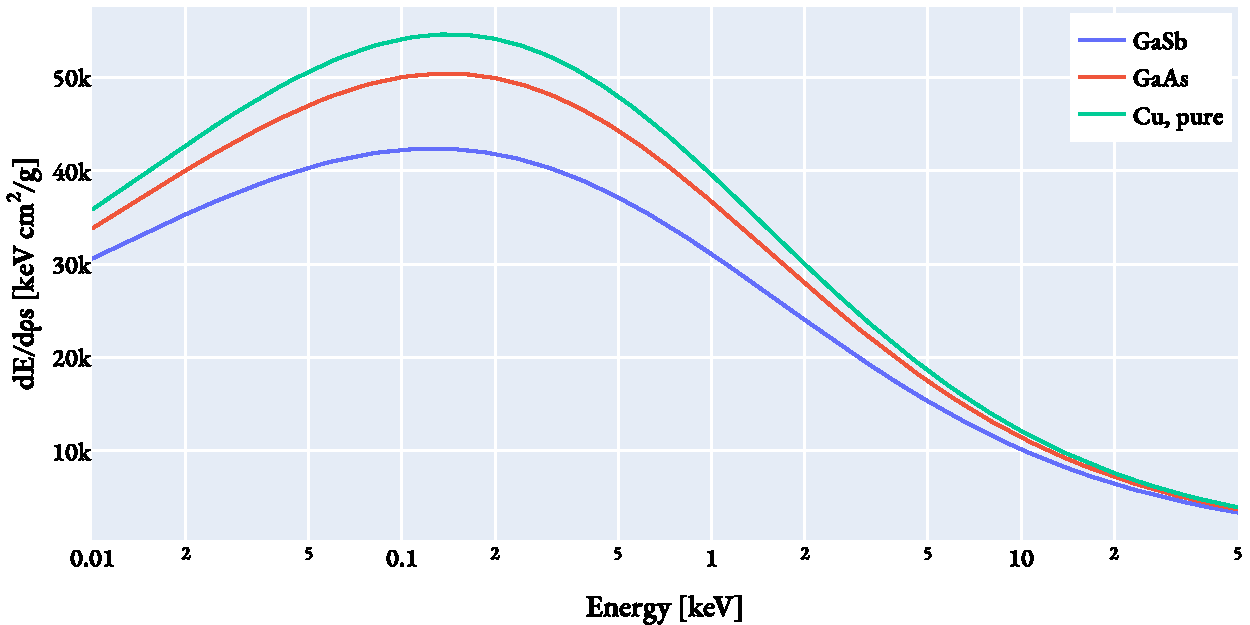
\includegraphics[width=0.8\linewidth]{figures/PAP_energy_loss_dE_drhos.pdf}
    \caption{
        The energy loss of electrons, $dE/d\rho s$,  in GaAs, GaSb, and Cu.
        Cu is added for reference to figure 4 in the PAP paper \cite{pap_1991}.
        The x-axis is logarithmic.
    }
    \label{fig:PAP:energy_loss_electrons_dE_drhos}
\end{figure}




% \subsubsection*{\emph{The backscattering factor,} $R$}

\paragraph*{\emph{The backscattering loss factor $R$}} is the fraction of the electrons that are backscattered from the specimen, calculated from the equation:
% The backscattering loss factor $R$ is calculated from the equation:

% $  $
\begin{equation}
    \label{eq:theory:quantitative:pap:calculation_of_F:R}
    R = 1- \bar{\eta}  \cdot \bar{W} \cdot (1-G(U_0))
\end{equation}

Where:

\begin{itemize}
    \item  $\bar{W} = \bar{E}_r/E_0 = 0.595 + \bar{\eta}/3.7 + \bar{\eta}^{4.55} $
    \item  $\bar{\eta} = 1.75 \cdot 10^{-3} \cdot \bar{Z}_b + 0.37(1-\exp(-0.015\bar{Z}_b^{1.3})) $
    \item  $\bar{Z}_b = (\sum C_i \cdot Z_i^{0.5})^2$
    \item  $G(U_0) = (U_0 - 1 - (1- \frac{1}{U_0^{1+q}})/(1+q)) / ((2+q)\cdot J(U_0))$
    \item  $J_G(U_0) = 1 + U_0 \cdot (\ln(U_0)-1) $
    \item  $q = (2 \bar{W} - 1) / (1 - \bar{W}) $
\end{itemize}


$\bar{\eta}$ is the mean backscattering coefficient\footnote{It looks like $\bar{\eta}$ is raised to (-4.55), but that is not the case. The difference between a bar and a minus is small, but crucial.}, $\bar{W}$ is the mean reduced energy of the backscattered electron, $\bar{Z}_b$ is the weighted mean atomic number, and $U_0$ is the overvoltage.
$G(U_0)$ is an equation from Coulon and Zeller \cite[Reference 28]{pap_1991}, calculated with $J_G(U_0)$ and $q$.
The backscattering factor for Z=1 to Z=90 is plottet with different overvoltages in \cref{fig:PAP:backscattering_factor}.

% figures/PAP_backscattering_factor.pdf

\begin{figure}[htbp]
    \centering
    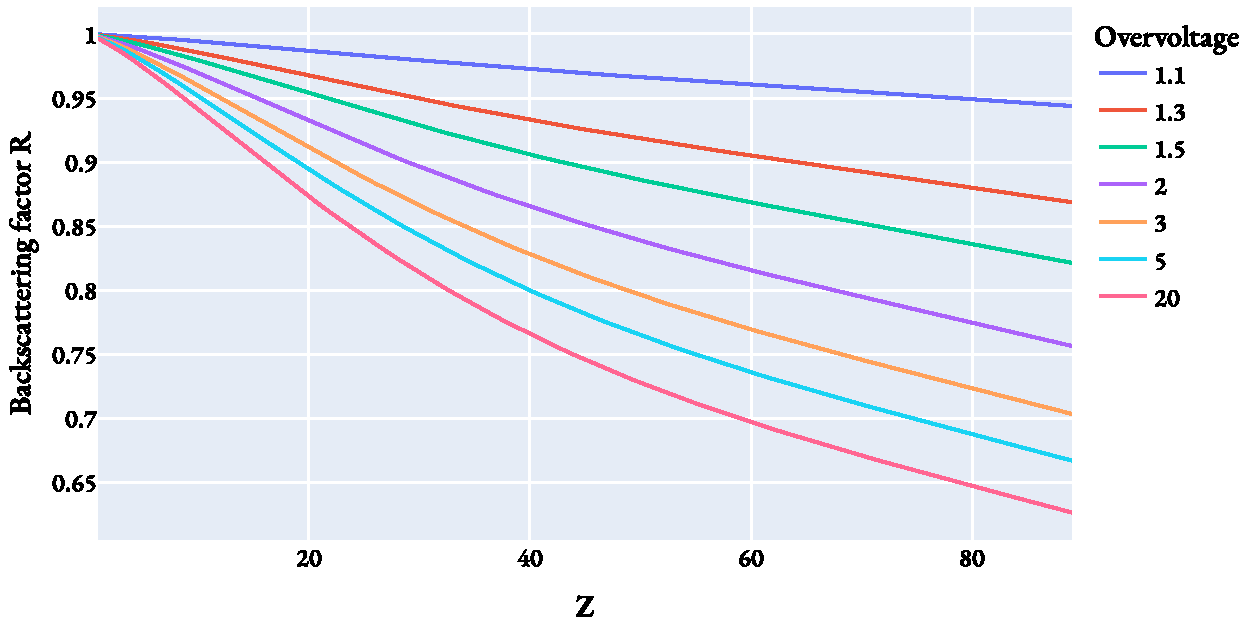
\includegraphics[width=0.8\linewidth]{figures/PAP_backscattering_factor.pdf}
    \caption{
        Backscattering factor for Z=1 to Z=90, with different overvoltages.
        The atomic number is on the x-axis, and the backscattering factor is on the y-axis.
        The different lines are for different overvoltages.
    }
    \label{fig:PAP:backscattering_factor}
\end{figure}





\subsubsection{PAP/XPP (b) Emergent intensity through parabolic representation of $\phi(\rho z)$}

The system of equations which lead to the parabolic representation of $\phi(\rho z)$ is given in the original paper \cite{pap_1991}, and is not repeated here.
The section covers the necessary calculations to find the emitted intensity, which is described as the "Simplified model: XPP".
The structure of the XPP model is similar to the PAP model, and XPP is chosen in this work as it is the model which is used in AZtec \brynjar{cite}.
Thus, the following equations are from the XPP model.


The emergent intensity of a specimen is given by \cref{eq:theory:quantitative:pap:general_principle:I_A} and the definition of $F(\chi)$ is given by \cref{eq:theory:quantitative:pap:general_principle:f_of_chi}. The analytical solution of $F(\chi)$ is given by:


% F(\chi) = \frac{A}{a+ \chi} + \frac{\phi(0) - A}{b + \chi} + \frac{B}{(b + \chi)^2}

\begin{equation}
    \label{eq:theory:quantitative:pap:F_of_chi}
    F(\chi) = \frac{A}{a+ \chi} + \frac{\phi(0) - A}{b + \chi} + \frac{B}{(b + \chi)^2}
\end{equation}

Where $A$, $B$, $a$ and $b$ are parameters of the parabolic representation of $\phi(\rho z)$, and $\phi(0)$ is the surface ionization\footnote{Appendix 4 about the XPP model also inculde $\varepsilon = (a-b)/b$ and a slightly different formulation of $F(\chi)$, but that is only a refactorization of \cref{eq:theory:quantitative:pap:F_of_chi}.}. The absorption correction factor can then be calculated by:

% f(chi) = F(chi)/F
\begin{equation}
    \label{eq:theory:quantitative:pap:absorption_correction}
    f(\chi) = \frac{F(\chi)}{F}
\end{equation}







% \subsubsection*{\emph{Surface ionization potential} $\phi(0)$ \emph{and the slope} $P$}
% \subsubsection*{\emph{Calculating} $\phi(0)$, $\bar{R}$, \emph{and} $P$}
\paragraph*{\emph{Calculating the surface ionization potential $\phi(0)$, the mean depth of ionization $\bar{R}$, and the initial slope $P$}} is the next step in the XPP model.
These three parameters are used to calculate $A$, $B$, $a$, and $b$, which is used to get the parabolic representation $F(\chi)$ for $\phi(\rho z)$.


The surface ionization potential is the amount of ionization happening at the surface of the specimen, which is the starting point for the $\phi(\rho z)$ curve. The surface ionization potential is given by:

% $\phi(0) = 1 + 3.3 (1-1/U_0^r)* \bar{\eta}^{1.2} $
\begin{equation}
    \label{eq:theory:quantitative:pap:phi_0}
    \phi(0) = 1 + 3.3 (1-1/U_0^{2 - 2.3 \bar{\eta}}) \cdot \bar{\eta}^{1.2}
\end{equation}


The surface ionization potential, $\phi(0)$ is illustrated for Z=1 to Z=90 with differing overvoltages in \cref{fig:pap:phi_0}.


% figures/PAP_surface_ionization_potential.pdf
\begin{figure}[htbp]
    \centering
    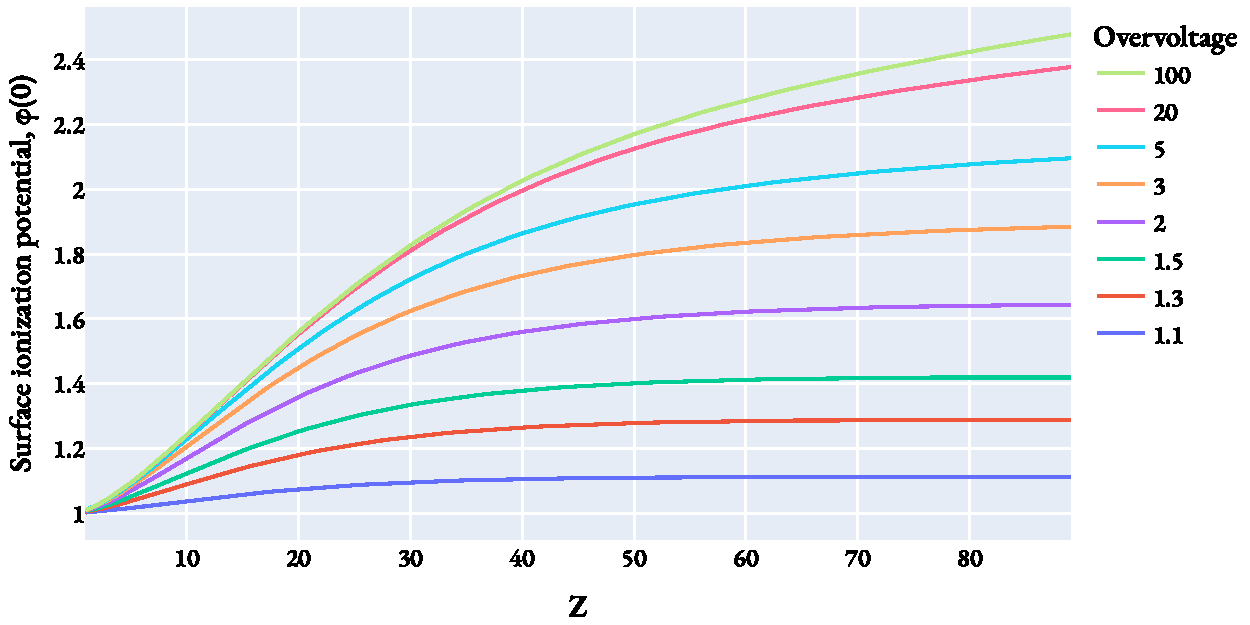
\includegraphics[width=0.8\linewidth]{figures/PAP_surface_ionization_potential.pdf}
    \caption{
        Surface ionization potential for Z=1 to Z=90, with different overvoltages.
        The atomic number is on the x-axis, and the surface ionization potential is on the y-axis.
        The different lines are for different overvoltages.
    }
    \label{fig:pap:phi_0}
\end{figure}

The average depth of ionization, $\bar{R}$, is given by:

% $ \bar{R} = F / (1 + [X \cdot \ln(1 + Y \cdot (1 - 1/U_0^{0.42}))]/\ln(1 + Y)) $
\begin{equation}
    \label{eq:theory:quantitative:pap:R_bar}
    \bar{R} = F / (1 + [X \cdot \ln(1 + Y \cdot (1 - 1/U_0^{0.42}))]/\ln(1 + Y))
\end{equation}

Where $X$ and $Y$ are given by:

\begin{itemize}
    \item $ X = 1 + 1.3 \ln(\bar{Z}_b) $
    \item $ Y = 0.2 + \bar{Z}_b/200 $
\end{itemize}



It is stated in the XPP computation scheme that "If $ F/\bar{R} < \phi(0) $, impose the condition $ \bar{R} = F/\phi(0) $" \cite[Appendix 4]{pap_1991}.
\brynjar{Implement this check.}


The initial slope $P$ is given by:

\begin{equation}
    \label{eq:theory:quantitative:pap:slope_P}
    P = g \cdot h^4 \cdot F/\bar{R}^2
\end{equation}

Where $g$ and $h$ are given by:

\begin{itemize}
    \item $ g = 0.22 \ln(4 \bar{Z}_b) \cdot [1 - 2 \exp(-\bar{Z}_b \frac{U_0 - 1}{15})] $
    \item $ h = 1 - 10(1-\frac{1}{1+ U_0/10})/\bar{Z}_b^2 $
\end{itemize}


The slope $P$ have a similar comment as $\bar{R}$, which states that "If necessary, limit the value $ g \cdot h^4 $ to the value $ 0.9 \cdot b\cdot  \bar{R}^2 \cdot [b - 2 \phi(0)/F] $".
\brynjar{Implement this too.}








% \subsubsection*{\emph{Calculating} $A$, $B$, $a$, \emph{and} $b$}


\paragraph{\emph{The parameters $A$, $B$, $a$, and $b$}} are used to calculate the parabolic representation $F(\chi)$ for $\phi(\rho z)$.
They can also be used to calculate $\phi(\rho z)$, which is done further down.
Additionally, the parameter $\varepsilon$ is used to easen the calculation of $A$ and $B$.
The parameters are calculated sequentially, starting with $b$, then $a$, then $\varepsilon$, then $B$, and finally $A$.


\begin{equation}
    \label{eq:theory:quantitative:pap:small_b}
    b = \sqrt{2} \cdot (1 + \sqrt{1 - \bar{R} \cdot \phi(0) / F})/\bar{R}
\end{equation}

\begin{equation}
    \label{eq:theory:quantitative:pap:small_a}
    a = [P + b \cdot (2\phi(0) - b \cdot F)] / [b \cdot F \cdot (2 - b \bar{R}) - \phi(0)]
\end{equation}

\begin{equation}
    \label{eq:theory:quantitative:pap:epsilon}
    \varepsilon = \frac{a-b}{b}
\end{equation}

The PAP paper have the following comment on the value of $\varepsilon$: "If necessary, impose on $\varepsilon$ a minimum absolute value (e.g. $10^{-6}$), and then assume $ a = b \cdot(1+\varepsilon) $".
If the author understands this correctly, the comment is aimed on computational issues in the 90s where values too close to zero would cause numerical issues.
Thus, this is not implemented in the code, as it is not necessary with modern computers.


The parameter $A$ and $B$ are then calculated by:

\begin{equation}
    \label{eq:theory:quantitative:pap:big_B}
    B = [b^2 \cdot F \cdot (1 + \varepsilon) - P - \phi(0) \cdot b \cdot (2+\varepsilon) ] / \varepsilon
\end{equation}

\begin{equation}
    \label{eq:theory:quantitative:pap:_big_A}
    A = [B/b + \phi(0) - b \cdot F] \cdot \frac{1+ \varepsilon}{\varepsilon}
\end{equation}


With $A$, $B$, $a$, $b$ and $\phi(0)$ calculated, the absorption correction $f(\chi$) and the emergent intensity through $F(\chi$) can be calculated with \cref{eq:theory:quantitative:pap:absorption_correction} and \cref{eq:theory:quantitative:pap:F_of_chi} respectively.


That covers the necessary theory for the XPP model to be implemented in code.


\paragraph{Plotting the depth distribution $\phi(\rho z)$} can be done with the now calculated parameters $A$, $B$, $a$, $b$ and $\phi(0)$.
It is useful to plot $\phi(\rho z)$ and the other functions in the XPP model to see how the model behaves, and to see if the model is implemented correctly by comparing the plots to the plots in the PAP paper.
It is the absorption correction factor given in \cref{eq:theory:quantitative:pap:absorption_correction} that is used and tested on the EDS data acquired in this work.
\cref{fig:pap:phi_of_rhoz} is a plot of $\phi(\rho z)$ for Ga L$\alpha$ in GaAs.
The curve is calculated with the following equation for $\phi(\rho z)$ is given in the PAP paper:

% $  $

\begin{equation}
    \label{eq:theory:quantitative:pap:phi_of_rho_z}
    \phi (\rho z) = A \cdot \exp(- a \cdot (\rho z)) + (B \cdot (\rho z) + \phi(0) - A) \cdot \exp(- b \cdot (\rho z))
\end{equation}


% figures/PAP_phi_of_rhoz.pdf
\begin{figure}[htbp]
    \centering
    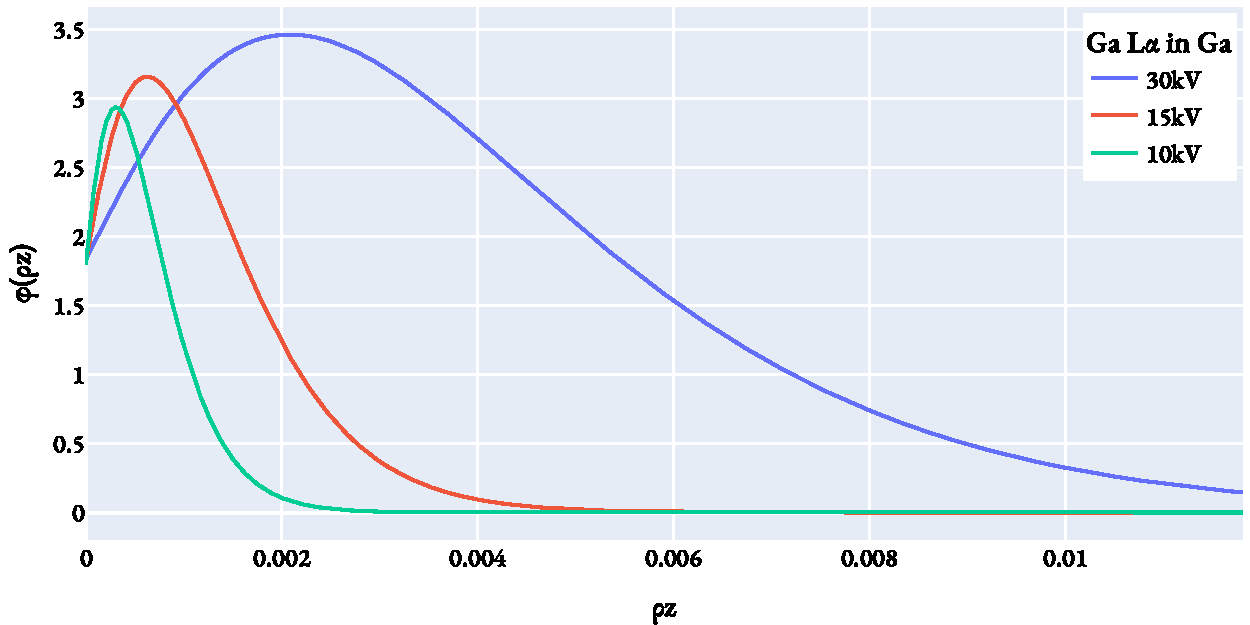
\includegraphics[width=0.8\linewidth]{figures/PAP_phi_of_rhoz.pdf}
    \caption{
        Plot of $\phi(\rho z)$ for Ga L$\alpha$ in GaAs.
        The plot show three different beam energies, 15 (blue), red (10), and 5 (green) keV.
        \brynjar{As of now, the numbers on the y-axis are correct, but the x-axis is off by a factor of 10, I think.}
    }
    \label{fig:pap:phi_of_rhoz}
\end{figure}






\subsubsection{Additional comment to the PAP/XPP procedure}

Section II.E in the PAP paper is discussing the absorption coefficients for the PAP model, and Appendix 5 lists some values for $\mu_\rho$ associated with the PAP procedure \cite{pap_1991}.
These numbers are in the same range as the numbers provided by HyperSpy, but there are deviations.
For example, the line As L$\alpha$ in GaAs bulk is given $\mu_\rho = 7000$ in the PAP paper, and the value $\mu_\rho = 3744$ by Hyperspy.
Cu L$\alpha$ in pure Cu is given $\mu_\rho = 1755$ in the PAP paper, and $\mu_\rho = 1515$ by HyperSpy.
Cu L$\beta$ in pure Cu is given $\mu_\rho = 750$ in the PAP paper, while HyperSpy give $\mu_\rho = 8763$ for Cu L$\beta1$.
These deviations might be a source of error, which would lead to some adjustments of the PAP or XPP equations.
Such corrections might have been published as an update to the PAP/XPP procedure in a more recent paper, and can have been implemented by Oxford Instruments in their AZtec software to allow for more accurate quantification with updated constants and equations.
Investigating such possibilities are outside scope of this work, and might be a starting point for future work.




